\documentclass{article}
\usepackage{blindtext}
\usepackage{titlesec}
\usepackage{listings}
\usepackage{geometry}
\usepackage{mathtools}
\usepackage[utf8]{inputenc}
\usepackage{siunitx}
\usepackage{soul}
\usepackage{enumitem}
\usepackage{graphicx}
\usepackage{float}
\usepackage{units}
\usepackage{amsfonts}
\usepackage{graphicx}
\usepackage{amsfonts,amssymb,amsmath,hyperref}
\usepackage{color}
\usepackage{tcolorbox}
\usepackage[bottom]{footmisc}
\usepackage{tikz}
\usetikzlibrary{decorations.pathreplacing,shapes}
\usetikzlibrary{matrix}
\def\leftbracket{[}
\def\rightbracket{]}
\usetikzlibrary{calc}
\usepackage{physics}
\usepackage{minted}

\geometry{
 a4paper,
 total={170mm,257mm},
 left=20mm,
 top=20mm,
 }

\setlength{\parindent}{0pt}

\usetikzlibrary{matrix}
\def\leftbracket{[}
\def\rightbracket{]}

\tikzset{my dashed curvy arrow/.style={
  blue!60!black,
  ->,
  dashed,
  out=-90, in=90
  }
} 

\tikzset{my curvy arrow/.style={
  blue!60!black,
  ->,
  out=-90, in=90
  }
}

\tikzset{my arrow/.style={
  blue!60!black,
  -latex
  }
}

\tikzset{my green arrow/.style={
  green!60!black,
  -latex
  }
}

\tikzset{my red arrow/.style={
  red!60!black,
  -latex
  }
}

\begin{document}
\begin{titlepage}
	\centering
	{\scshape\LARGE Imperial College London \par}
	\vspace{2cm}
	{\scshape\Large Real-Time Digital Signal Processing \par}
	\vspace{1cm}
	{\scshape\Large Laboratory 4\par}
	\vspace{2.5cm}
	{\Large\itshape Ahmad Moniri, CID: 00842685 \par}
	\vspace{1cm}
	{\Large\itshape Pranav Malhotra, CID: 00823617 \par}
	\vfill
% Bottom of the page
	\begin{tcolorbox}
    \centering
    Declaration: We confirm that this submission is our own work. In it, we give references and citations whenever we refer to or use the published, or
    unpublished, work of others. We are aware that this course is bound by
    penalties as set out in the College examination offences policy \\~\\
    \underline{Signed: Ahmad Moniri, Pranav Malhotra}
    \end{tcolorbox}
	{\large \today\par}
\end{titlepage}

\newpage
\tableofcontents

\newpage
\section{Introduction}
In laboratory 3, interrupt-driven programming was introduced. Interrupt-driven programsare more efficient than programs that poll peripherals as they have the capacity to fully utilise the computation power of the processor/embedded device. As such, all programs written for the Real-Time Digital Signal Processing course from this point on will be interrupt-driven.\\ 

In laboratory 4, Finite Impulse Response (FIR) filters are introduced. Filter implementation is discussed and efficiency of different programming techniques is considered.\\

This report starts by introducing the theory behind FIR filters. Following this, design of FIR filters using MATLAB is discussed. Following this an in-depth analysis of the laboratory experiment is presented. The discussion includes multiple functions written in C to implement the convolution sum required for filtering. Next, before the different implementations are compared, the compiler present in the code composer environment is studied. The compiler offers in-built optimisation options and thus understanding this is critical for efficient filtering. The filter's spectrum is also validated using the Audio Precision $APX520$ device.

\section{Finite Impulse Response (FIR) Filters}\label{sec:FIR_theory}
A FIR filter, as the name finite suggests has an impulse response that reaches zero in a finite duration of time. This has an important implication; the memory in the system is finite. FIR filters can only be implemented digitally as analogue filters have an Infinite Impulse Response (IIR).\\ 

Equation (\ref{eq:fir_diff_eq}) shows the general form of the difference equation that represents a FIR filter. The number $M$ represents the order of the filter. \textbf{The order of the filter represents the amount of memory the system has.}\\

The difference equation can also be written as an inner product as shown in equation (\ref{eq:fir_conv_sum}).\textbf{ For a FIR filter, the filter coefficients are equivalent to impulse response of the filter\footnote{This does not apply for an IIR filter, since the impulse response is infinite.}.}

\begin{align}
    y[n]    &= b_{0}x[n] + b_{1}x[n-1] +  b_{2}x[n-2] + \cdots + b_{M}x[n-M]\label{eq:fir_diff_eq}\\ 
            &= \sum_{i=0}^{M}h[n]x[n-i]\label{eq:fir_conv_sum}
\end{align}

Taking the z-transform of equation (\ref{eq:fir_diff_eq}) returns the general form of the transfer function of a FIR filter presented in equation (\ref{eq:fir_transfer_func}). Equation (\ref{eq:fir_transfer_func_2}) corroborates the fact that the order of the filter is $M$\footnote{The order of the polynomial in the denominator of the transfer function determines the order of the filter.}. 


\begin{align}
    H(z) = \frac{Y(z)}{X(z)}    &= h[0] + h[1]z^{-1} + \cdots + h[M]z^{-M}\label{eq:fir_transfer_func}\\ 
                                &= \frac{h[0]z^{M} + h[1]z^{M-1} + \cdots + h[M]}{z^M} \label{eq:fir_transfer_func_2}
\end{align}

A zero in the transfer function causes a dip in the magnitude response of a filter and thus is not considered when stability of the filter is studied. The amount of attenuation is dependent on the distance of the zero, on the z-plane, from the unit circle. A zero placed close to the unit circle will cause greater attenuation than a zero that is placed further away from the unit circle. It is important to note that in the Real-Time Digital Signal Processing course, only real signals are considered and thus all coefficients are real. As a result, all zeroes are either real or occur in complex conjugate pairs. \textbf{The frequency response of a FIR filter with real coefficients will be symmetric about the half the sampling frequency\footnote{Symmetric about half the sampling frequency also means that the frequency response of symmetric about the y-axis in the frequency domain. Half of the sampling frequency is mentioned because the MATLAB function {\tt freqz} plots the frequency response of the filter from $0$ to $F_{s}$.}.} \\

In addition, it is clear that the FIR filter has $M$ poles located at the origin of the z-plane. Poles located outside the unit circle in the z-plane will result in an impulse response that grows exponentially. The system will not be Bounded-Input Bounded Output (BIBO) stable. \textbf{FIR filters are inherently stable as poles are always located at the origin.} Not having the freedom to place poles on the z-plane presents many limitations when a FIR filter is designed. To compensate, FIR filters have a significantly larger order than IIR filters that attain similar frequency responses. \textbf{Although FIR filters present stark limitations, in that poles are always located at the origin, they can be designed to have a linear phase response in the frequencies of interest.}\\

Equation (\ref{eq:fir_transfer_funct_3}) shows the general form of the transfer function of a FIR filter written as a convolution sum, where $h[n]$ represents the impulse response of the filter.

\begin{equation}\label{eq:fir_transfer_funct_3}
    H(z) = \frac{Y(z)}{X(z)} = \sum_{n=0}^{M}h[n]z^{-n}
\end{equation}

Equation (\ref{eq:fir_transfer_funct_3}) can be implemented using the signal flow graph shown in figure \ref{fig:direct_form_fir}.

\begin{figure}[H]
    \centering
    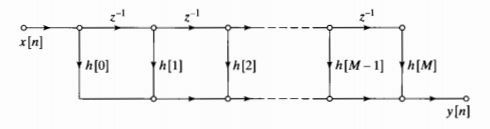
\includegraphics[width=0.8\textwidth]{filter1}
    \caption{Direct form of FIR filter}
    \label{fig:direct_form_fir}
\end{figure}

Next, consider a filter with an impulse response that is symmetric. The symmetric relation between the coefficients of the filter is explicitly stated in equation (\ref{eq:symmetric}), where $M$ is the order of the filter.

\begin{equation}\label{eq:symmetric}
    h[n] = h[M-1-n]
\end{equation}

The symmetric nature of the impulse allows for the following manipulations\footnote{It is assumed that the filter has an odd number of coefficients. Similar calculations can be performed for a filter with an even number of coefficients. These calculations are not presented in this report.},

\begin{align}
    H(z)    &= \sum_{n=0}^{M}h[n]z^{-n}\label{eq:fir_symmetric_tf}\\
            &= \sum_{n=0}^{\nicefrac{(M-3)}{2}}h[n]\Bigg(z^{-n}+z^{-(M-1-n)}\Bigg) + h(\tfrac{M-1}{2})z^{-\nicefrac{(M-1)}{2}} \label{eq:fir_symmetric_final}
\end{align}

Evaluating equation (\ref{eq:fir_symmetric_final}) for $z = e^{j\omega}$ will return the frequency response of the filter.

\begin{align}
    H(e^{j\omega})  &= \sum_{n=0}^{\nicefrac{(M-3)}{2}}h[n]\Bigg(e^{-j\omega n}+e^{-j\omega (M-1-n)}\Bigg) +                      h(\tfrac{M-1}{2})e^{-\nicefrac{j\omega (M-1)}{2}} \\
                    &= \sum_{n=0}^{\nicefrac{(M-3)}{2}}h[n]\Bigg(e^{+j\omega (n-\nicefrac{(M-1)}{2})}+e^{-j\omega (n-\nicefrac{(M-1)}{2})}\Bigg)e^{-\nicefrac{j\omega (M-1)}{2}} + h(\tfrac{M-1}{2})e^{-\nicefrac{j\omega (M-1)}{2}} \\
                    &= \sum_{n=0}^{\nicefrac{(M-3)}{2}}\Bigg(2h[n]cos(\omega(n-\tfrac{M-1}{2}))\Bigg)e^{\nicefrac{-j\omega (M-1)}{2}} + h(\tfrac{M-1}{2})e^{-\nicefrac{j\omega (M-1)}{2}}\\\label{eq:lin_phase}
                    &= \Bigg(e^{-\nicefrac{j\omega (M-1)}{2}}\Bigg)\Bigg(\sum_{n=0}^{\nicefrac{(M-3)}{2}}2h[n]cos(\omega(n-\tfrac{M-1}{2})) + h(\tfrac{M-1}{2})\Bigg) 
\end{align}

Based on equation (\ref{eq:lin_phase}), the magnitude response, phase response and group delay can be evaluated.
\begin{align}
       \quad& \Big|H(e^{j\omega})\Big| = \sum_{n=0}^{\nicefrac{(M-3)}{2}}2h[n]cos(\omega(n-\tfrac{M-1}{2})) + h(\tfrac{M-1}{2})\\
                    & \angle H(e^{j\omega}) = -\omega\frac{M-1}{2} \label{eq:phase} \\
                    & Group\:Delay = -\dv{\phi}{\omega} = \frac{M-1}{2} samples \label{eq:group_delay}
\end{align}\\

Equation (\ref{eq:phase}) shows that the phase response varies linearly with $\omega$. Such a phase response cannot be achieved with an IIR filter. Having a linear phase response is critical is many applications such as audio signal processing. The human ear is more sensitive to changes in phase than changes in magnitude. \textbf{A linear phase response means that the relative phase of the spectral components in the signal will be constant. The signal will however be delayed as it passes through the filter.} The delay, in terms of samples, is expressed in equation (\ref{eq:group_delay}). The delay in the time domain is calculated using, $\nicefrac{(M-1)t_{s}}{2}$ where $t_{s}$ is the sampling period. \\

Equation (\ref{eq:fir_symmetric_final}) can be implemented using the signal flow graph shown in figure \ref{fig:fir_symmetric_signal_flow}. \textbf{It is clear that the the symmetric nature of the impulse response can be exploited to half the number of multiplications required for filtering.} This will be discussed in greater detail in section \ref{sec:exploit_symmetry}.

\begin{figure}[H]
    \centering
    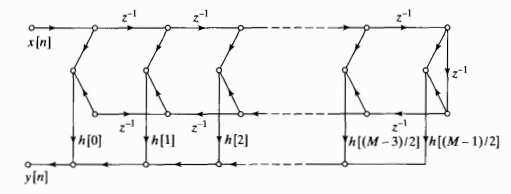
\includegraphics[width=0.8\textwidth]{filter2}
    \caption{Canonical form of FIR filter}
    \label{fig:fir_symmetric_signal_flow}
\end{figure}

\newpage
\section{Design of Filter using MATLAB}\label{sec:mat_design}
In laboratory 4, the filter described in figure \ref{fig:ideal_filter} has to be implemented.

\begin{figure}[H]
    \centering
    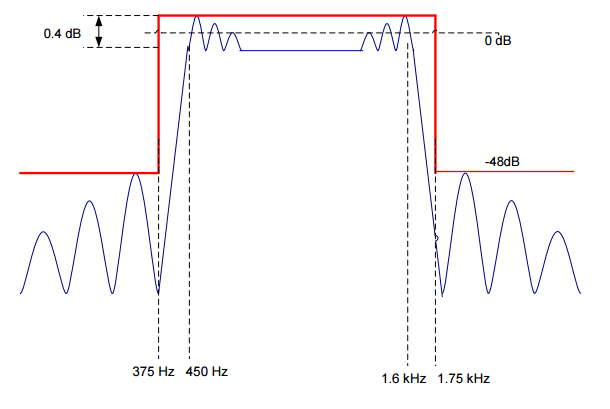
\includegraphics[width=0.6\textwidth]{ideal_filter}
    \caption{Filter to be implemented in laboratory 4}
    \label{fig:ideal_filter}
\end{figure}

The filter is designed in MATLAB and the code presented in listing \ref{lst:matlab_initial_filter}. The functions {\tt firpmord} and {\tt firpm} are used to design the filter. \textbf{The filter is designed using the Parks-McClellan algorithm and has an optimal frequency response. Optimality is defined as a filter that uses the least number of coefficients to just meet the specifications.} Having an equiripple design minimises the maximum error between the designed filter and the specifications at any particular frequency. Other designs algorithms are optimised to minimise other parameters. For example, the least squares design algorithm aims to minimise the total mean squared error.\\ 

\begin{listing}
\begin{minted}[fontsize=\scriptsize,linenos]{MATLAB}
rp = 0.4;                           % defines the pass band ripple
rs = 48;                            % defines the stop band attenuation
F_sampling = 8000;                  % defines the sampling frequency
F_cutoff = [375 450 1600 1750];     % defines the cutoff frequencies
filter_amplitudes = [0 1 0];        % defines ideal gain of each band

% function used to estimate variables need for firpm function
[N, Fo, Ao, W] = firpmord(  F_cutoff,...
                            filter_amplitudes,...
                            [10^(-rs/20) (10^(rp/20)-1)/(10^(rp/20)+1) 10^(-rs/20)],...
                            F_sampling);

                        
[coefs, error] = firpm(N+4, Fo, Ao, W);      % order of filter is increased by 4 to meet specifications

[h,w] = freqz(coefs, [1], 2^16);
\end{minted}
\caption{MATLAB code to generate coefficients for a FIR filter} 
\label{lst:matlab_initial_filter}
\end{listing}

\textbf{The function {\tt firpmord} requires the pass band deviation and stop band attenuation to be expressed in absolute terms as opposed to, in decibels}. Notice that the filter is specified in figure \ref{fig:ideal_filter} is specified in decibels and thus a conversion is necessary. The appropriate value for pass band deviation is calculated using the formula stated in equation (\ref{eq:passband_deviation}) where $rp$ represents the pass band ripple.

\begin{equation}\label{eq:passband_deviation}
    Passband \ Deviation = \frac{10^{\nicefrac{rp}{20}}-1}{10^{\nicefrac{rp}{20}}+1}
\end{equation}

\textbf{It should be noted that the function {\tt firpmord} only generates an estimate for the order of the filter. To meet all specifications of the filter, the estimated filter order was increased by 4.} Figure \ref{fig:matlab_filter} shows the magnitude and phase response of the filter that was generated. 

\begin{figure}[H]
    \centering
    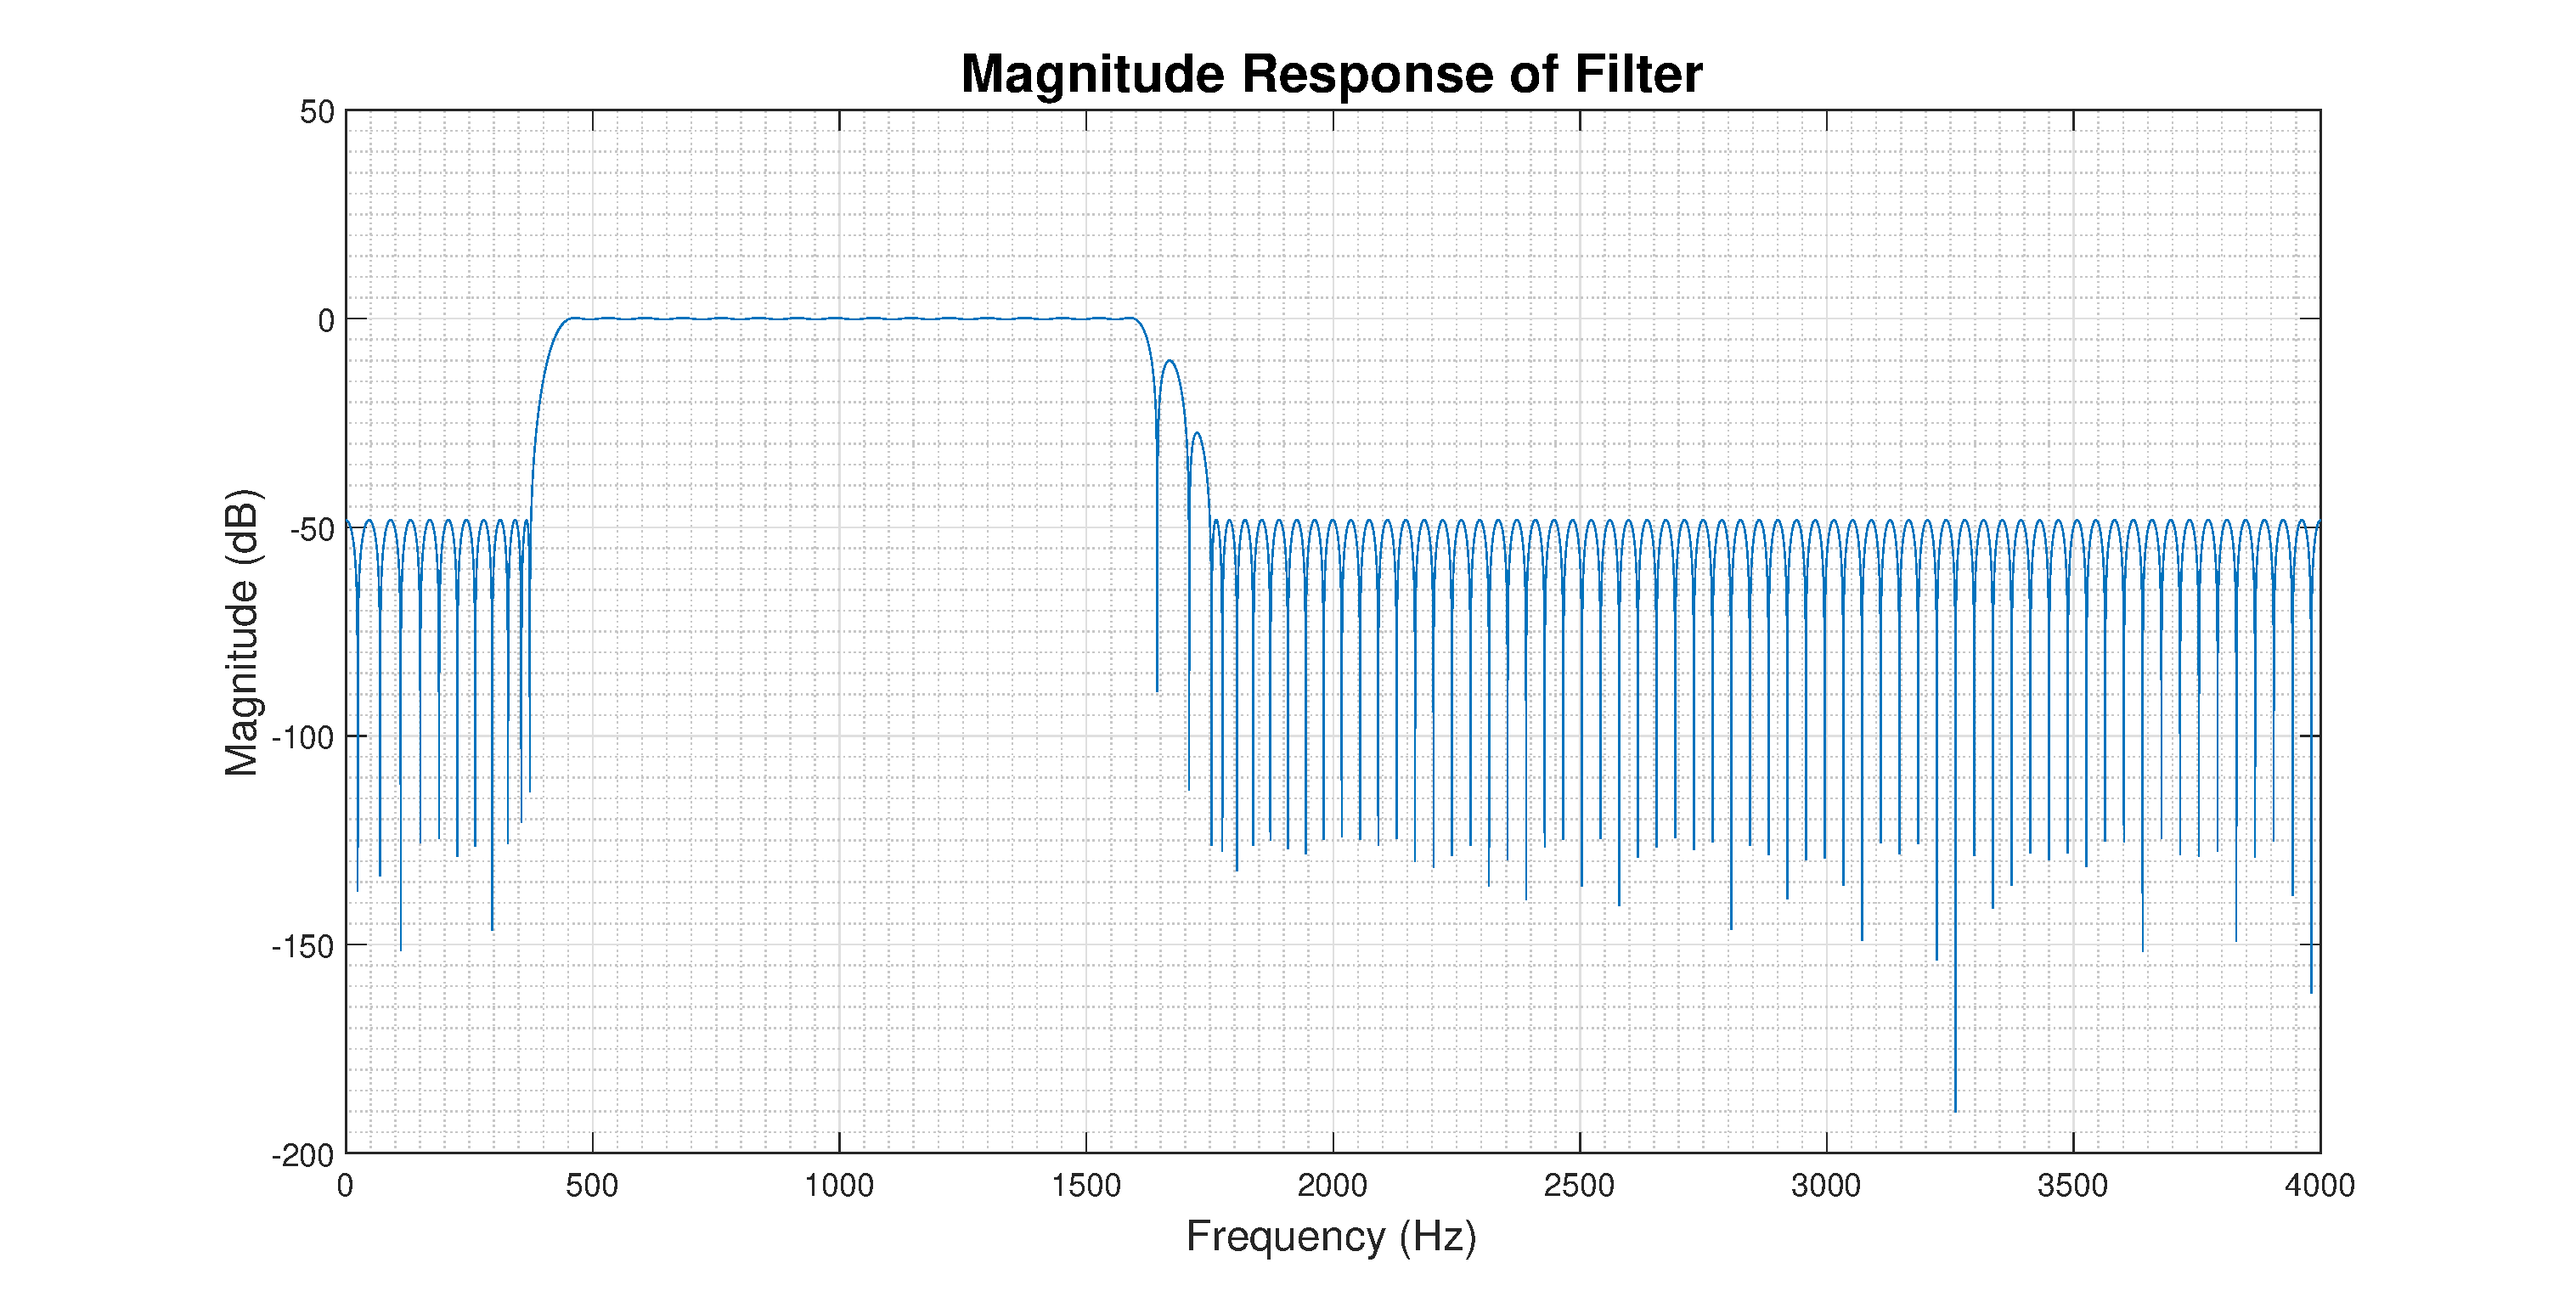
\includegraphics[width=0.49\textwidth]{mag_response_filter_1}
    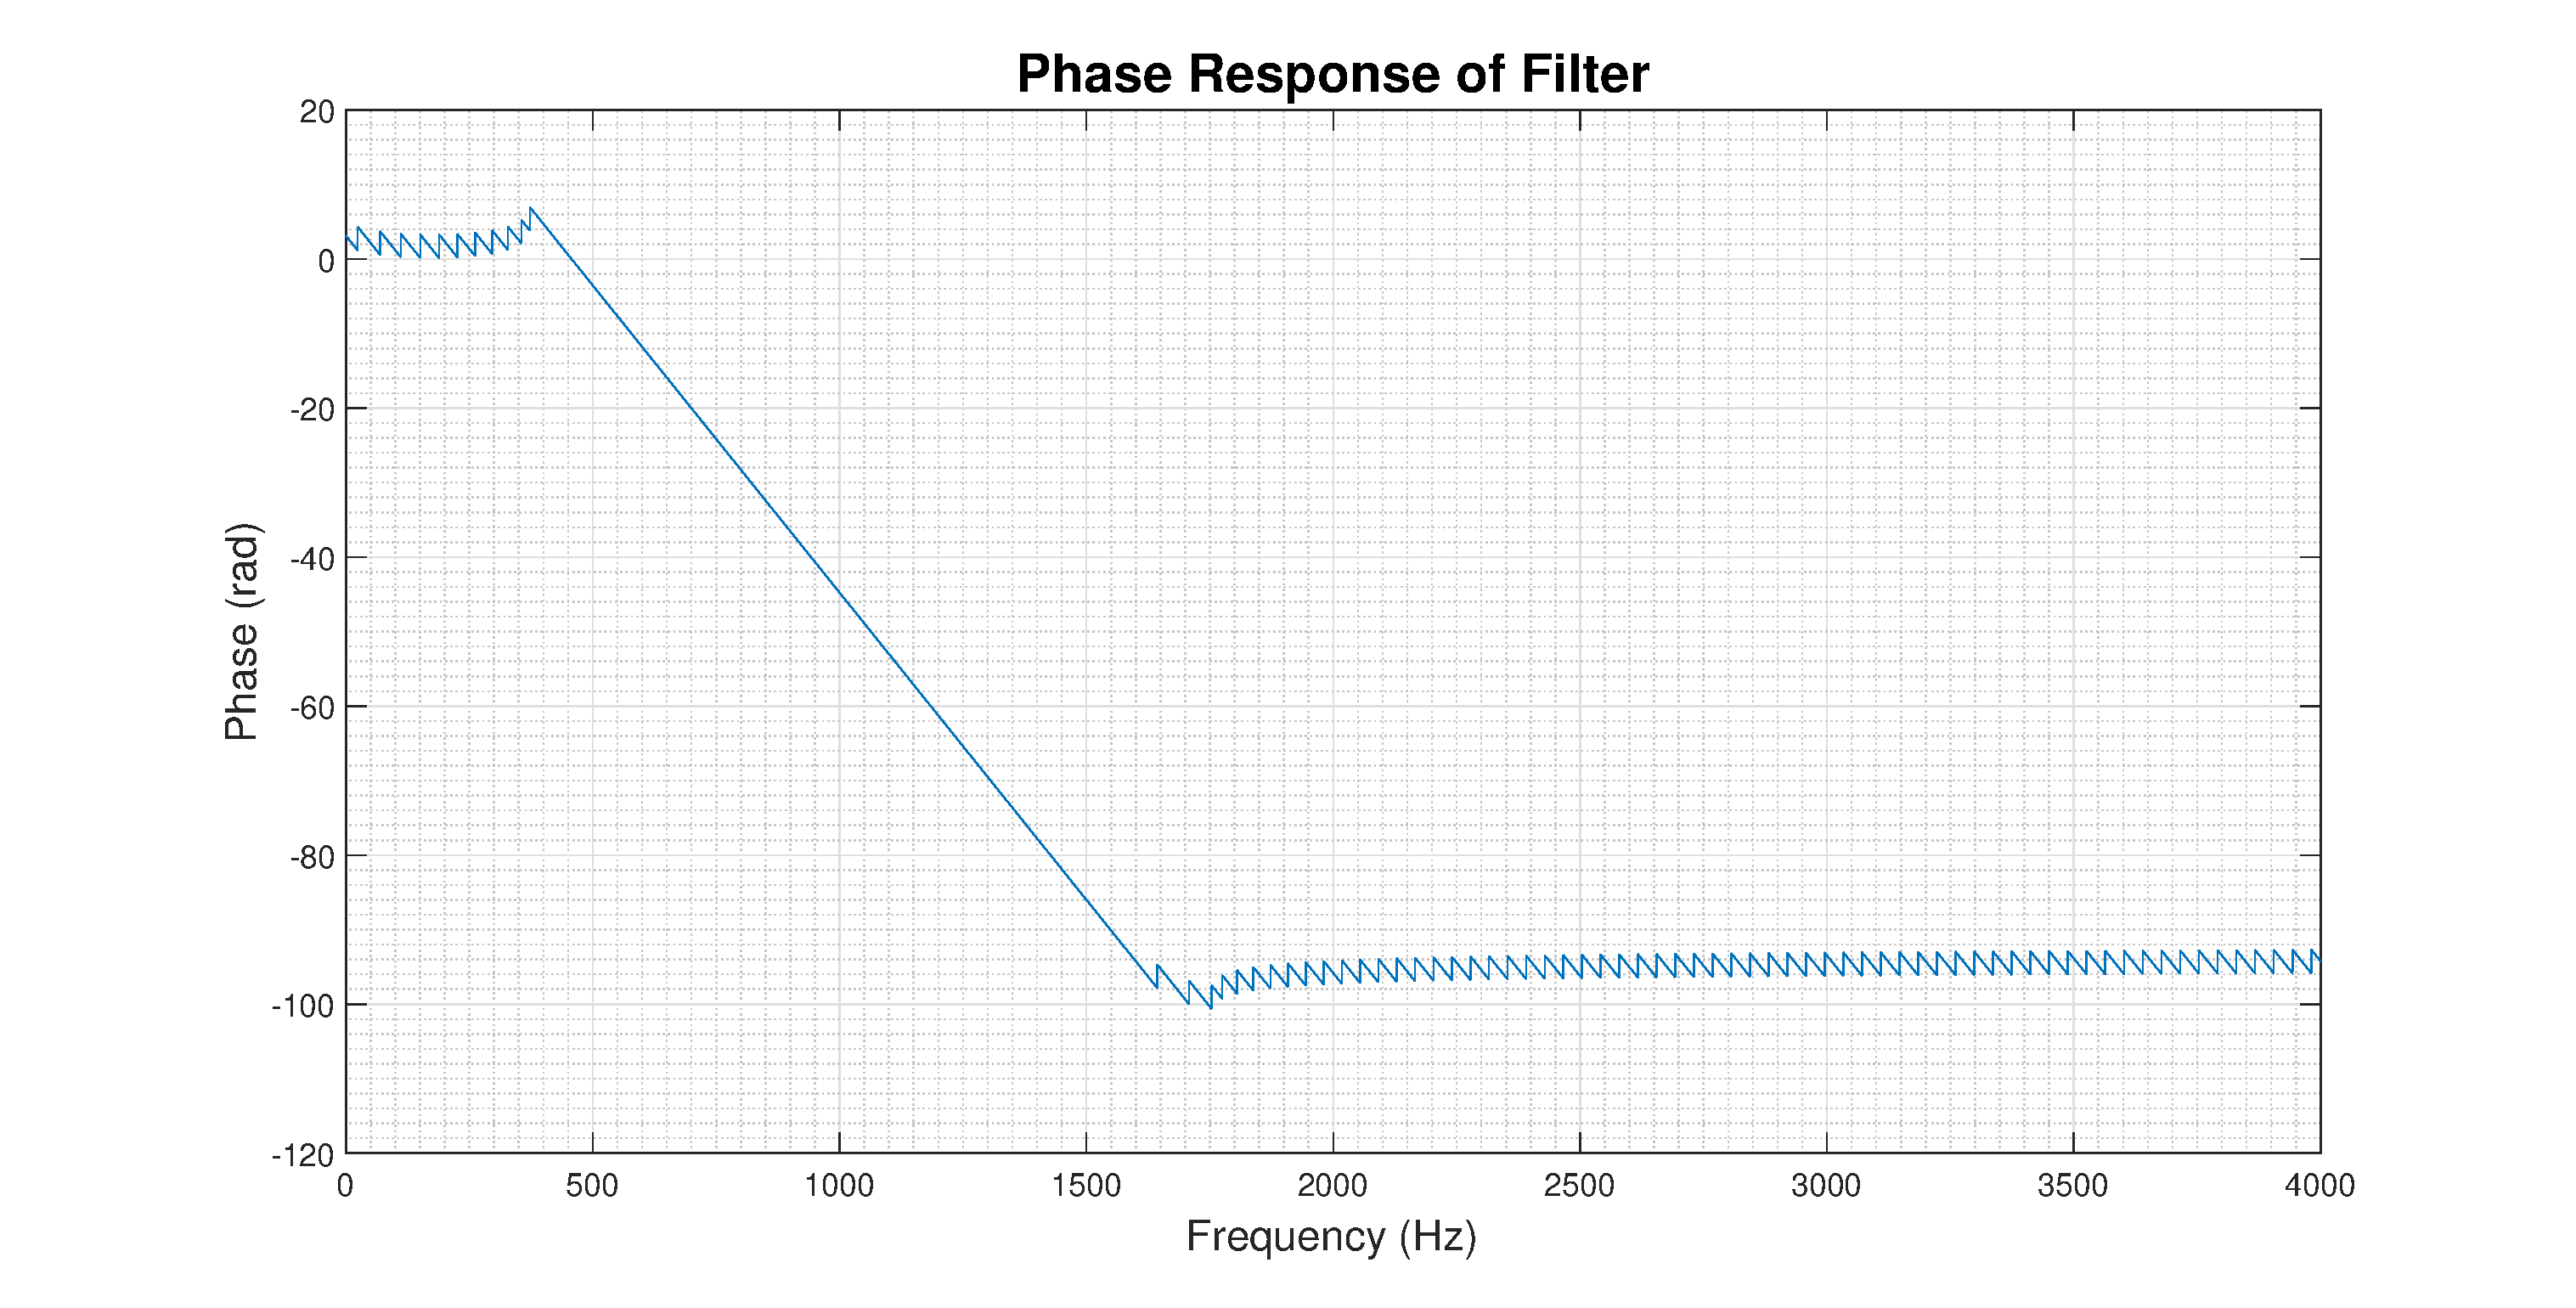
\includegraphics[width=0.49\textwidth]{phase_response_filter_1}
    \caption{Frequency response of designed filter}
    \label{fig:matlab_filter}
\end{figure}

\textbf{It is clear that the filter has a linear phase response in the pass band.} There is a non-linear phase response in the transition band and because zeros are extremely close to each other. Also, the zeros are not equidistant from the unit circle in the stopband. This is clear from the figure \ref{fig:filter_coefs}. \textbf{In the transition band, the dominant zeroes are placed equidistant from the unit circle to ensure a linear phase response. As discussed in section \ref{sec:FIR_theory}, an FIR filter has a linear phase response if the impulse response has the form described in equation (\ref{eq:symmetric}).} To verify this, the impulse response of the filter is graphed in figure \ref{fig:filter_coefs}.

\begin{figure}[H]
    \centering
    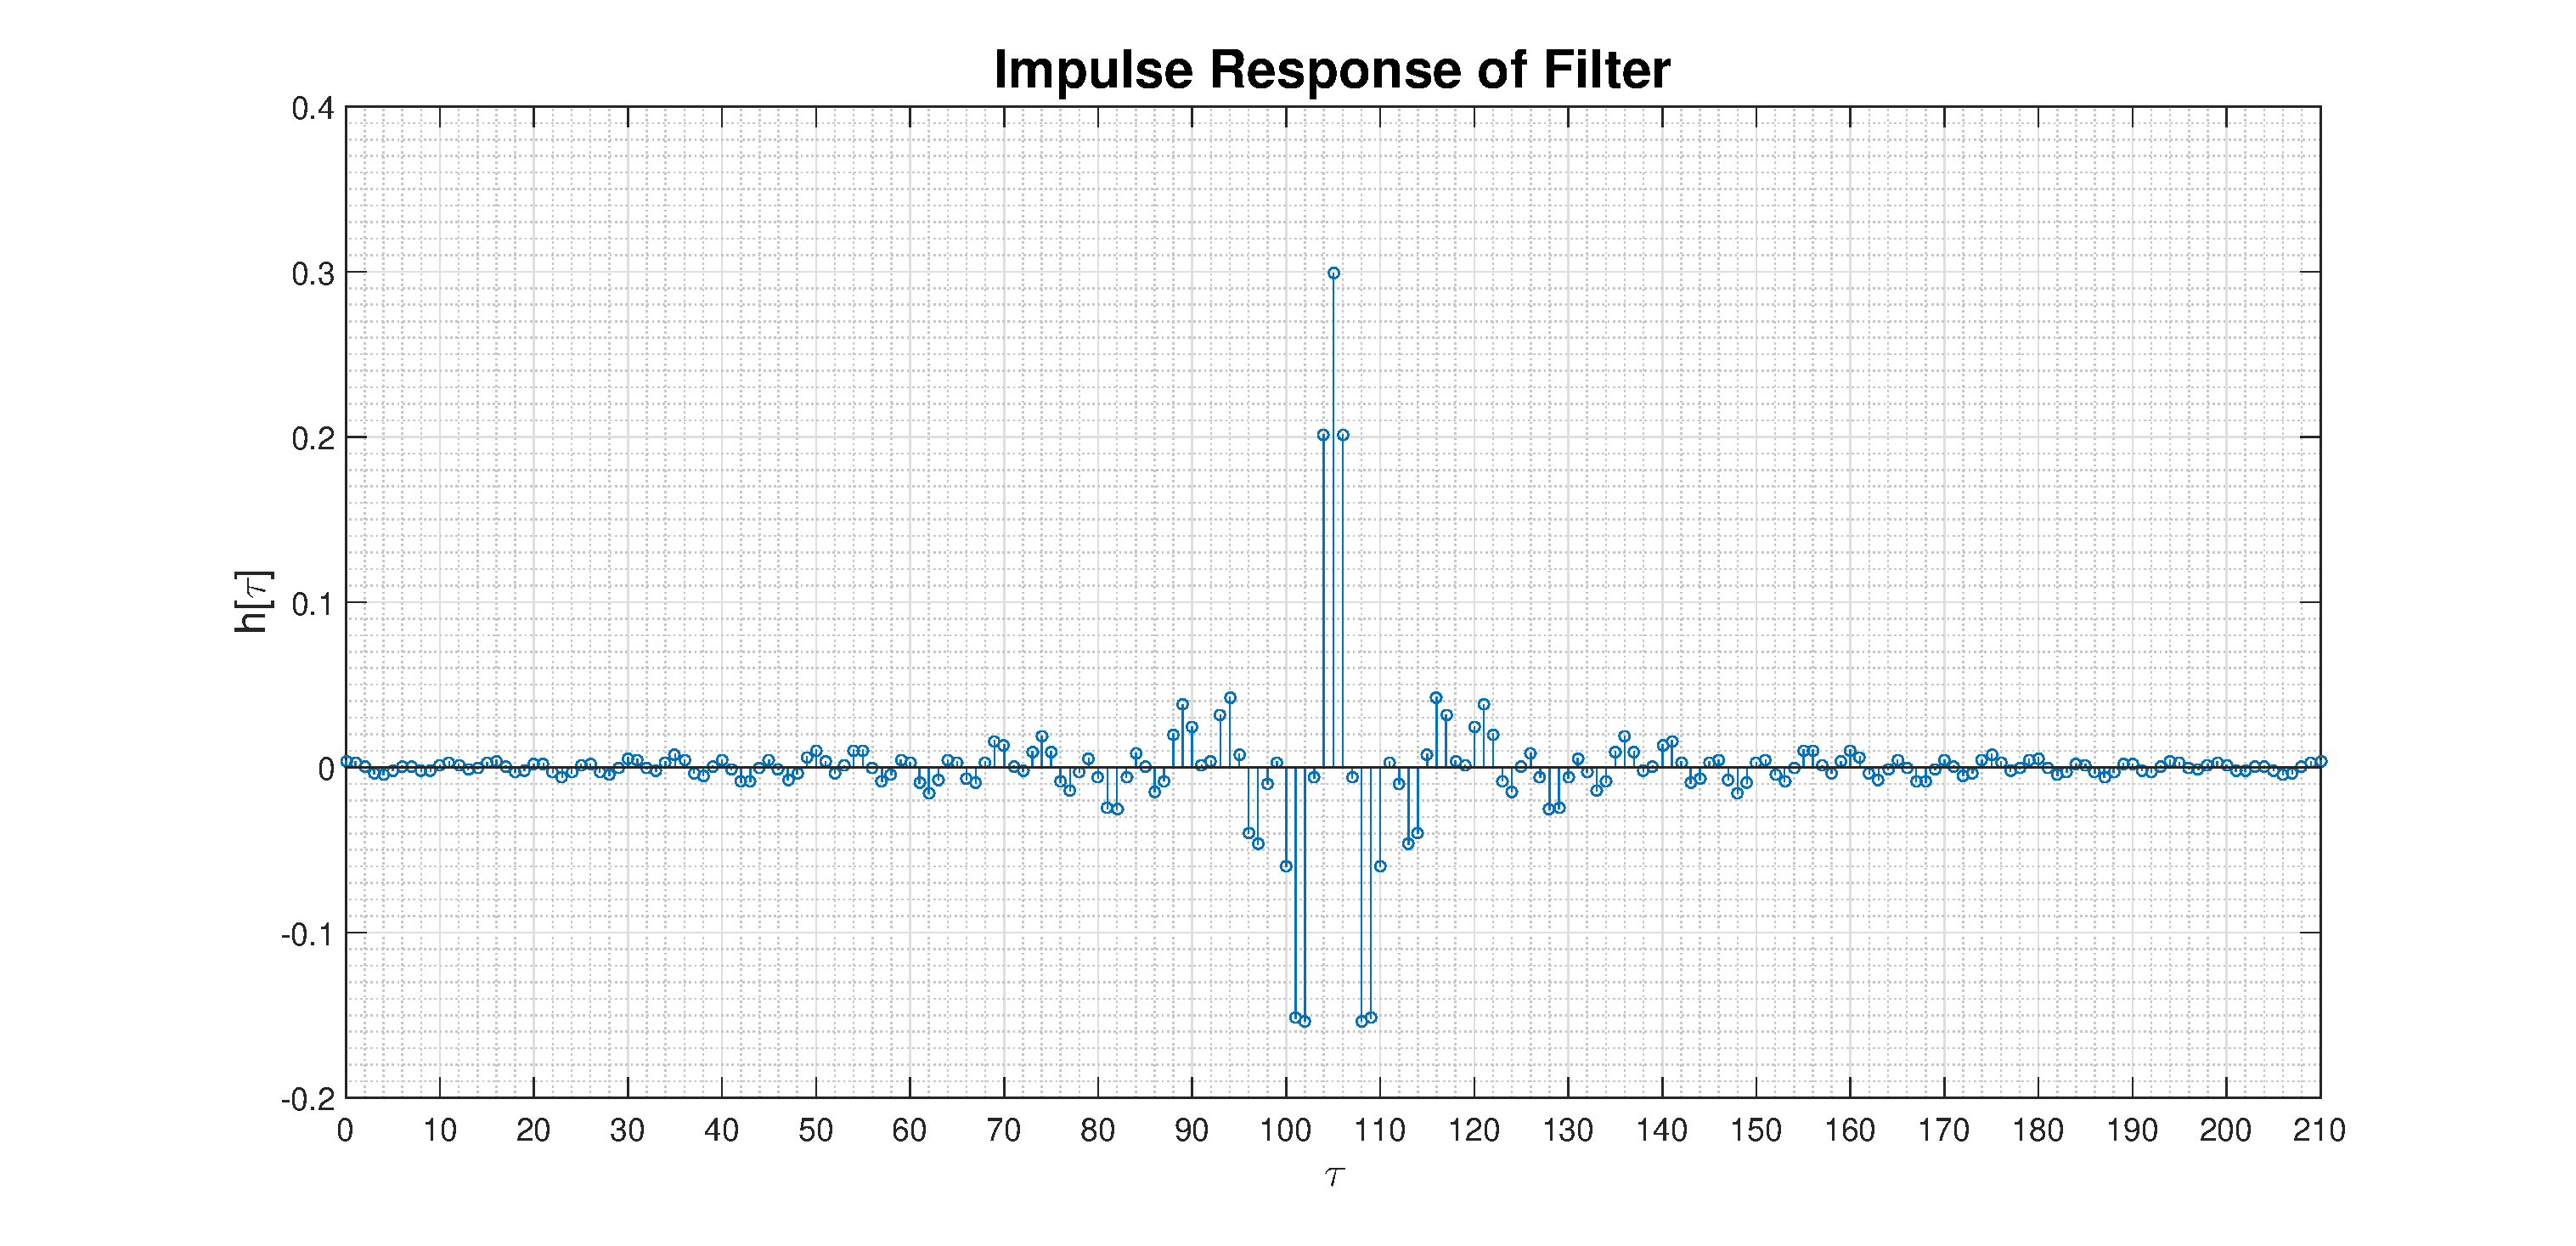
\includegraphics[width=0.49\textwidth]{impulse_response_filter_1}
    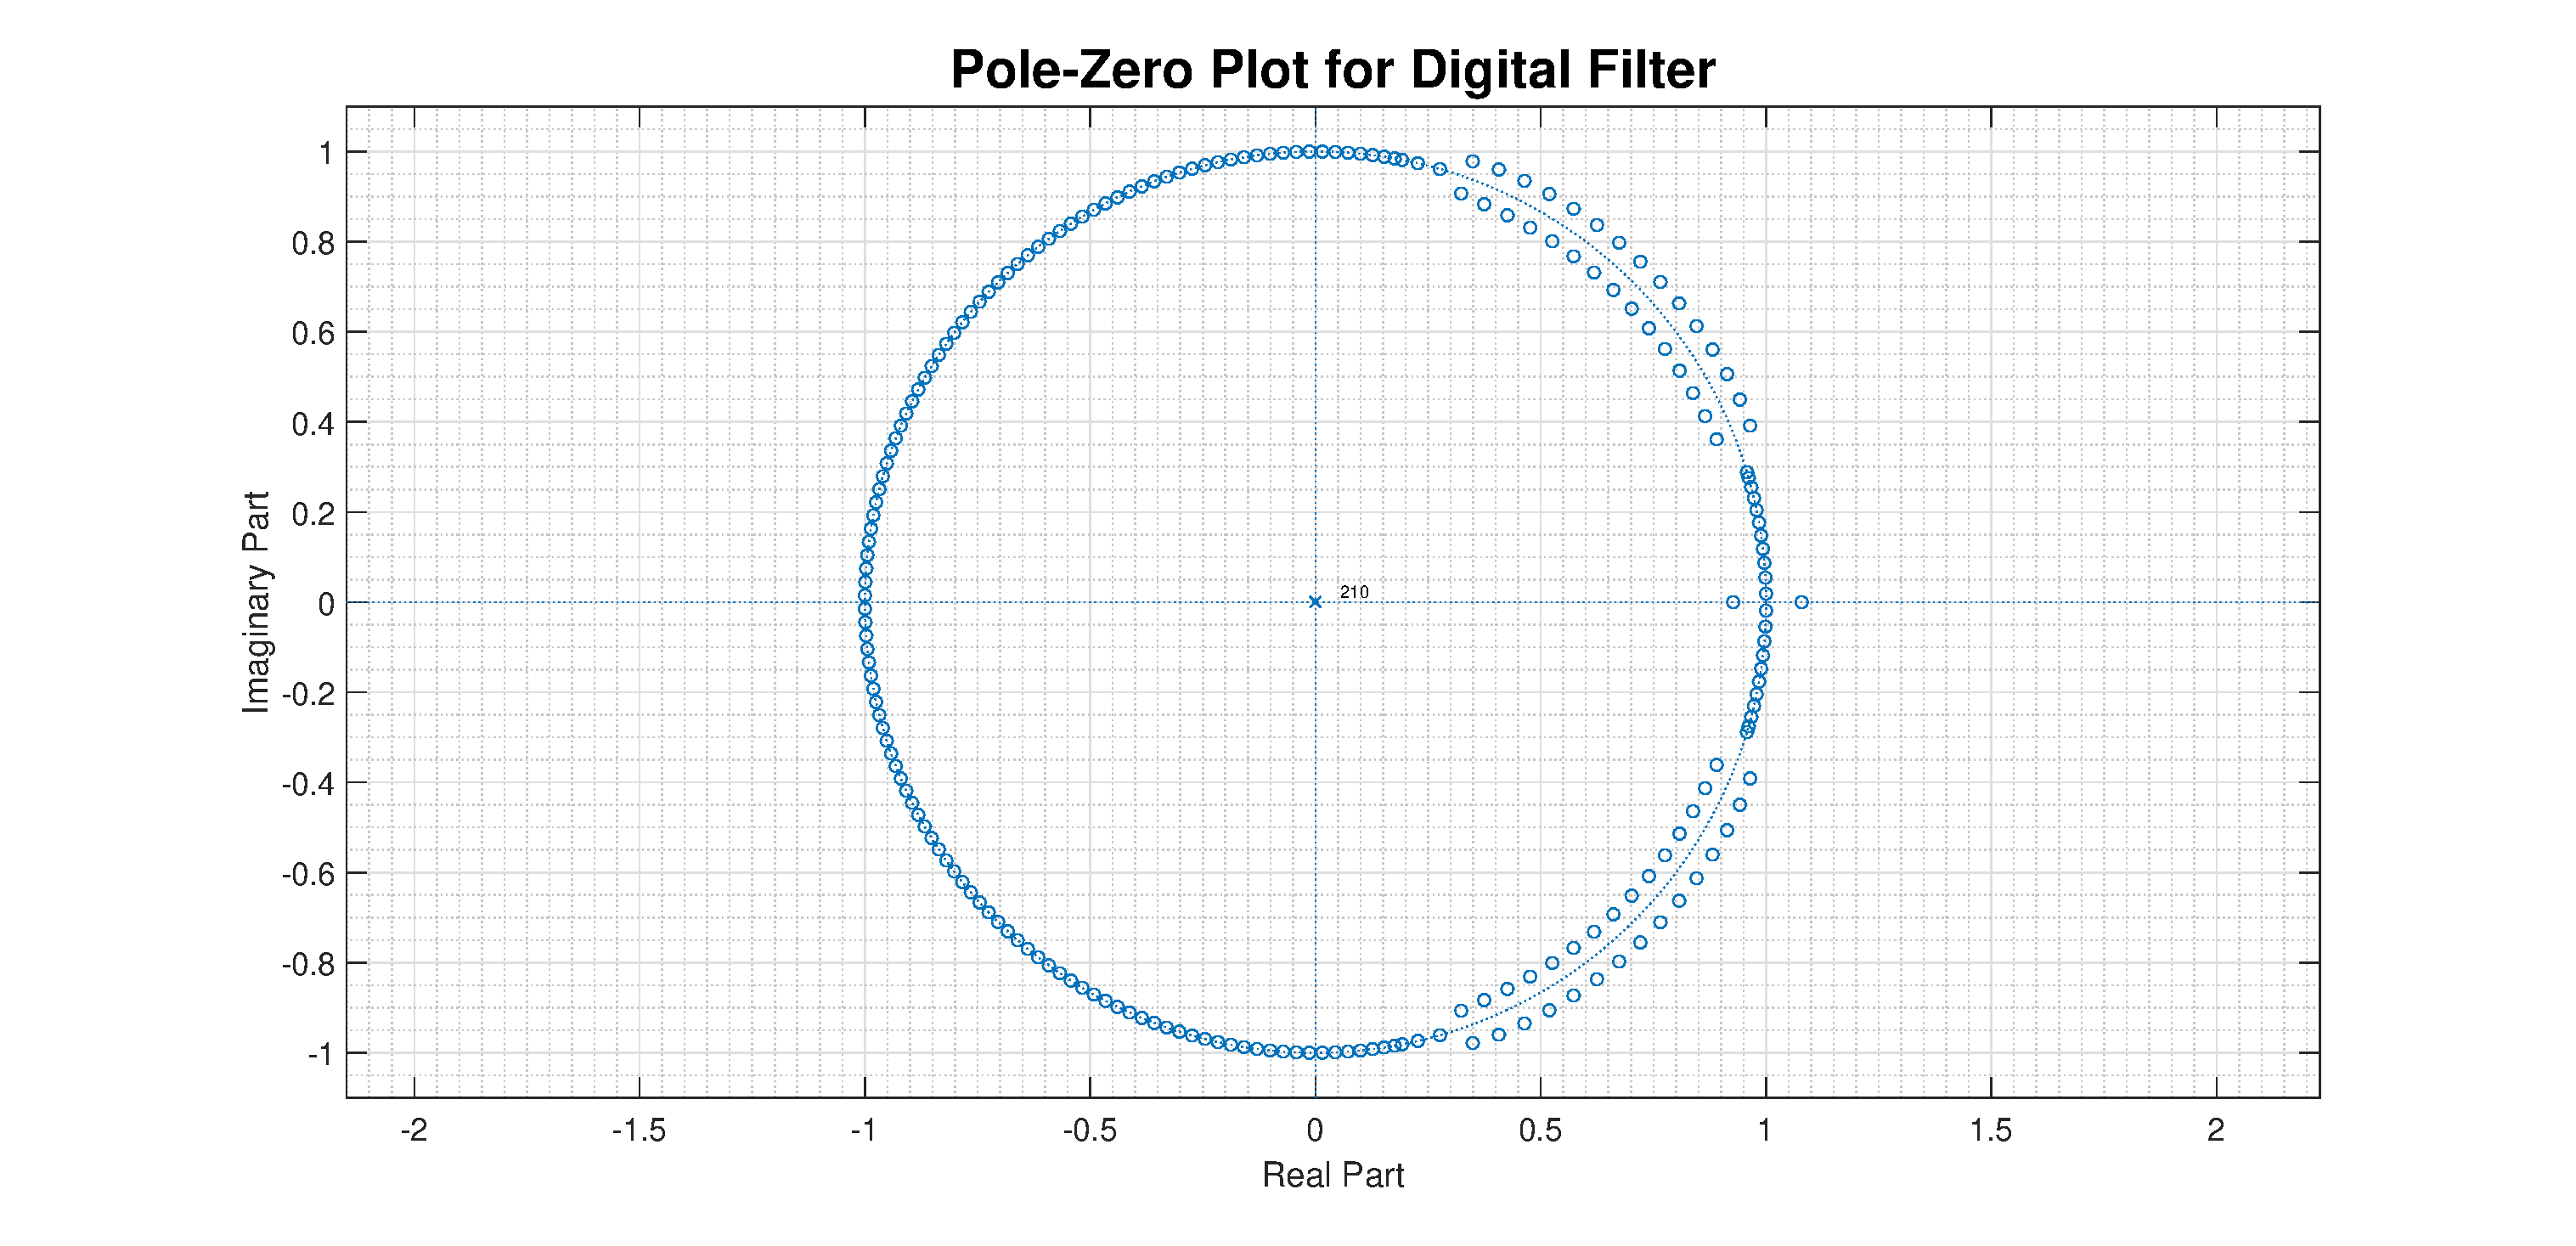
\includegraphics[width=0.49\textwidth]{pole_zero}
    \caption{Impulse response of designed filter}
    \label{fig:filter_coefs}
\end{figure}

To affirm that the filter meets all the specifications, specific frequencies are graphed in figure \ref{fig:filter_1_zooms}.

\begin{figure}[H]
    \centering
    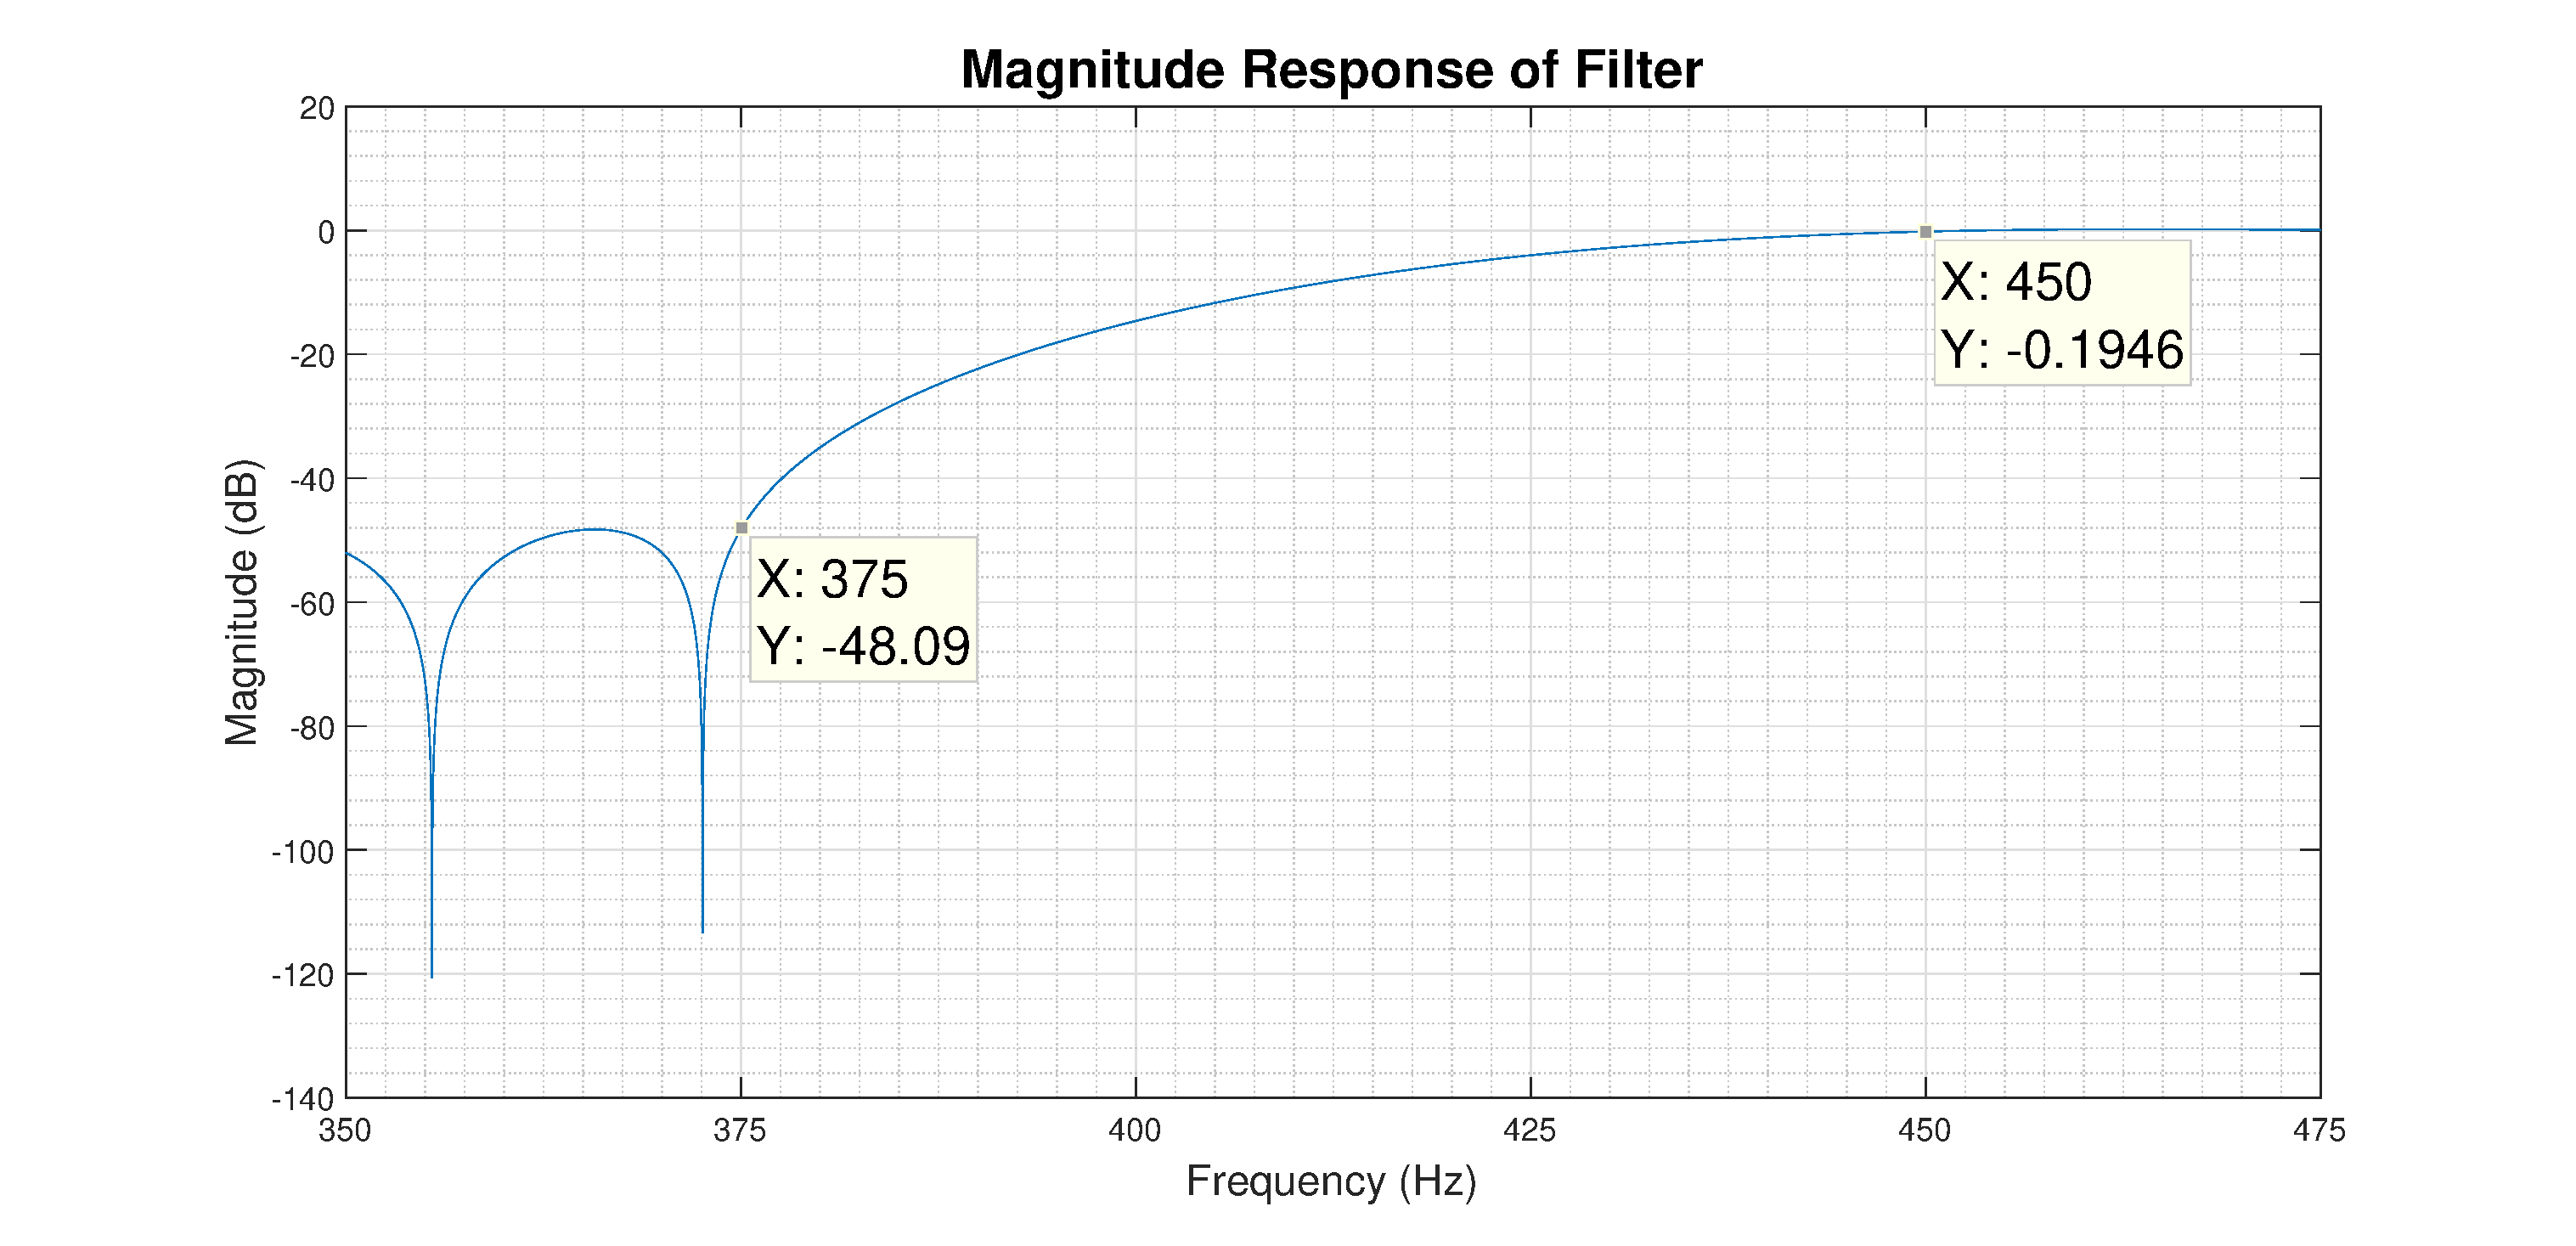
\includegraphics[width=0.42\textwidth]{filter_1_transition_1}\\
    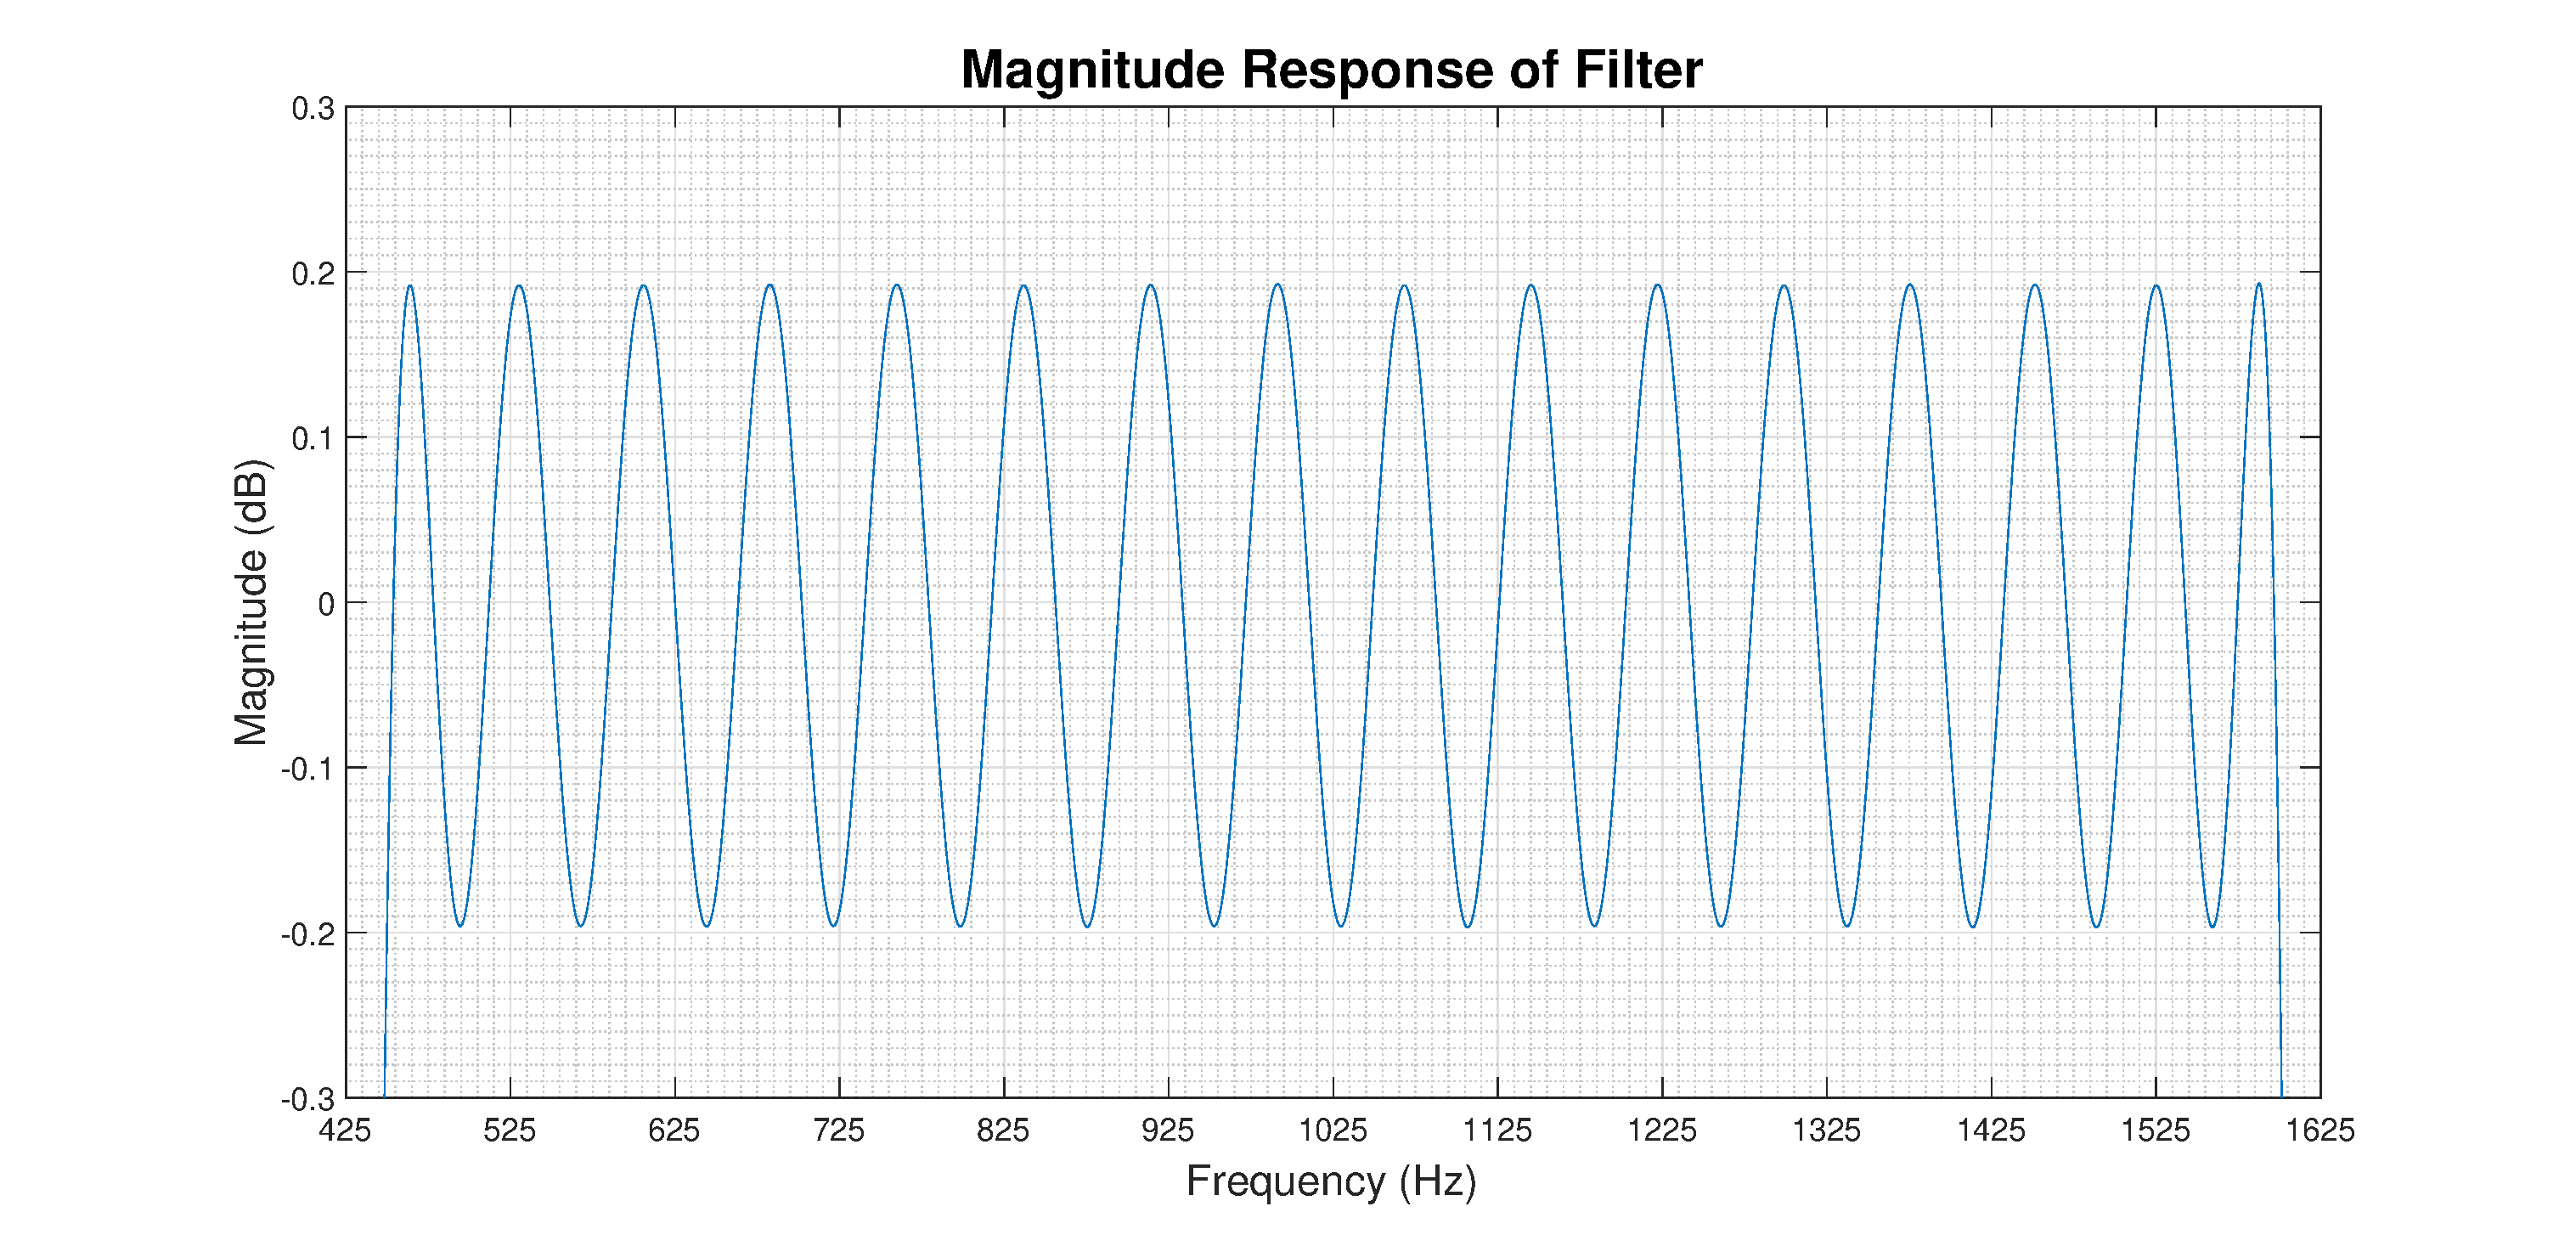
\includegraphics[width=0.42\textwidth]{filter_1_passband}\\
    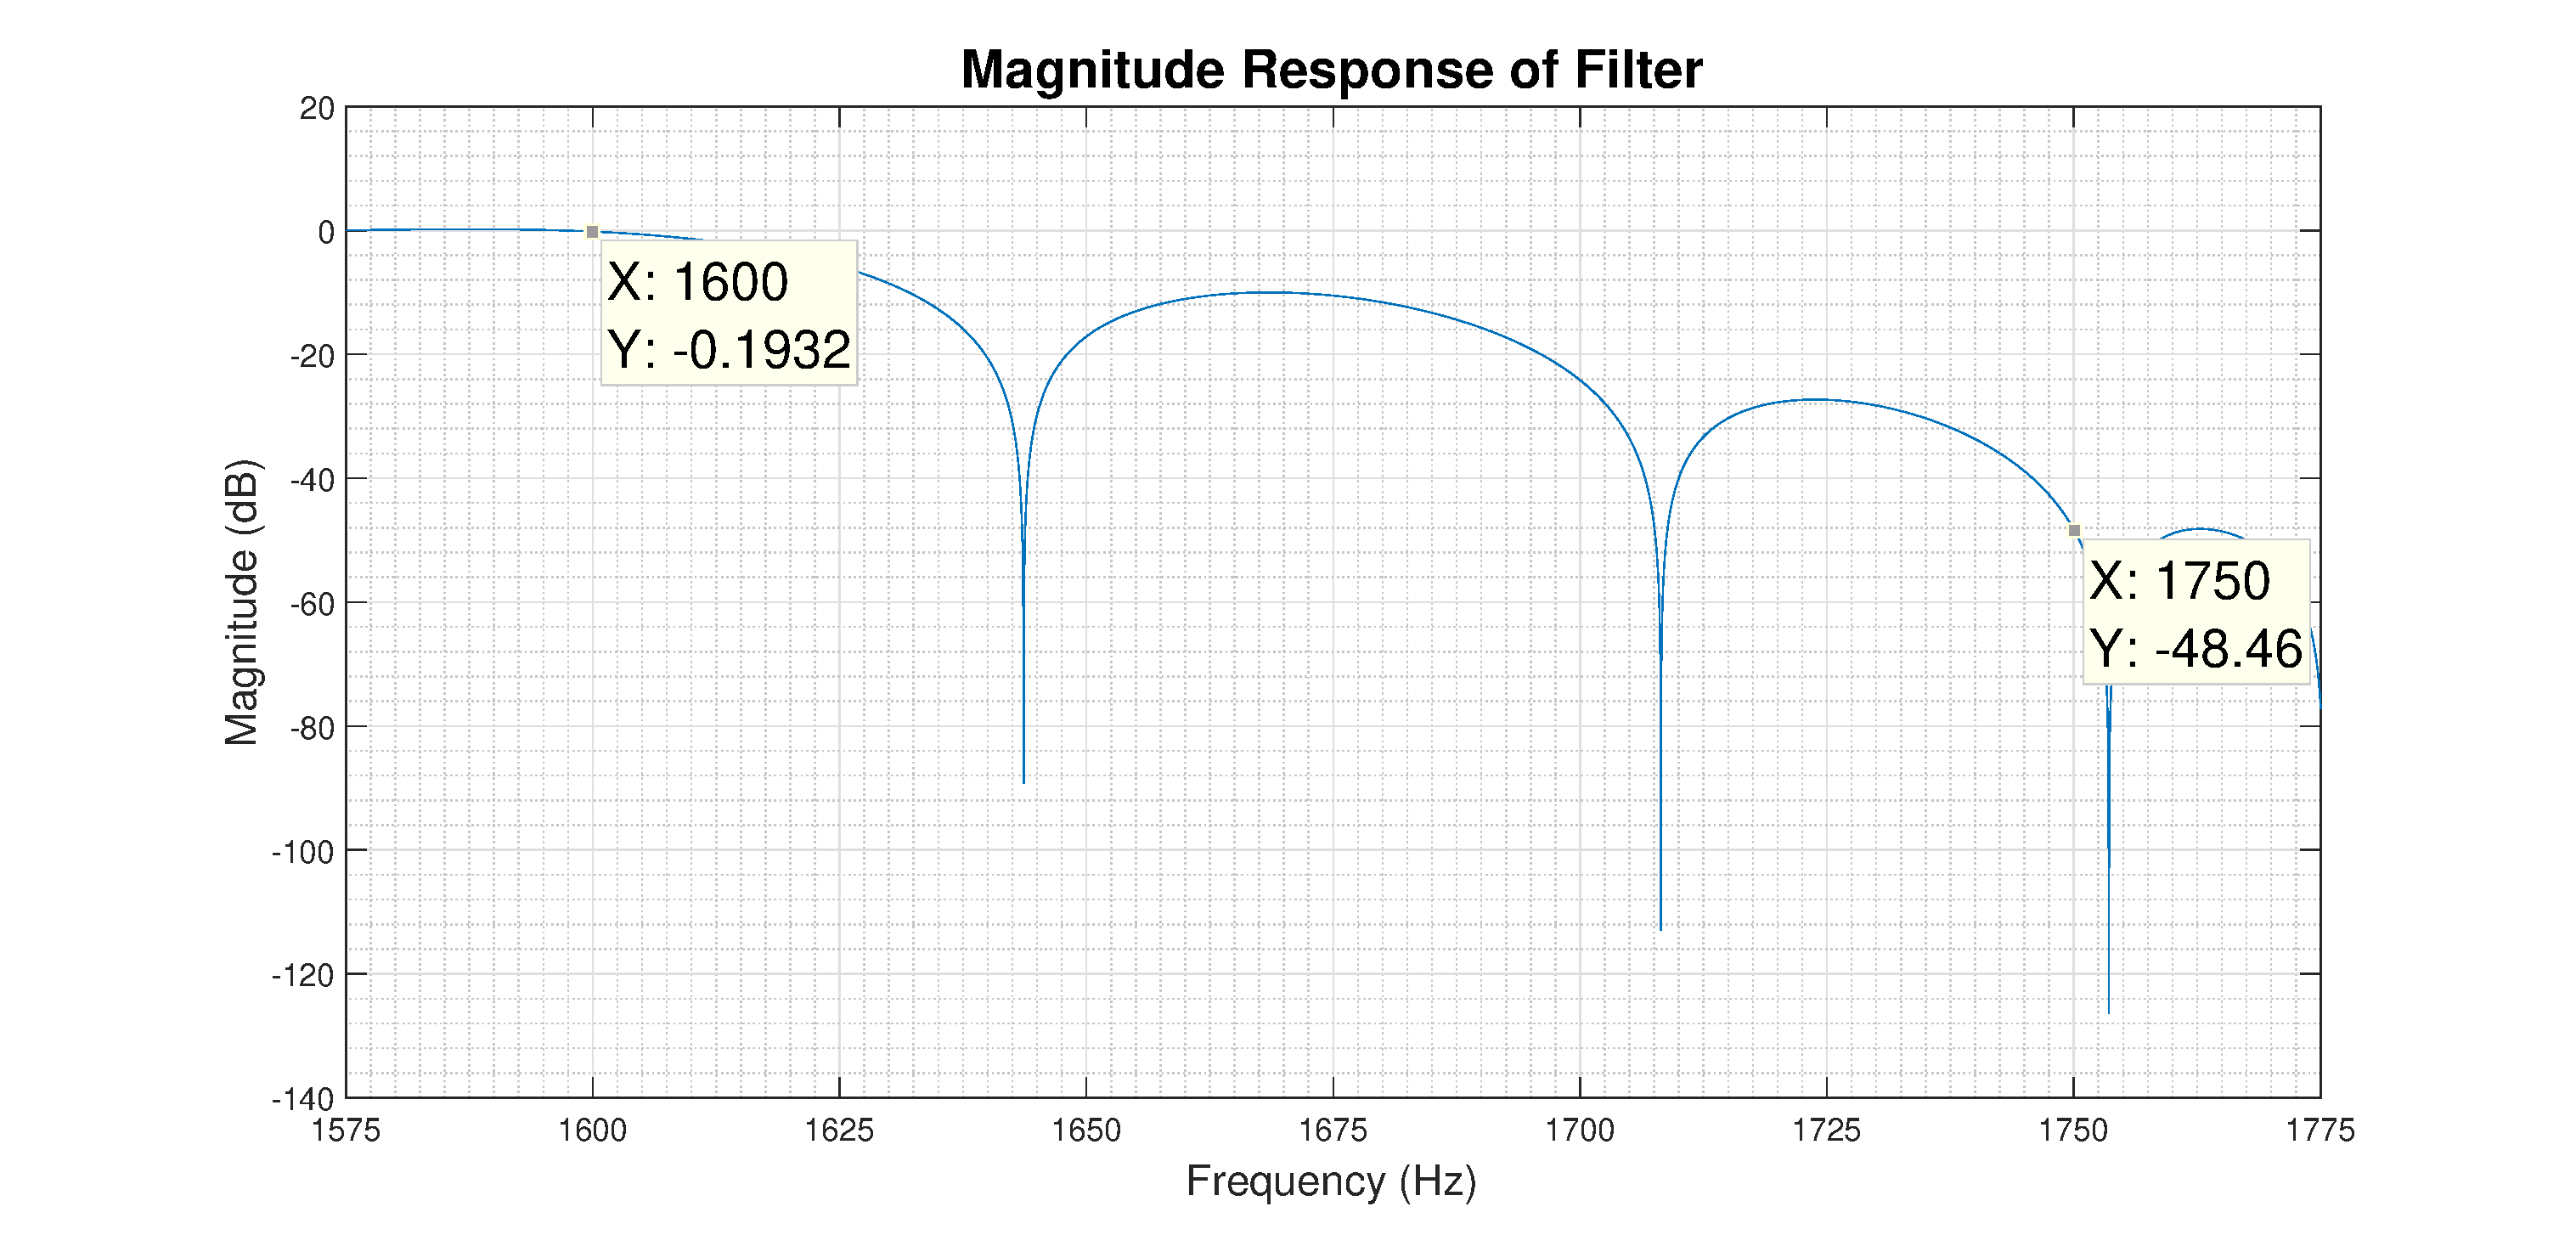
\includegraphics[width=0.42\textwidth]{filter_1_transition_2}
    \caption{Graphs showing that designed filter meets specifications}
    \label{fig:filter_1_zooms}
\end{figure}

\newpage
\section{FIR Filter Implementation: Non-Circular Buffering}
The first method of implementing the filter on the $TMS320C6713 \ DSK$ board is conceptually very simple. As discussed in section \ref{sec:FIR_theory}, a FIR filter of order $M$ will have a memory of $M$. This means that a buffer of size $M$ is required to keep track of the previous samples. In C, this buffer is implemented in the form of an array, {\tt x}. The output is calculated by computing the inner product of the filter coefficients, which are stored in array {\tt b}, and the past inputs as described in equation (\ref{eq:fir_diff_eq}).\\

\textbf{A simple buffer is implemented such that index of the array indicates the delay between the stored sample the current sample.} This is depicted in figure \ref{fig:simple_buffer}.\\

\begin{figure}[H]
\centering
\begin{tikzpicture}
 \foreach \c/\i [count=\n] in  
        {20/$x_{0}$,20/$x_{-1}$,20/$x_{-2}$} 
           \node[draw,minimum height=1cm,minimum width = 2cm,xshift=\n*2cm,font=\ttfamily](Si\n){\i};

  \node [tape, draw,minimum size=1cm,tape bend top=none,tape bend height=0.4cm,rotate=90] at (7.3,0) (t) {};
  \node [tape, draw,minimum size=1cm,tape bend top=none, tape bend height=0.4cm,rotate=270] at (9.3,0) (t) {};

\node (A) at (8.3,0.5) {\dots};
\node at (8.3,-0.5) {\dots};
\node[minimum height=1cm,minimum width = 2cm]  at (0,0) {$t=0$};


\foreach \c/\i [count=\m] in  
        {white!20/$x_{-M+1}$,white!20/$x_{-M}$} 
           \node[draw,fill=\c,minimum height=1cm,minimum width = 2cm,xshift=8.6cm+\m*2cm](Sj\m){\i} ;
           
\end{tikzpicture}
\caption{Simple Buffer}
\label{fig:simple_buffer}
\end{figure}

\textbf{To maintain the simplicity of this buffer requires a great deal of overhead.} Each time a new sample is read, every value in the array has to be shifted to the right. The shifting of the samples within the buffer is shown is figure \ref{fig:simple_buffer_shift}.\\

\begin{figure}[H]
\centering
\begin{tikzpicture}
    \foreach \c/\i [count=\n] in  {20/$x_{i}$,20/$x_{i-1}$,20/$x_{i-2}$} 
        \node[draw,minimum height=1cm,minimum width = 2cm,xshift=\n*2cm,yshift=3cm,font=\ttfamily](Ni\n){\i};
    
    \node [tape, draw,minimum size=1cm,tape bend top=none,tape bend height=0.4cm,rotate=90] at (7.3,3) (t) {};
    \node [tape, draw,minimum size=1cm,tape bend top=none, tape bend height=0.4cm,rotate=270] at (9.3,3) (t) {};
    
    \node at (8.3,3.5) {\dots};
    \node (B) at (8.3,2.5) {\dots};
    \node[minimum height=1cm,minimum width = 2cm]  at (0,3) {$t=t_{i}$};
    
    \foreach \c/\i [count=\m] in {white!20/$x_{i-(M-1)}$,white!20/$x_{i-M}$} 
        \node[draw,fill=\c,minimum height=1cm,minimum width = 2cm,xshift=8.6cm+\m*2cm,yshift=3cm,font=\ttfamily](Nj\m){\i} ;
    
    
    \foreach \c/\i [count=\n] in {20/$x_{i+1}$,20/$x_{i}$,20/$x_{i-1}$} 
        \node[draw,minimum height=1cm,minimum width = 2cm,xshift=\n*2cm,font=\ttfamily](Si\n){\i};
    
    \node [tape, draw,minimum size=1cm,tape bend top=none,tape bend height=0.4cm,rotate=90] at (7.3,0) (t) {};
    \node [tape, draw,minimum size=1cm,tape bend top=none, tape bend height=0.4cm,rotate=270] at (9.3,0) (t) {};
    
    \node (A) at (8.3,0.5) {\dots};
    \node at (8.3,-0.5) {\dots};
    \node[minimum height=1cm,minimum width = 2cm] at (0,0) {$t=t_{i}+1$};
    
    
    \foreach \c/\i [count=\m] in {white!20/$x_{(i+1)-(M-1)}$,white!20/$x_{(i+1)-M}$} 
        \node[draw,fill=\c,minimum height=1cm,minimum width = 2cm,xshift=8.6cm+\m*2cm](Sj\m){\i} ;
    
    \draw[my curvy arrow]  (Ni1.south) to (Si2.north);
    \draw[my curvy arrow]  (Ni2.south) to (Si3.north);
    \draw[my dashed curvy arrow]  (Ni3.south) to (A);
    \draw[my dashed curvy arrow]  (B) to (Sj1.north);
    \draw[my curvy arrow]  (Nj1.south) to (Sj2.north);

\end{tikzpicture}
\caption{Complete reorganisation of the buffer each time a new sample is read}
\label{fig:simple_buffer_shift}
\end{figure}

\textbf{Shifting of the buffer each time a new sample is read is computationally expensive.} Nonetheless, it is implemented in C and will form the baseline for performance analysis.

\begin{listing}[H]
\begin{minted}[fontsize=\scriptsize , linenos]{C}
void ISR_filter(void){			
    short sample_in;		
    int i;
    
    // newest sample is read into a temporary variable
    sample_in = mono_read_16Bit();		
    		
    // shifting of the buffer is performed
    for(i=M-1; i>0; i--)		
        x[i] = x[i-1];	
    
    // newest sample is moved from the temporary variable to its correct position in buffer
    x[0] = sample_in;
    
    // function that performs convolution is called
    // function returns a double and is converted to a short before being sent to output
    mono_write_16Bit((short)non_circ_FIR());		
}			

// function that performs convolution using a non-circular buffer			
double non_circ_FIR(void){			
    int i;		
    double y = 0;
    
    // inner product of array containing filter coefficients and buffer containing samples
    for(i=0; i<M; i++)
        y += b[i]*x[i];
	
    return y;		
}
\end{minted}
\caption{{\tt non\_circ\_FIR}}
\label{lst:non_circ_buffer}
\end{listing}

\subsection{Verification of Filter Implementation}
To ensure that the code in listing \ref{lst:non_circ_buffer} performs the filtering correctly, sine waves of different frequencies are used as inputs to test the frequency response\footnote{This is done for the sake of completion. In section \ref{sec:spec_analyser}, the spectrum analyser is used to check the frequency response of the filter}. Note that there are 2 analogue filters, 2 digital filters and a network of resistors on the board to prevent aliasing and adjust gains; these will result in attenuation.\textbf{ As such, the amplitude of input waves is kept constant such that relative changes in amplitude of the output waves are clear.} \\

The scope traces obtained are graphed in figure \ref{fig:low_freq_test}. The results are exactly expected. 
\begin{itemize}
    \item There is significant signal attenuation in the stop bands.
    \item The strength of the signal grows progressively in the transition band.
    \item There is slight variation in the peak-to-peak amplitude at different frequencies within the pass band. 
\end{itemize}

\begin{figure}[H]
    \centering
    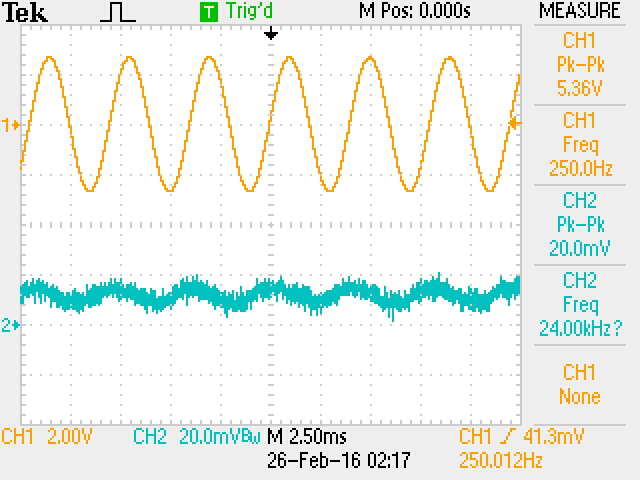
\includegraphics[width=0.32\textwidth]{250Hz}
    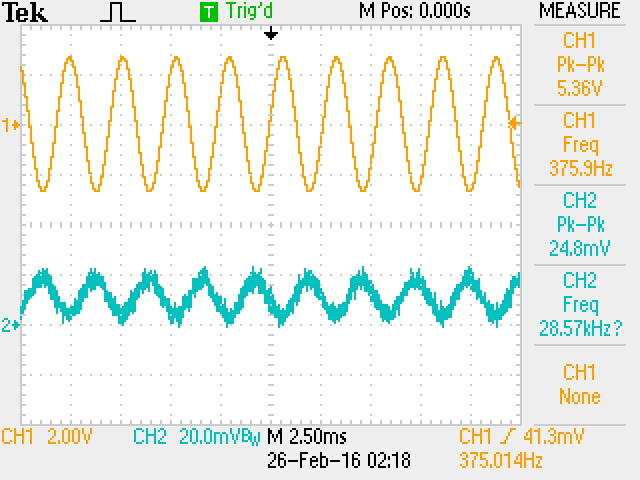
\includegraphics[width=0.32\textwidth]{375Hz}
    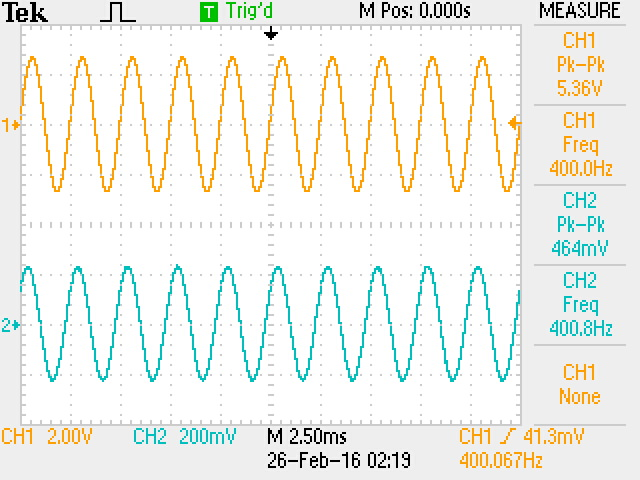
\includegraphics[width=0.32\textwidth]{400Hz}
    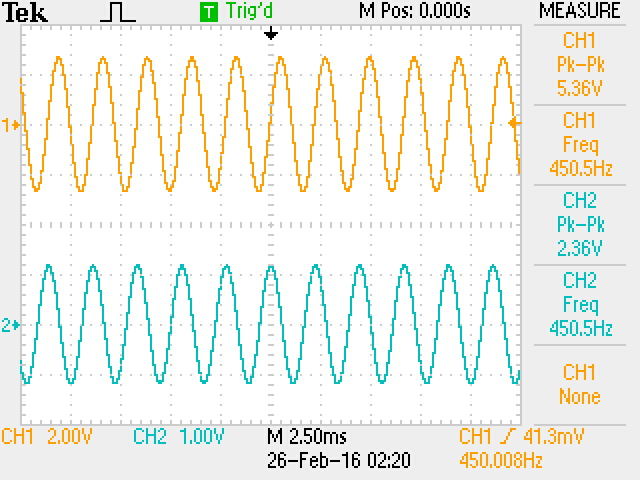
\includegraphics[width=0.32\textwidth]{450Hz}
    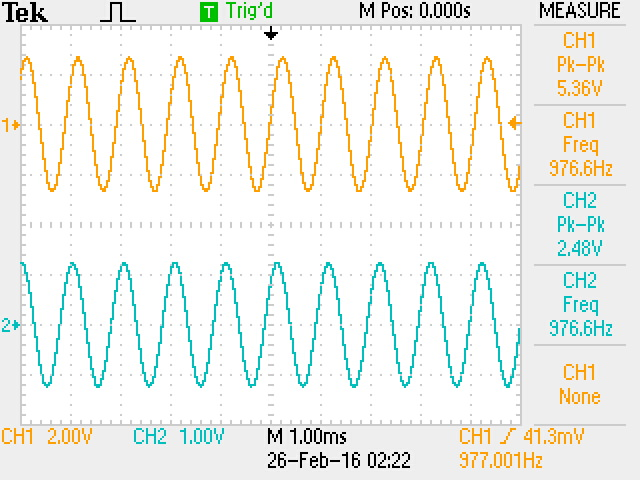
\includegraphics[width=0.32\textwidth]{977Hz}
    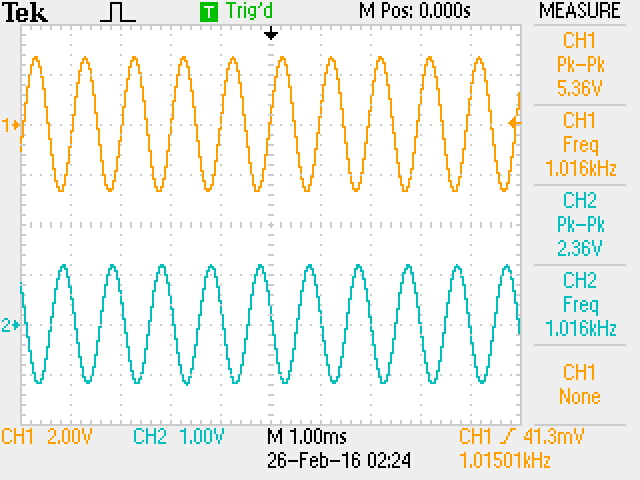
\includegraphics[width=0.32\textwidth]{1015Hz}
    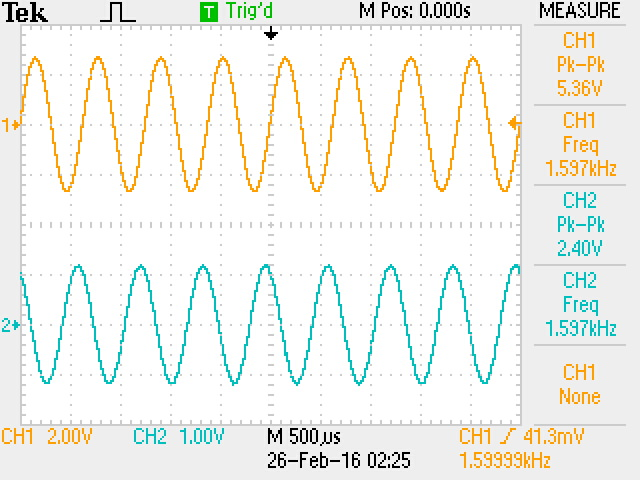
\includegraphics[width=0.32\textwidth]{1600Hz}
    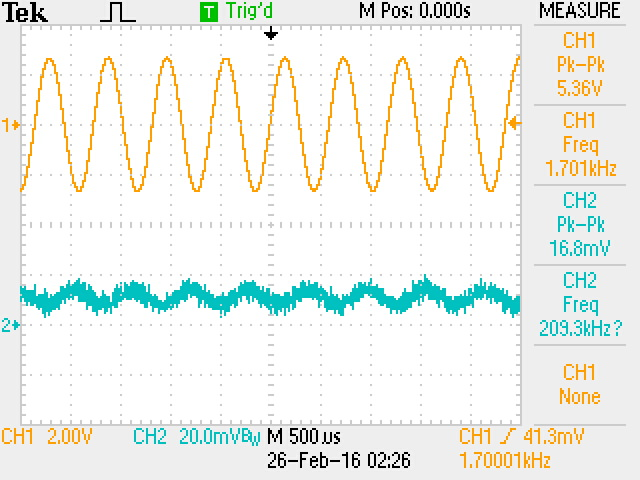
\includegraphics[width=0.32\textwidth]{1700Hz}
    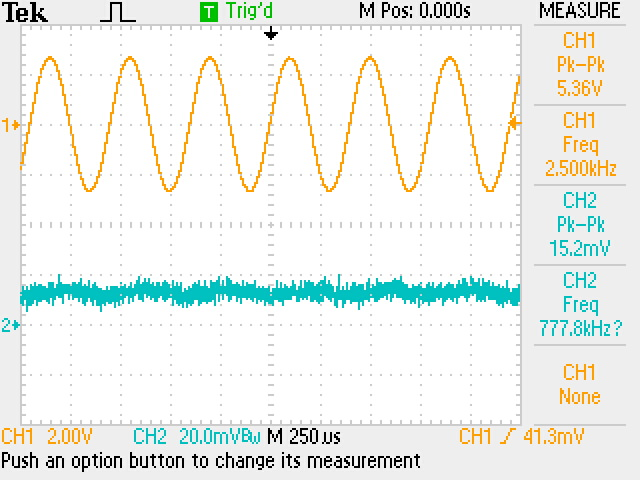
\includegraphics[width=0.32\textwidth]{2500Hz}
    \caption{Frequency spectrum analysis of filter}
    \label{fig:low_freq_test}
\end{figure}

\textbf{A detailed analysis of the frequency response is presented in section \ref{sec:spec_analyser}.}

\newpage
\section{FIR Filter Implementation: Circular Buffering}\label{sec:FIR_filter}
In this section, a more involved implementation of the buffer is explored. Previously, the index of the array represented the relative delay between the previous samples and the current sample. T\textbf{he array had a very regular structure and computing the inner product between the array containing the filter coefficients and the array containing the samples was simple.} Maintaining the regular structure of the array required a great deal of overhead as each iteration required complete reorganisation of the samples stored in the buffer.\\

Instead, a circular buffer is used. A variable {\tt ptr} keeps track of the index that the newest sample is stored in. \textbf{It is important to note that the variable {\tt ptr} is not an actual pointer, in that it does not contain a memory address; it is an integer that stores an array index.} New samples are placed to the left of older samples; the array grows towards {\tt x[0]} instead of towards {\tt x[M-1]}. When a new sample is read, it simply replaces the oldest sample in the buffer and the variable {\tt ptr} is decremented by $1$.\textbf{ This implementation is referred to as a circular buffer because the variable {\tt ptr} wraps around when it reaches the first element of the array.} This is clearly depicted in figure \ref{fig:circ_buffer_wrap}. For simplicity, a 6\textsuperscript{th} order filter is depicted.

\begin{figure}[H]
    \centering
    \begin{tikzpicture}
    \foreach \c/\i [count=\n] in  {20/$x_{i-4}$,20/$x_{i-5}$,20/$x_{i-6}$,20/$x_{i}$,20/$x_{i-1}$,20/$x_{i-2}$,20/$x_{i-3}$} 
        \node[draw,minimum height=1cm,minimum width = 2cm,xshift=\n*2cm,yshift=9cm,font=\ttfamily](N\n){\i};
        
    \node[minimum height=1cm,minimum width = 2cm] at (0,9) {$t=t_{i}$};    
    \node (A) at (8,7.5) {ptr};
    
    \draw[my arrow]  (A) to (N4.south);
    
    \foreach \c/\i [count=\n] in  {20/$x_{i-4}$,20/$x_{i-5}$,20/$x_{i+1}$,20/$x_{i}$,20/$x_{i-1}$,20/$x_{i-2}$,20/$x_{i-3}$} 
        \node[draw,minimum height=1cm,minimum width = 2cm,xshift=\n*2cm,yshift=6.5cm,font=\ttfamily](N\n){\i};
    
    \node[minimum height=1cm,minimum width = 2cm] at (0,6.5) {$t=t_{i}+1$};        
    \node (B) at (6,5) {ptr};
    
    \draw[my arrow]  (B) to (N3.south);
    
    \node (C) at (8,4) {$\vdots$};
    
     \foreach \c/\i [count=\n] in  {20/$x_{i+3}$,20/$x_{i+2}$,20/$x_{i+1}$,20/$x_{i}$,20/$x_{i-1}$,20/$x_{i-2}$,20/$x_{i+4}$} 
        \node[draw,minimum height=1cm,minimum width = 2cm,xshift=\n*2cm,yshift=2cm,font=\ttfamily](N\n){\i};
    
    \node[minimum height=1cm,minimum width = 2cm] at (0,2) {$t=t_{i}+4$};        
    \node (D) at (14,0.5) {ptr};
    
    \draw[my arrow]  (D) to (N7.south);
    
    \end{tikzpicture}
    \caption{Wrapping of {\tt ptr} in a circular buffer}
    \label{fig:circ_buffer_wrap}
\end{figure}

\textbf{The circular buffer requires significantly less overhead in terms of maintaining the structure of the buffer. This is however compensated by the increased complexity needed to implement the convolution sum.} An {\tt if} statement needs to be used to ensure that the variable {\tt ptr} does not exceed its bounds of $[0,M]$, where $M$ represents the filter order. To implement a filter of order $M$, $M+1$ coefficients and $M+1$ samples are necessary. This is clear from equation (\ref{eq:fir_diff_eq}). Thus, the variable {\tt ptr} can take $M+1$ distinct values. \\

An {\tt if} statement is also necessary when reading data into the buffer.

\newpage
Listing \ref{lst:simple_cir} shows the code required to implement the circular buffer in C. \textbf{Updating of the buffer and all read and write operations are performed in {\tt ISR\_filter} whereas {\tt circ\_FIR} only performs the convolution sum and returns the result.} Separating the two distinct tasks into unique functions makes for increased readability. The overhead of making function calls within the ISR is eliminated at compile time\footnote{More details about compiler optimisations are provided in section \ref{sec:com_opt}.}.\\

\begin{listing}[H]
\label{lst:simple_cir}
\begin{minted}[fontsize=\scriptsize, linenos]{C}
void ISR_filter(void){
    
    // new sample is stored directly into the buffer
    x[ptr] = mono_read_16Bit();		
    
    // function that performs convolution is called
    // function returns a double and is converted to a short before being sent to output
    mono_write_16Bit((short)circ_FIR());
    
    // updates the position of the pointer
    ptr--;		
    
    // checks if the ptr needs to be wrapped around
    if(ptr<0)	
        ptr = M-1;	

}			
			
double circ_FIR(void){			
    short i;		
    double y = 0;		
    
    // inner product of array containing filter coefficients and buffer containing samples
    // after M iterations, the value of ptr is unchanged
    for(i=0; i<M; i++){		
        y += b[i]*x[ptr];	
        ptr--;
        
        // checks if the ptr needs to be wrapped around
        if(ptr<0)	
            ptr = M-1;
    }		
    
    return y;		
}			
\end{minted}
\caption{{\tt circ\_FIR}}
\end{listing}

\newpage
\section{FIR Filter Implementation: Circular Buffering Exploiting Symmetry}\label{sec:exploit_symmetry}
\subsection{Function that Uses {\tt if} Statements}\label{sec:if_statement_code}
As mentioned in section \ref{sec:FIR_theory}, a FIR filter is usually implemented when a linear phase response is required. A linear phase response can by achieved by placing zeroes to produce a symmetric impulse response. The symmetric relationship between coefficients of a linear phase FIR filter is stated in equation (\ref{eq:symmetric}) and figure \ref{fig:filter_coefs} corroborates the fact that the designed filter's coefficients are indeed symmetric. \textbf{This symmetry can be exploited to halve the number of multiplication operations that need to be computed to perform filtering. Since pairs of samples are going to be multiplied by the same coefficient, the samples can first be added, then multiplied.} This is depicted in the block diagram shown in figure \ref{fig:fir_symmetric_signal_flow}.\\   

Computationally, this implementation provides a significant improvement since the {\tt for} loop\footnote{Number of multiplies per iteration of the {\tt for} loop is constant. There is only one multiply operation per iteration.} required to compute the convolution sum only needs $\nicefrac{M-1}{2}$ iterations. However, for correct implementation, two pointers\footnote{Again it is key to note that the term pointer is used loosely. In fact, two variables defined as integers are created and used to keep track of two distinct positions in the buffer.} need to be managed. One pointer will traverse the samples in the order $x_{0}$, $x_{-1}$, $\cdots$, whereas the other pointer will traverse the samples in the order $x_{-M}$, $x_{-M+1}$, $\cdots$. 
\begin{itemize}
    \item \textbf{The first pointer is called {\tt move\_right} and initialised to be equal to {\tt ptr}.}
    \item \textbf{The second pointer is called {\tt move\_left} and initialised to be equal to ${\tt ptr}-1$.}
\end{itemize}

\textbf{This improved implementation also utilises the circular buffer and thus it has a similar flaw; there is a potential of the pointers going out of range.} Unless the initial position of {\tt ptr} is right in the middle of the buffer {\tt x}, either {\tt move\_right} or {\tt move\_left} will reference an invalid memory location at a certain iteration of the {\tt for} loop. This needs to be dealt with, in a similar manner to that presented in listing \ref{lst:simple_cir}, with the use of {\tt if} statements. \textbf{Both pointers do not need to be checked at every iteration of the for loop because each time the function {\tt circ\_FIR\_symmetric} is called, only one of the pointers will overflow.} The list below summarises which initial condition will lead to which pointer overflowing. 
\begin{itemize}
    \item \textbf{${\tt ptr} \leq \nicefrac{M-1}{2}$: {\tt move\_left} will overflow}
    \item \textbf{${\tt ptr} \geq \nicefrac{M-1}{2}$: {\tt move\_right} will overflow}
    \item \textbf{${\tt ptr} = \nicefrac{M-1}{2}$: neither {\tt move\_left} nor {\tt move\_right} will overflow}
\end{itemize}

The case where ${\tt ptr} \leq \nicefrac{M-1}{2}$ is depicted in figure \ref{fig:circ_overflow}. 

\begin{figure}[H]
    \centering
    \begin{tikzpicture}
    \foreach \c/\i [count=\n] in  {20/$x_{i-6}$,20/$x_{i}$,20/$x_{i-1}$,20/$x_{i-2}$,20/$x_{i-3}$,20/$x_{i-4}$,20/$x_{i-5}$} 
        \node[draw,minimum height=1cm,minimum width = 2cm,xshift=\n*2cm,yshift=9cm,font=\ttfamily](N\n){\i};
        
    \node[minimum height=1cm,minimum width = 2cm] at (0,9) {$Initial$};    
    \node (A) at (4,7.5) {ptr};
    
    \draw[my arrow]  (A) to (N2.south);
    
    \foreach \c/\i [count=\n] in  {20/$x_{i-6}$,20/$x_{i}$,20/$x_{i-1}$,20/$x_{i-2}$,20/$x_{i-3}$,20/$x_{i-4}$,20/$x_{i-5}$} 
        \node[draw,minimum height=1cm,minimum width = 2cm,xshift=\n*2cm,yshift=6.5cm,font=\ttfamily](N\n){\i};
        
    \node[minimum height=1cm,minimum width = 2cm] at (0,6.5) {$i=0$};    
    \node (B) at (2,5) {move\_left};
    \node (C) at (4,5) {move\_right};
    
    \draw[my arrow]  (B) to (N1.south);
    \draw[my arrow]  (C) to (N2.south);
    
     \foreach \c/\i [count=\n] in  {20/$x_{i-6}$,20/$x_{i}$,20/$x_{i-1}$,20/$x_{i-2}$,20/$x_{i-3}$,20/$x_{i-4}$,20/$x_{i-5}$} 
        \node[draw,minimum height=1cm,minimum width = 2cm,xshift=\n*2cm,yshift=4cm,font=\ttfamily](N\n){\i};
        
    \node[minimum height=1cm,minimum width = 2cm] at (0,4) {$i=1$};    
    \node (D) at (14,2.5) {move\_left};
    \node (E) at (6,2.5) {move\_right};
    
    \draw[my red arrow]  (D) to (N7.south);
    \draw[my arrow]  (E) to (N3.south);
    
    \end{tikzpicture}
    \caption{{\tt move\_left} will overflow before {\tt move\_right}}
    \label{fig:circ_overflow}
\end{figure}

\newpage
\textbf{Thus, if the initial position of the variable {\tt ptr} is checked, only one pointer will overflow and only one {\tt if} statements is needed in the {\tt for} loop.} Listing \ref{lst:circ_FIR_symmetric} presents the code that is used to implement a linear phase FIR filter by exploiting the symmetric nature of the impulse response. \textbf{Note that, the filter designed in MATLAB has an odd number of coefficients and thus one multiply accumulate step is implemented outside the {\tt for} loop.}

\begin{listing}[H]
\begin{minted}[fontsize=\scriptsize,linenos]{C}
// symmetry of linear phase FIR filter is exploited
// elements are added before multiply
// filter has odd number of coefficients, last term calculated separately
double circ_FIR_symmetric(void){
    int i;
    int move_right =  ptr;			
    int move_left = ptr - 1;			
    double y = 0;				
    
    // special case that move_left initialised to element not in the array				
    if(move_left == -1)				
        move_left = M-1;			
    
    // move_left will go out of range before move_right 
    if(ptr<(M-1)/2){
        for(i=0; i<(M-1)/2; i++){	
            y += b[i]*(x[move_left]+x[move_right]);	
            
            // incrementing move_right without checking since there is no danger of overflow
            move_right++;
            
            // move_left needs to be checked before decrementing, can go out of bounds
            if(move_left<=0)		
                move_left = M-1;	
            else		
                move_left--;	
        }		
        y += b[(M-1)/2]*x[move_right];			
    }
    // move_right will go out of range before move_left
    else if(ptr>(M-1)/2){
        for(i=0; i<(M-1)/2; i++){
            y += b[i]*(x[move_left]+x[move_right]);		
            
            // decrementing move_left without checking since there is no danger of overflow
            move_left--;
            
            // move_right needs to be checked before incrementing, can go out of bounds
            if(move_right>=M-1)		
                move_right = 0;	
            else		
                move_right++;	
        }
        y += b[(M-1)/2]*x[move_left];			
    }
    // neither move_right nor move_left will go out of bound
    else{
        for(i=0; i<(M-1)/2; i++){
            y+= b[i]*(x[move_left]+x[move_right]);		
        
            // neither move_left nor move_right needs to be checked
            move_left--;		
            move_right++;		
        }
        y += b[(M-1)/2]*x[move_right];			
    }
    return y;
}
\end{minted}
\caption{{\tt circ\_FIR\_symmetric}}
\label{lst:circ_FIR_symmetric}
\end{listing}

\subsection{Function that Completely Eliminates the Use of {\tt if} Statements}
Next, it is possible to completely eliminate the use of {\tt if} statements from the C code. As described in section \ref{sec:if_statement_code}, only one of the pointers, either {\tt move\_left} or {\tt move\_right} will overflow during the {\tt for} loop used to compute the convolution sum. \textbf{It is possible to calculate the number of iterations before the pointers will overflow using the value of {\tt ptr}.} The list below summarises this argument.
\begin{itemize}
    \item \textbf{${\tt ptr} \leq \nicefrac{M-1}{2}$: {\tt move\_left} will overflow after {\tt ptr} iterations, where {\tt ptr} is an integer within the range $[0,\nicefrac{M-1}{2}]$}
    \item \textbf{${\tt ptr} \geq \nicefrac{M-1}{2}$: {\tt move\-right} will overflow after $M-{\tt ptr}$ iterations, where $M-{\tt ptr}$ is an integer within the range $[1,\nicefrac{M-1}{2}]$}
    \item \textbf{${\tt ptr} \geq \nicefrac{M-1}{2}$: neither {\tt move\_left} nor {\tt move\_right} will overflow} 
\end{itemize}
\textbf{Note that, in case $1$, {\tt move\_left} can overflow even before the {\tt for} loop begins. This special case will be dealt with separately.\\}

Listing \ref{lst:two_for_loops} provides the C code that implements a FIR linear phase filter without the use of any {\tt if} statements. There are several things that should be noted for the code below:
\begin{itemize}
    \item {\tt move\_left++} and {\tt move\_right--} are used to reduce the amount of code required.
    \item In between the two {\tt for} loops, the pointer that overflows is wrapped around.
    \item Again, because the number of filter coefficients is odd, one multiply accumulate step is implemented outside the {\tt for} loops.
\end{itemize}

\begin{listing}[H]
\begin{minted}[fontsize=\scriptsize,linenos]{C}
// two for statements are used to eliminate the use of if statements
double circ_FIR_two_for_loops(void){					
    int i;				
    double y = 0;
    int end;	
    int move_right = ptr;
    int move_left = ptr-1;
    
    // special case, ptr points to the first element
    if(ptr==0){
        // wrap left pointer around
        move_left = M-1;
        
        for(i=0; i<(M-1)/2;i++)			
            y+= b[i]*(x[move_left--]+x[move_right++]);
        
        y+= b[(M-1)/2]*x[(M-1)/2];			
    }
    // left moving point will go out of bounds
    else if(ptr<(M-1)/2){
        // calculate the number of iterations for the first loop
        end = ptr;
        
        for(i=0; i<end; i++)			
            y += b[i]*(x[move_left--]+x[move_right++]);
        
        move_left = M - 1;
        
        // second for loop accounts for the overflow
        for(i=end; i<(M-1)/2;i++)			
            y += b[i]*(x[move_left--]+x[move_right++]);		
        
        y += b[(M-1)/2]*x[ptr+(M-1)/2];			
    }
    // right moving point will go out of bounds
    else if(ptr>(M-1)/2){
        // calculate the number of iterations for the first loop
        end = M-ptr;
        
        for(i=0; i<end; i++)			
            y += b[i]*(x[move_left--]+x[move_right++]);
        
        move_right = 0;
        
        // second loop accounts for the overflow
        for(i=end; i<(M-1)/2;i++)			
            y += b[i]*(x[move_left--]+x[move_right++]);		
        
        y += b[(M-1)/2]*x[ptr-1-(M-1)/2];			
    }
    // neither left moving pointer, nor right moving pointer overflows
    else{
        for(i=0; i<(M-1)/2; i++)			
            y+= b[i]*(x[move_left--]+x[move_right++]);	
            
        y += b[(M-1)/2]*x[M-1];			
    }				
    return y;				
}
\end{minted}
\caption{{\tt circ\_FIR\_two\_for\_loops}} 
\label{lst:two_for_loops}
\end{listing}


\newpage
\section{FIR Filter Implementation: Circular Buffering with Doubled Memory Size}
Up until this point, filter implementation has been improved by:
\begin{itemize}
    \item Using a circular buffer
    \item Exploiting the symmetry of the impulse response 
\end{itemize}
Using the circular buffer significantly increases the efficiency of the program however, there is a possibility of overflow which has to be accounted for. An overflow can occur both when reading new samples into the array as well as computing the inner product between the array containing the samples and the array containing the filter coefficients. \textbf{Overflow during the inner product can be avoided if a buffer of size $2M$ instead of size $M$.} This implementation does have overhead costs:
\begin{itemize}
    \item \textbf{Buffer of size $2M$ instead of $M$ is needed}
    \item \textbf{New sample needs to be read into two positions instead of just one; positions are offset by M}
\end{itemize}

This implementation is illustrated in figure \ref{fig:double_mem_buff}.
 
\begin{figure}[H]
    \centering
    \begin{tikzpicture}
    \foreach \c/\i [count=\n] in  {20/$x_{i-2}$,20/$x_{i-3}$,20/$x_{i}$,20/$x_{i-1}$,20/$x_{i-2}$,20/$x_{i-3}$,20/$x_{i}$,20/$x_{i-1}$} 
        \node[draw,minimum height=1cm,minimum width = 2cm,xshift=\n*2cm,yshift=9cm,font=\ttfamily](N\n){\i};
        
    \node (A) at (6,7.5) {ptr};
    \node (B) at (14,7.5) {ptr+M};
    
    \draw[my arrow]  (A) to (N3.south);
    \draw[my arrow]  (B) to (N7.south);
    
    \foreach \c/\i [count=\n] in  {20/$x_{i-2}$,20/$x_{i-3}$,20/$x_{i}$,20/$x_{i-1}$,20/$x_{i-2}$,20/$x_{i-3}$,20/$x_{i}$,20/$x_{i-1}$} 
    \node[draw,minimum height=1cm,minimum width = 2cm,xshift=\n*2cm,yshift=6.5cm,font=\ttfamily](N\n){\i};
        
    \node (A) at (6,5) {move\_right};
    \node (B) at (12,5) {move\_left};
    
    \draw[my arrow]  (A) to (N3.south);
    \draw[my arrow]  (B) to (N6.south);
    
    \end{tikzpicture}
    \caption{Circular buffer of size $2M$}
    \label{fig:double_mem_buff}
\end{figure}

Listing \ref{lst:double_buff} shows the C code that implements the linear phase FIR filter using a buffer of size $2M$. Again {\tt move\_left++} and {\tt move\_right--} are used to reduce the amount of code required. \textbf{Also, note that {\tt move\_left} is initialised to ${\tt ptr}+M-1$. }

\begin{listing}[H]
\begin{minted}[fontsize=\scriptsize,linenos]{C}
// size of the buffer is doubled
// neither move_left nor move_right will overflow
void ISR_filter(void){
    // sample has to be read into two positions in the buffer
    // positions are offset by M
    x[ptr] = mono_read_16Bit();
    x[ptr+M] = x[ptr];		

    // function that performs convolution is called
    // function returns a double and is converted to a short before being sent to output      
    mono_write_16Bit((short)circ_FIR_double_buff());
    
    // updates the position of the pointer
    ptr--;		
    // checks if the ptr needs to be wrapped around
    if(ptr<0)	
        ptr = M-1;
}					
double circ_FIR_double_buff(void){					
    int i;				
    double y=0;				
    double move_right= ptr;				
    double move_left= ptr+M-1;
    
    // only one for loop is necessary
    for(i=0; i<(M-1)/2; i++)				
        y+=b[i]*(x[move_right++]+x[move_left--]);			
    			
    y+=b[i]*x[move_right];				
    			
    return y;				
}
\end{minted}
\caption{{\tt circ\_FIR\_double\_buff}} 
\label{lst:double_buff}	
\end{listing}

\section{Compiler Optimisation}\label{sec:com_opt}
Performance of the filter has been improved through smart programming however, it can also be enhanced using the compiler's in-built optimisations options. The compiler offers multiple levels of optimisations. They are described below.\cite{ti_comp}
\begin{itemize}
    \item No optimisation
    \item Level 0
    \begin{itemize}
        \item Performs control-flow-graph simplification
        \item Allocates variables to registers
        \item Performs loop rotation
        \item Eliminates unused code
        \item Simplifies expressions and statements
        \item Expands calls to functions declared in line
    \end{itemize}
    \item Level 1
    \begin{itemize}
        \item Performs all optimisations from lower levels
        \item Performs local copy/constant propagation
        \item Removes unused assignments
        \item Eliminates local common expressions
    \end{itemize}
    \item Level 2
    \begin{itemize}
        \item Performs all optimisations from lower levels plus:
        \item Performs software pipe lining 
        \item \textbf{Performs loop optimisations}
        \item Eliminates global common sub expressions
        \item Eliminates global unused assignments
        \item \textbf{Converts array references in loops to incremented pointer form}
        \item \textbf{Performs loop unrolling}
    \end{itemize}
    \item Level 3
    \begin{itemize}
        \item Performs all optimisations from lower levels plus
        \item Removes all functions that are never called
        \item Simplifies functions with return values that are never used
        \item In line calls to small functions
        \item Reorders function declarations; the called functions attributes are known when the caller is optimised
        \item Propagates arguments into function bodies when all calls pass the same value in the same argument position
        \item Identifies file-level variable characteristics
    \end{itemize}
\end{itemize}

In laboratory 4, optimisation 1 and 3 are not tested. 
\begin{itemize}
    \item Optimisation 1 is typically applied to individual blocks of code rather than across functions and files.
    \item Optimisation 3 does not allow the use of breakpoints; this would prevent using the clock to profile the speed of the ISR.
\end{itemize} 


\section{Performance Measure}
Table \ref{tab:performance_measure} compares all of the different implementations that have been discussed thus far. \textbf{It should be noted that the clock cycles stated below measure the time taken for the entire ISR to run; the read and write operations are also included in the time taken.}

\begin{table}[H]
  \centering
    \begin{tabular}{|c|c|c|c|}
    \hline
    \multicolumn{4}{|c|}{Performance Measure} \\
    \hline
    \multirow{}{}{Function} & \multicolumn{3}{c|}{Optimisation} \\
\cline{2-4}          & No Optimisation & Level 0 & Level 2 \\
    \hline
    {\tt non\_circ\_FIR} & 13090 & 10761 & 2762 \\
    \hline
    {\tt circ\_FIR} & 11457 & 10180 & 4301 \\
    \hline
    {\tt circ\_FIR\_symmetric} & 7465  & 5884  & 867 \\
    \hline
    {\tt circ\_FIR\_two\_for\_loops} & 5937  & 5170  & 1152 \\
    \hline
    {\tt circ\_FIR\_double\_buff} & 5781  & 4151 & 1855 \\
    \hline
    \end{tabular}%
  \caption{Performance measure analysis}
  \label{tab:performance_measure}%
\end{table}%

\textbf{The functions in column 1 of the table are written in increasing order of expected efficiency. All functions using circular buffers are expected to out perform {\tt non\_circ\_FIR} since complete organisation of the buffer is extremely costly. {\tt circ\_FIR} computes twice the number of multiplications that {\tt circ\_FIR\_symmetric}, {\tt circ\_FIR\_two\_for\_loops} and {\tt circ\_FIR\_double\_buff} compute and thus is expected to be significantly slower. {\tt circ\_FIR\_symmetric} is expected to be slower that {\tt circ\_FIR\_two\_for\_loops} since the former utilises {\tt if} statements. {\tt if} statements are mapped to branches in assembly. If the condition placed on the branch is satisfied, the program counter jumps and executes a new piece of code. This jump causes a stall in the pipeline. For this reason, {\tt if} statements are expected to produce code that is slower. {\tt circ\_FIR\_two\_for\_loops} does not use any {\tt if} statements and thus is not expected to stall the pipeline. {\tt circ\_FIR\_double\_buff} is expected to be slightly faster than {\tt circ\_FIR\_two\_for\_loops} since only $1$ for loop is utilised. {\tt circ\_FIR\_double\_buff} does however perform an extra write operation, which is computationally expensive, and thus a measured increase in efficiency is expected.} \\

\textbf{The number of clock cycles taken for each ISR correlates very strongly with the expected efficiency of the function when no optimisation is applied.} However, once compiler optimisations are included, the program does become more efficient however {\tt circ\_FIR\_symmetric} out performs all the other functions. \textbf{This is slightly unexpected however, as mentioned in section \ref{sec:com_opt}, in-built optimisations are compiler dependent.} The compiler is easily able to identify the multiply-accumulate loop in {\tt circ\_FIR\_symmetric} and thus produces machine code with a throughput of 2 multiply-accumulate operations per clock cycle. For the other functions, the compiler does not identify the C code and does cannot produce the most efficient code. \\

\textbf{The best way to ensure optimal efficiency is to write the program in assembly.}


\section{FIR Filter Implementation: Fastest Implementation}
\textbf{Up until this point, the term pointer has been used loosely; it has been used to describe a variable {\tt ptr}. It is critical to note that the variable {\tt ptr} is defined as an {\tt int} and holds a value between $[0, M-1]$. It is used to indicate the index of the newest sample in the buffer. All samples have been read from the buffer using array indexing.} This is not the most efficient implementation since a basic compiler will only store the address of the first element in the array.
In listing \ref{lst:naive}, accessing a sample from the buffer requires 3 steps:
\begin{itemize}
    \item Load the address of the first element of the array and the value of {\tt i}
    \item Add the offset to the address of the first element of the array
    \item Read the value from the computed position in the array
\end{itemize}

\begin{listing}[H]
\begin{minted}[fontsize=\scriptsize,linenos]{C}
y = 0;
for(i = 0; i < M; i++){
    y += b[i] * x[i]
}
return y;
\end{minted}
\caption{{\tt for} loop used to illustrate array indexing concept}
\label{lst:naive}
\end{listing}

Using pointers will reduce the number of operations. The address of memory locations are tracked instead of array indexes and thus reading the sample value does not require any offset calculations. \textbf{Also, in assembly, it is possible to read the value stored at a certain memory address and increment\textbackslash decrement the address stored in a variable such as {\tt *move\_left} or {\tt *move\_right} in just 1 clock cycle. This is achieved by the instruction the {\tt LDH} instructions. It is not possible to read a sample using array indexing and increment\textbackslash decrement a variable such as {\tt ptr} that holds the index of the array in 1 clock cycle.}\\

Modern compilers convert array indexing to a pointer implementation automatically. Nonetheless, it is advisable to use pointers explicitly as:
\begin{enumerate}
    \item Compiler optimisations are not always possible, for example, in the case of interrupts
    \item Optimisations are heavily dependant on the compiler; a piece of code may have different levels of performance when ported from one compiler to another
    \item \textbf{Low-level languages such as C allow complete control over what the processor. Using pointers over array indexing gives a clearer description of what should happen at the assembly code level.}
\end{enumerate}

As such, listing \ref{lst:fastest} provides the C code that implements {\tt circ\_FIR\_symmetric} with actual pointers containing memory addresses. 

\begin{listing}[H]
\begin{minted}[fontsize=\scriptsize,linenos]{C}
// pointers are used and in line incrementing/decrementing is used
double circ_FIR_symmetric_pointer(void){					
    int i;				
    double *move_left;			
    double *move_right =  &x[ptr];			
    double y = 0;				
    
    // special case, ptr points to the first element
    if(move_right == &x[0])				
        move_left = &x[M-1];
    // regular case
    else				
        move_left = &x[ptr-1];	
        
    // move_left will go out of range before move_right 
    if(ptr<(M-1)/2){				
        for(i=0; i<(M-1)/2; i++){			
            y += b[i]*(*move_left--+*move_right++);
            
            // move_left needs to be checked before decrementing, can go out of bounds 
            if(move_left==&x[0])		
                move_left = &x[M-1];	
            else		
                move_left--;	
        }			
        y += b[(M-1)/2]*(*move_right);			
    }
    // move_right will go out of range before move_left
    else if(ptr>(M-1)/2){				
        for(i=0; i<(M-1)/2; i++){			
            y += b[i]*(*move_left--+*move_right);
         
            // move_right needs to be checked before incrementing, can go out of bounds    
            if(move_right==&x[M-1])		
                move_right = &x[0];	
            else		
                move_right++;	
        }
        
        y += b[(M-1)/2]*(*move_left);			
    }
    // neither move_right nor move_left will go out of bound
    else{				
        for(i=0; i<(M-1)/2; i++)			
            y+= b[i]*(*move_left--+*move_right++);		
    			
        y += b[(M-1)/2]*(*move_right);			
    }				
    return y;				
}
\end{minted}
\caption{{\tt circ\_FIR\_symmetric\_pointer}} 
\label{lst:fastest}
\end{listing}
\newpage
Lastly, table 2 shows the {\tt circ\_FIR\_symmetric\_pointer} is the fastest implementation of the linear phase FIR filter on the $TMS320C6713 \ DSK$ board using optimisation level 2. \textbf{This confirms the assertion above that using pointers is advisable even if the compiler utilises in-built pointer based optimisations.}

\begin{table}[H]
  \centering
    \begin{tabular}{|c|c|c|c|}
    \hline
    \multicolumn{4}{|c|}{Performance Measure} \\
    \hline
    \multirow{Function} & \multicolumn{3}{c|}{Optimisation} \\
\cline{2-4}          & No Optimisation & Level 0 & Level 2 \\
    \hline
    {\tt non\_circ\_FIR} & 13090 & 10761 & 2762 \\
    \hline
    {\tt circ\_FIR} & 11457 & 10180 & 4301 \\
    \hline
    {\tt circ\_FIR\_symmetric} & 7465  & 5884  & 867 \\
    \hline
    {\tt circ\_FIR\_two\_for\_loops} & 5937  & 5170  & 1152 \\
    \hline
    {\tt circ\_FIR\_double\_buff} & 5781  & 4151  & 1855 \\
    \hline
    {\tt circ\_FIR\_symmetric\_ptr} & \textbf{7169}  & \textbf{5125}  & \textbf{778} \\
    \hline
    \end{tabular}%
  \label{tab:fastest_3pm}%
  \caption{Results showing {\tt circ\_FIR\_symmetric\_pointer} is the fastest implementation}
\end{table}%
\newpage
\section{Spectrum Analyser}\label{sec:spec_analyser}
\subsection{Original Filter}
\textbf{Before the frequency response of the filter can be studied, it is important to realise that the $TMS320C6713 \ DSK$ will have a non-flat frequency response even if no filtering is applied.} This is due to the 2 analogue filter, 2 digital filters and multiple network of resistors that are present on the board. For accurate analysis, the frequency response of the $DSK$  board has to be taken into account. Figure \ref{fig:dsk_response} shows the response of the $DSK$  board.

\begin{figure}[H]
    \centering
    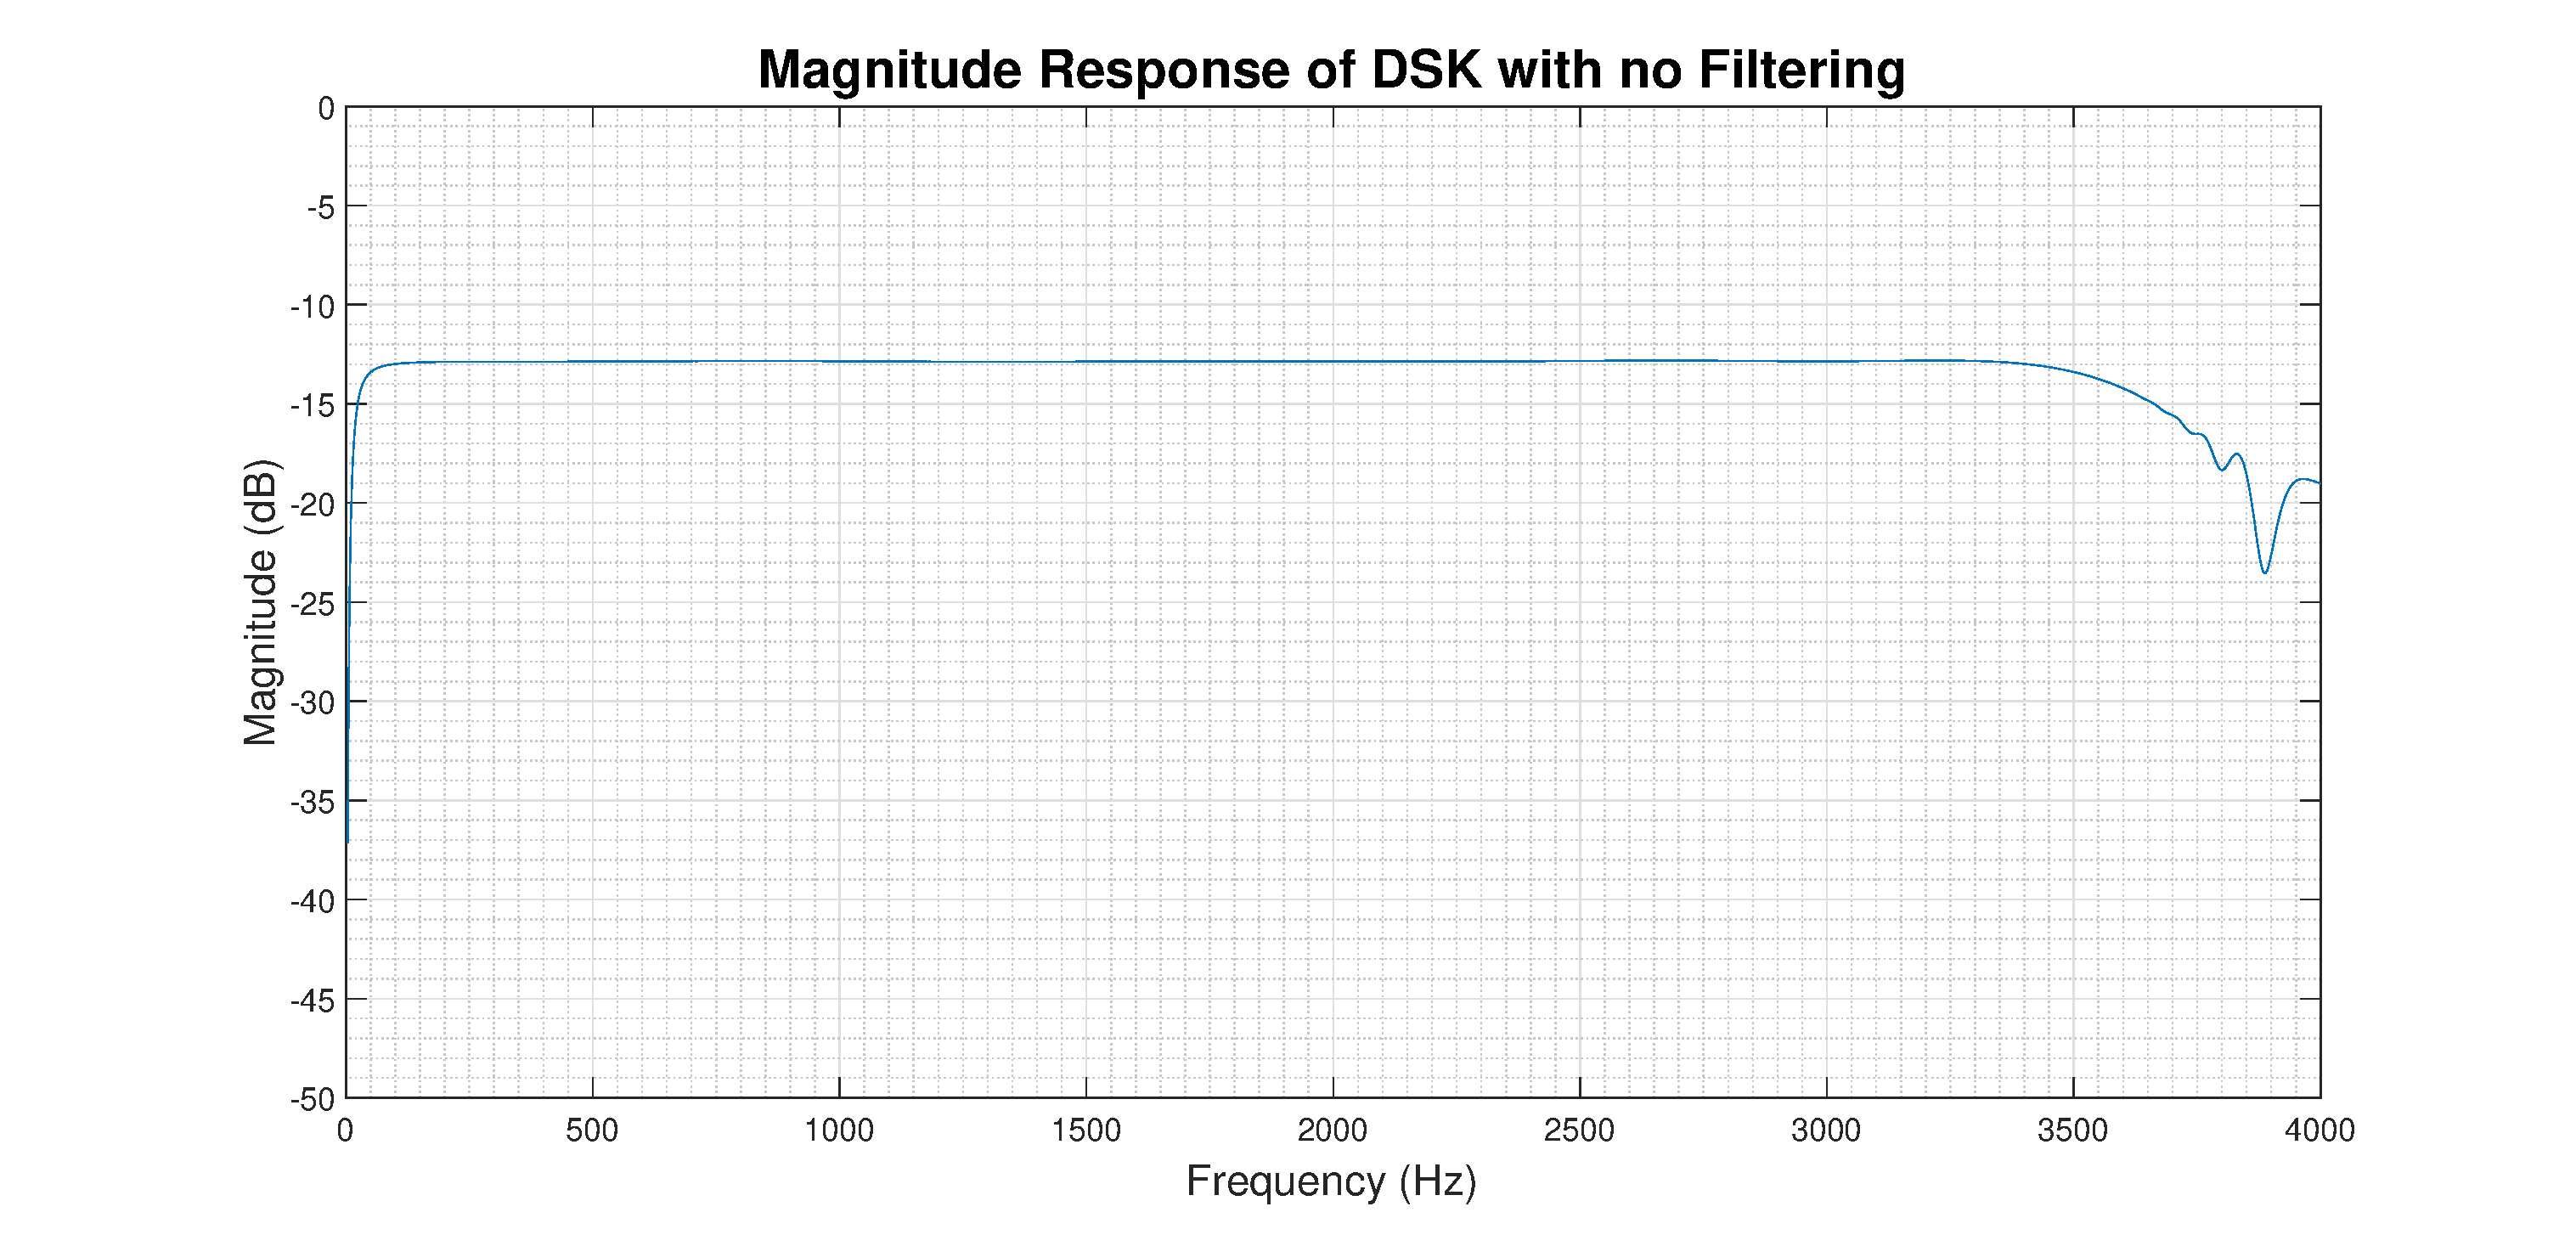
\includegraphics[width=0.49\textwidth]{dsk_mag_no_filter}
    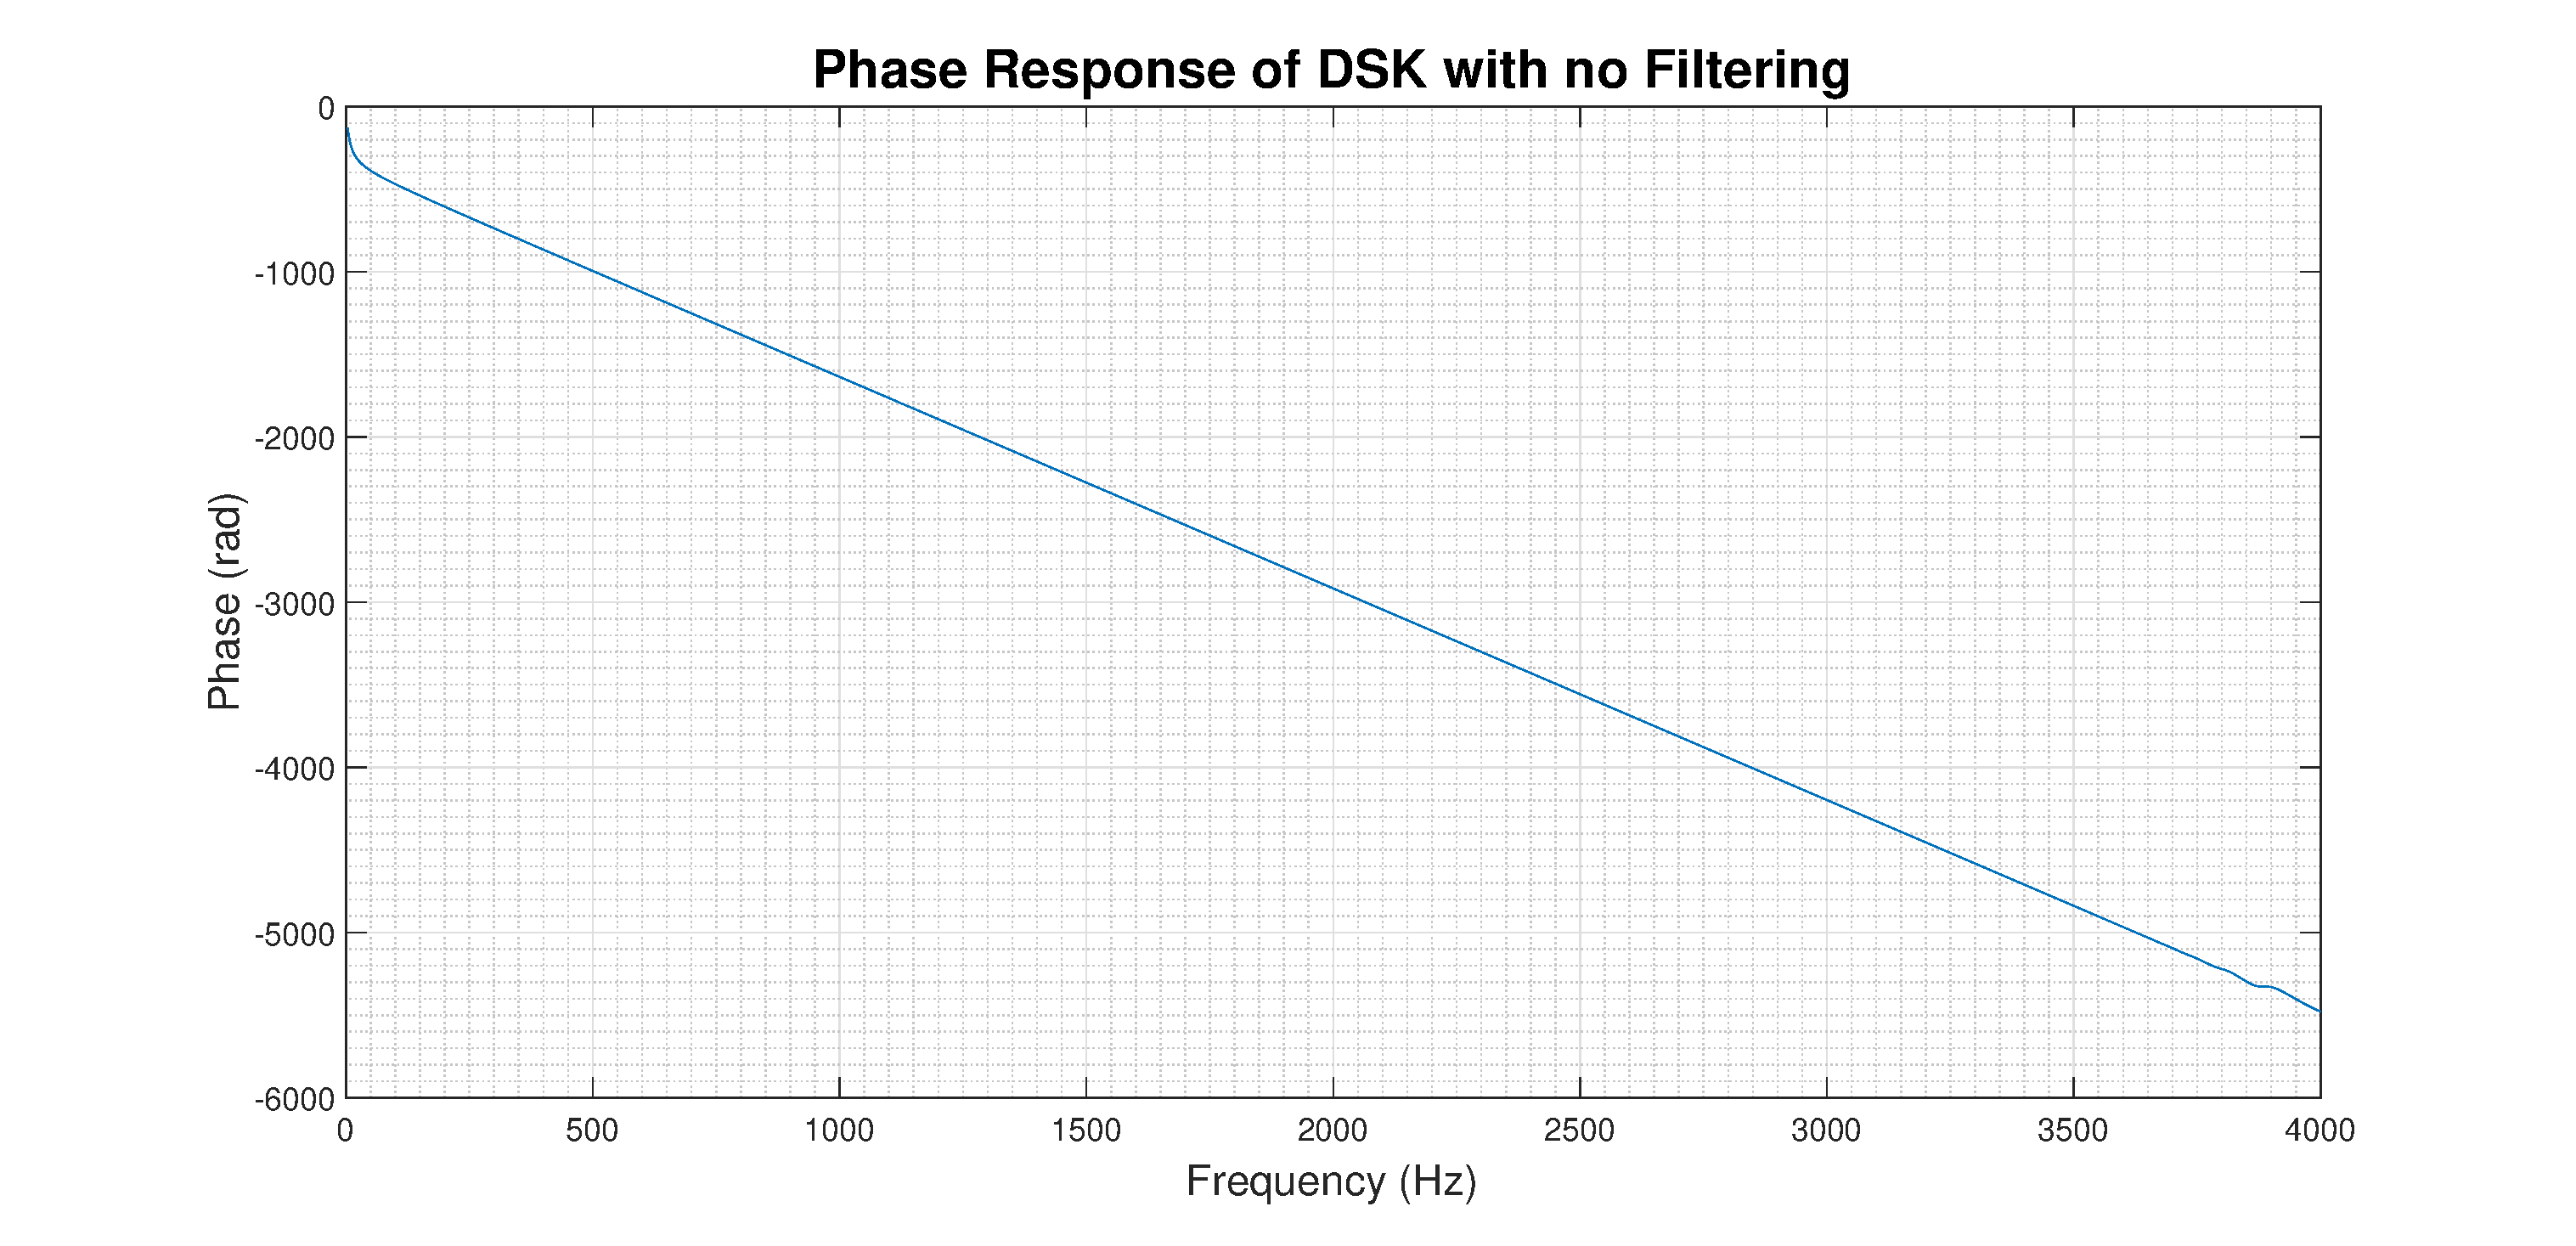
\includegraphics[width=0.49\textwidth]{dsk_phase_no_filter}
    \caption{Frequency response of $TMS320C6713 \ DSK$ board without any filter}
    \label{fig:dsk_response}
\end{figure}

\textbf{Pass band gain of $-13dB$ corresponds to a gain of approximately $\nicefrac{1}{4}$. This is exactly as expected.} The $AIC23$ audio codec is connected to a potential divider with gain $0.5$ externally. In addition, there is a potential divider built into the line inputs with of gain of $0.5$ as well. \textbf{Cascaded, these potential dividers produce a gain of $\nicefrac{1}{4}$.}\\ \\
Next, figure \ref{fig:old_filter} shows the frequency response of the filter designed in section \ref{sec:mat_design}. Note that the magnitude response in the pass band is centred about $-13dB$. This is discrepancy comes about because of the inherent frequency response of the $DSK$ board as discussed above. 

\begin{figure}[H]
    \centering
    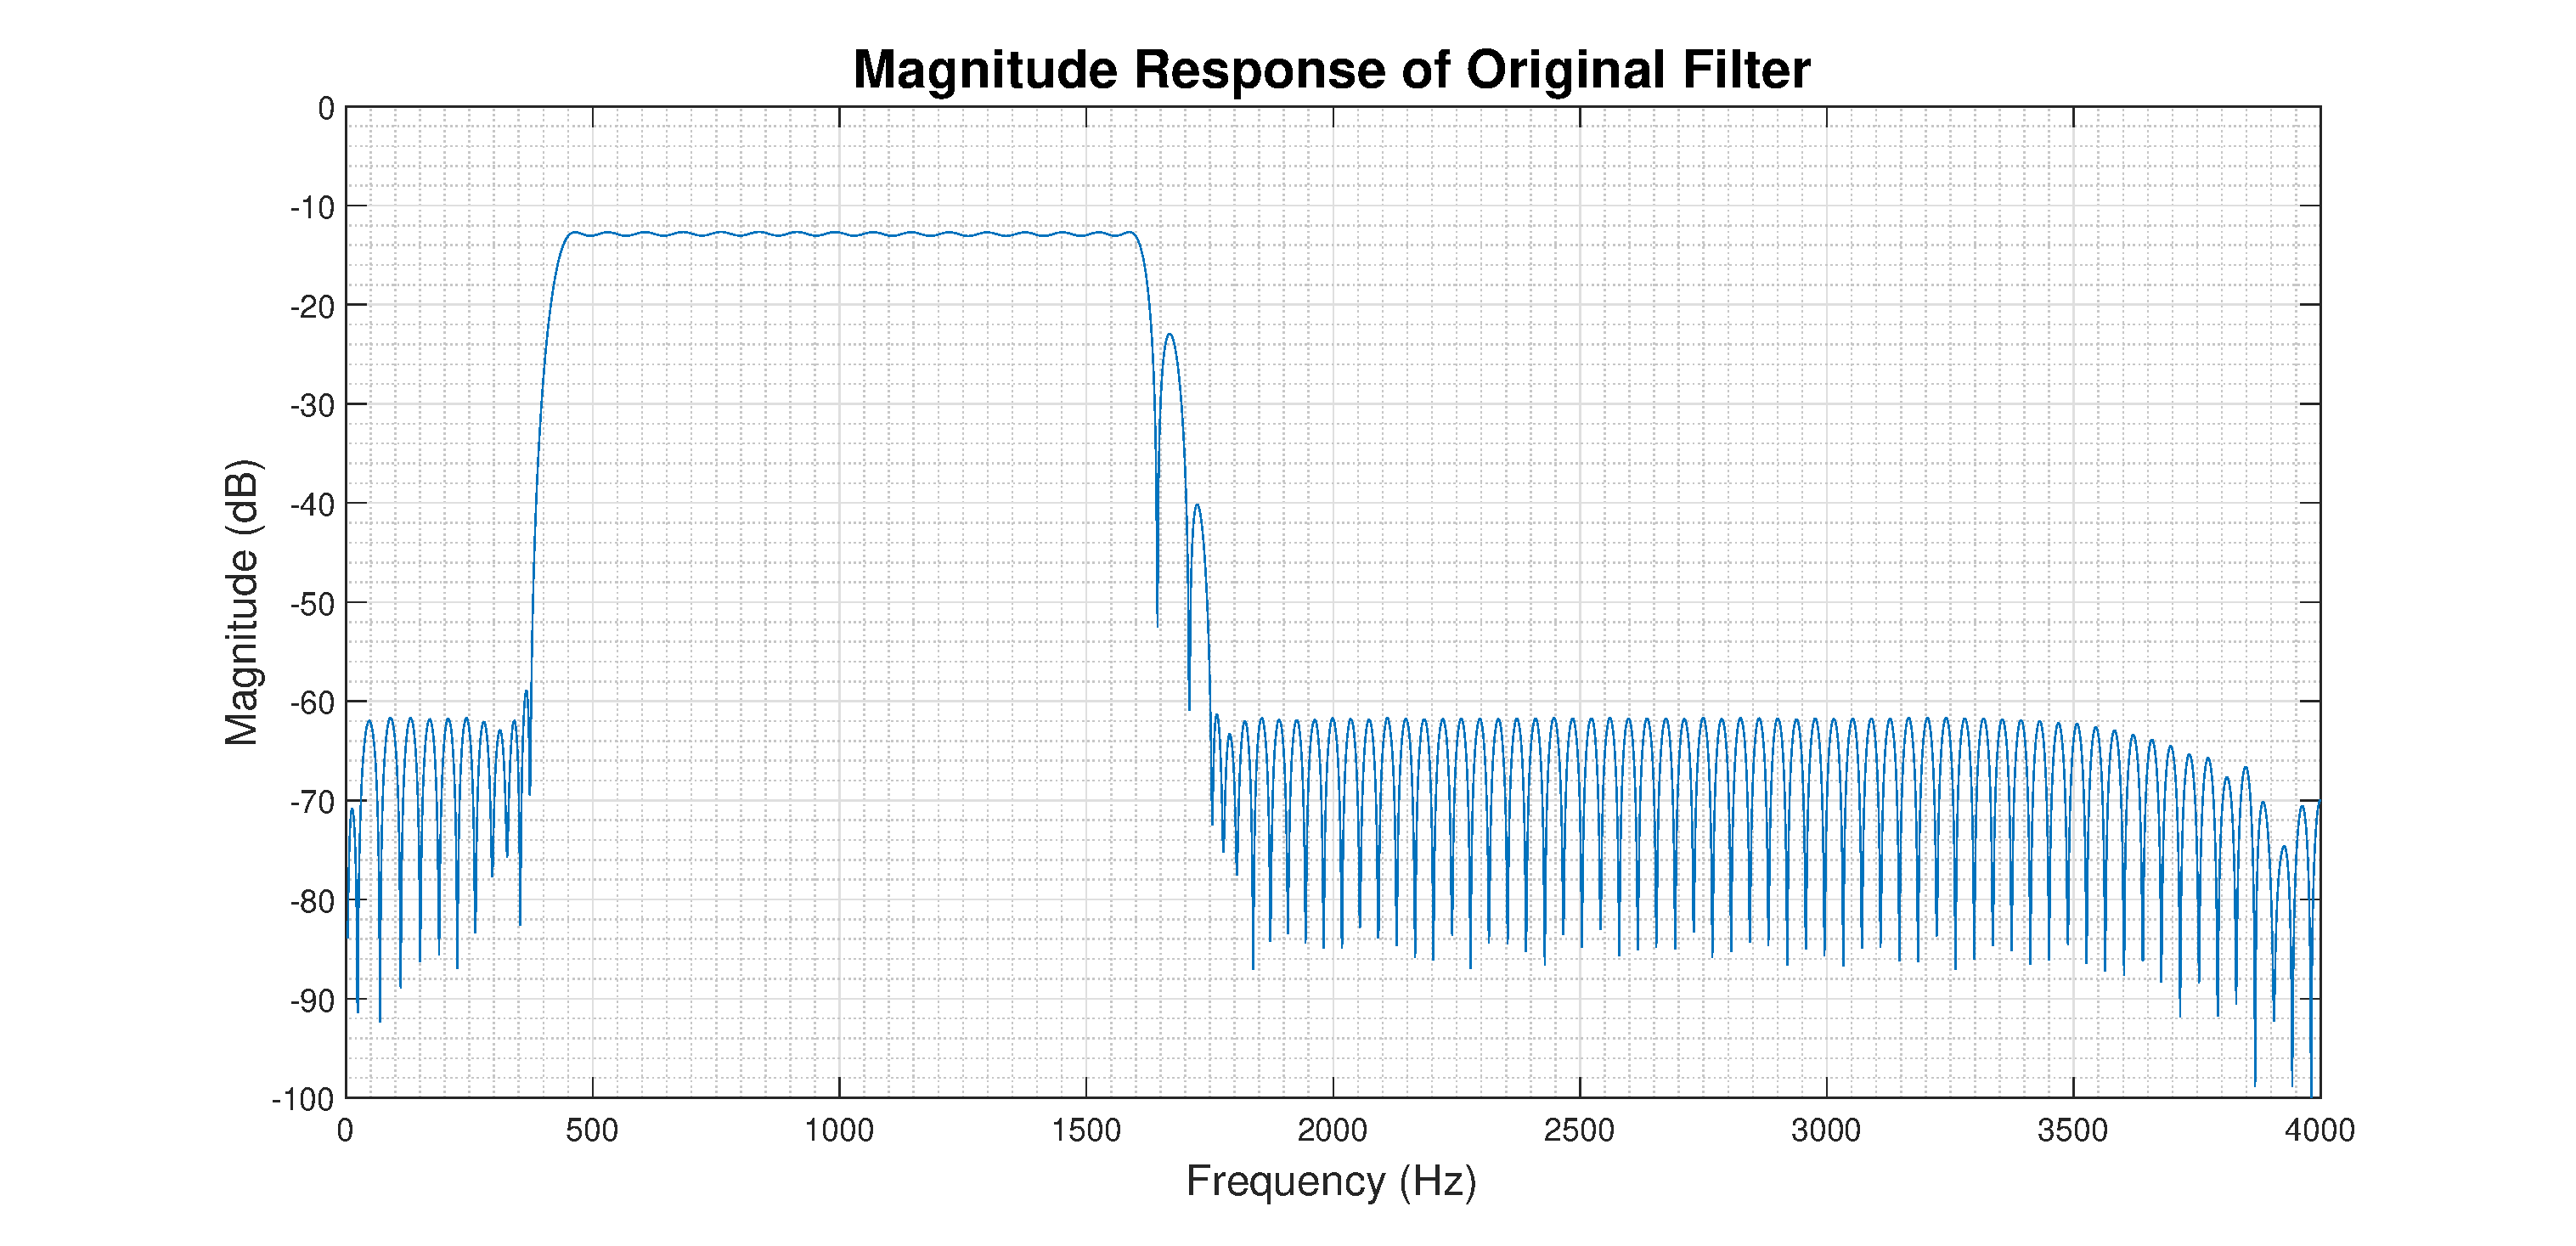
\includegraphics[width=0.49\textwidth]{dsk_mag_original_filter}
    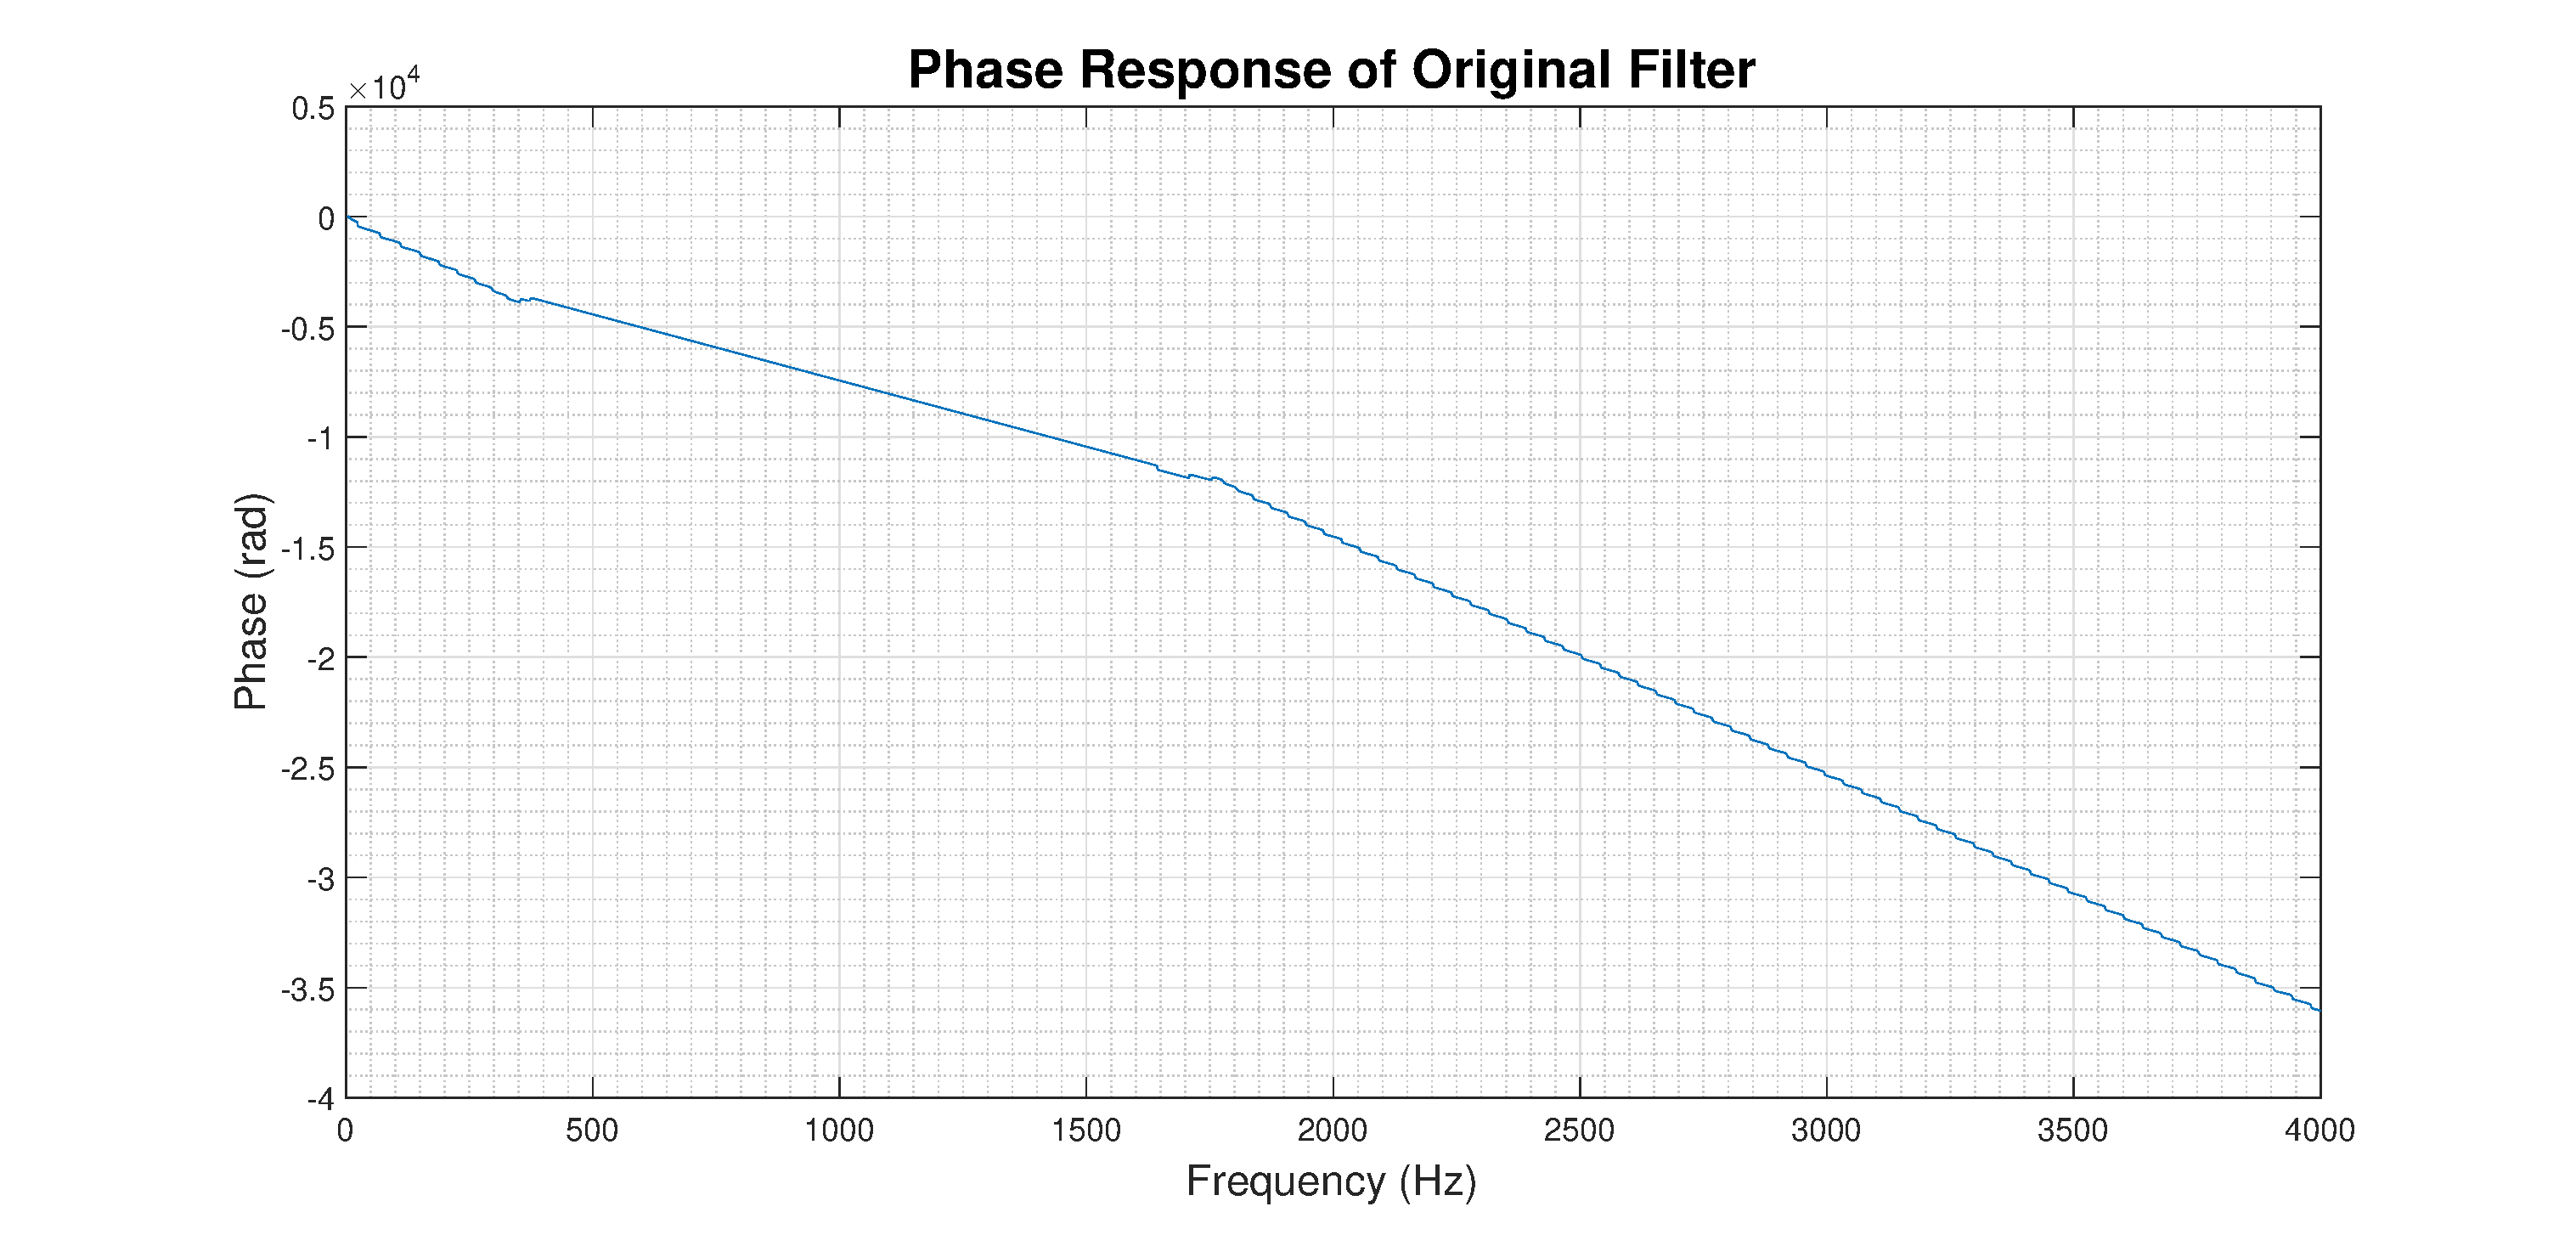
\includegraphics[width=0.49\textwidth]{dsk_phase_original_filter}
    \caption{Frequency response of the filter designed in section \ref{fig:mat_design}}
    \label{fig:old_filter}
\end{figure}

Finally, figure \ref{fig:old_filter_subtracted} shows the frequency response once the offset introduced by the $DSK$ board is taken into account.

\begin{figure}[H]
    \centering
    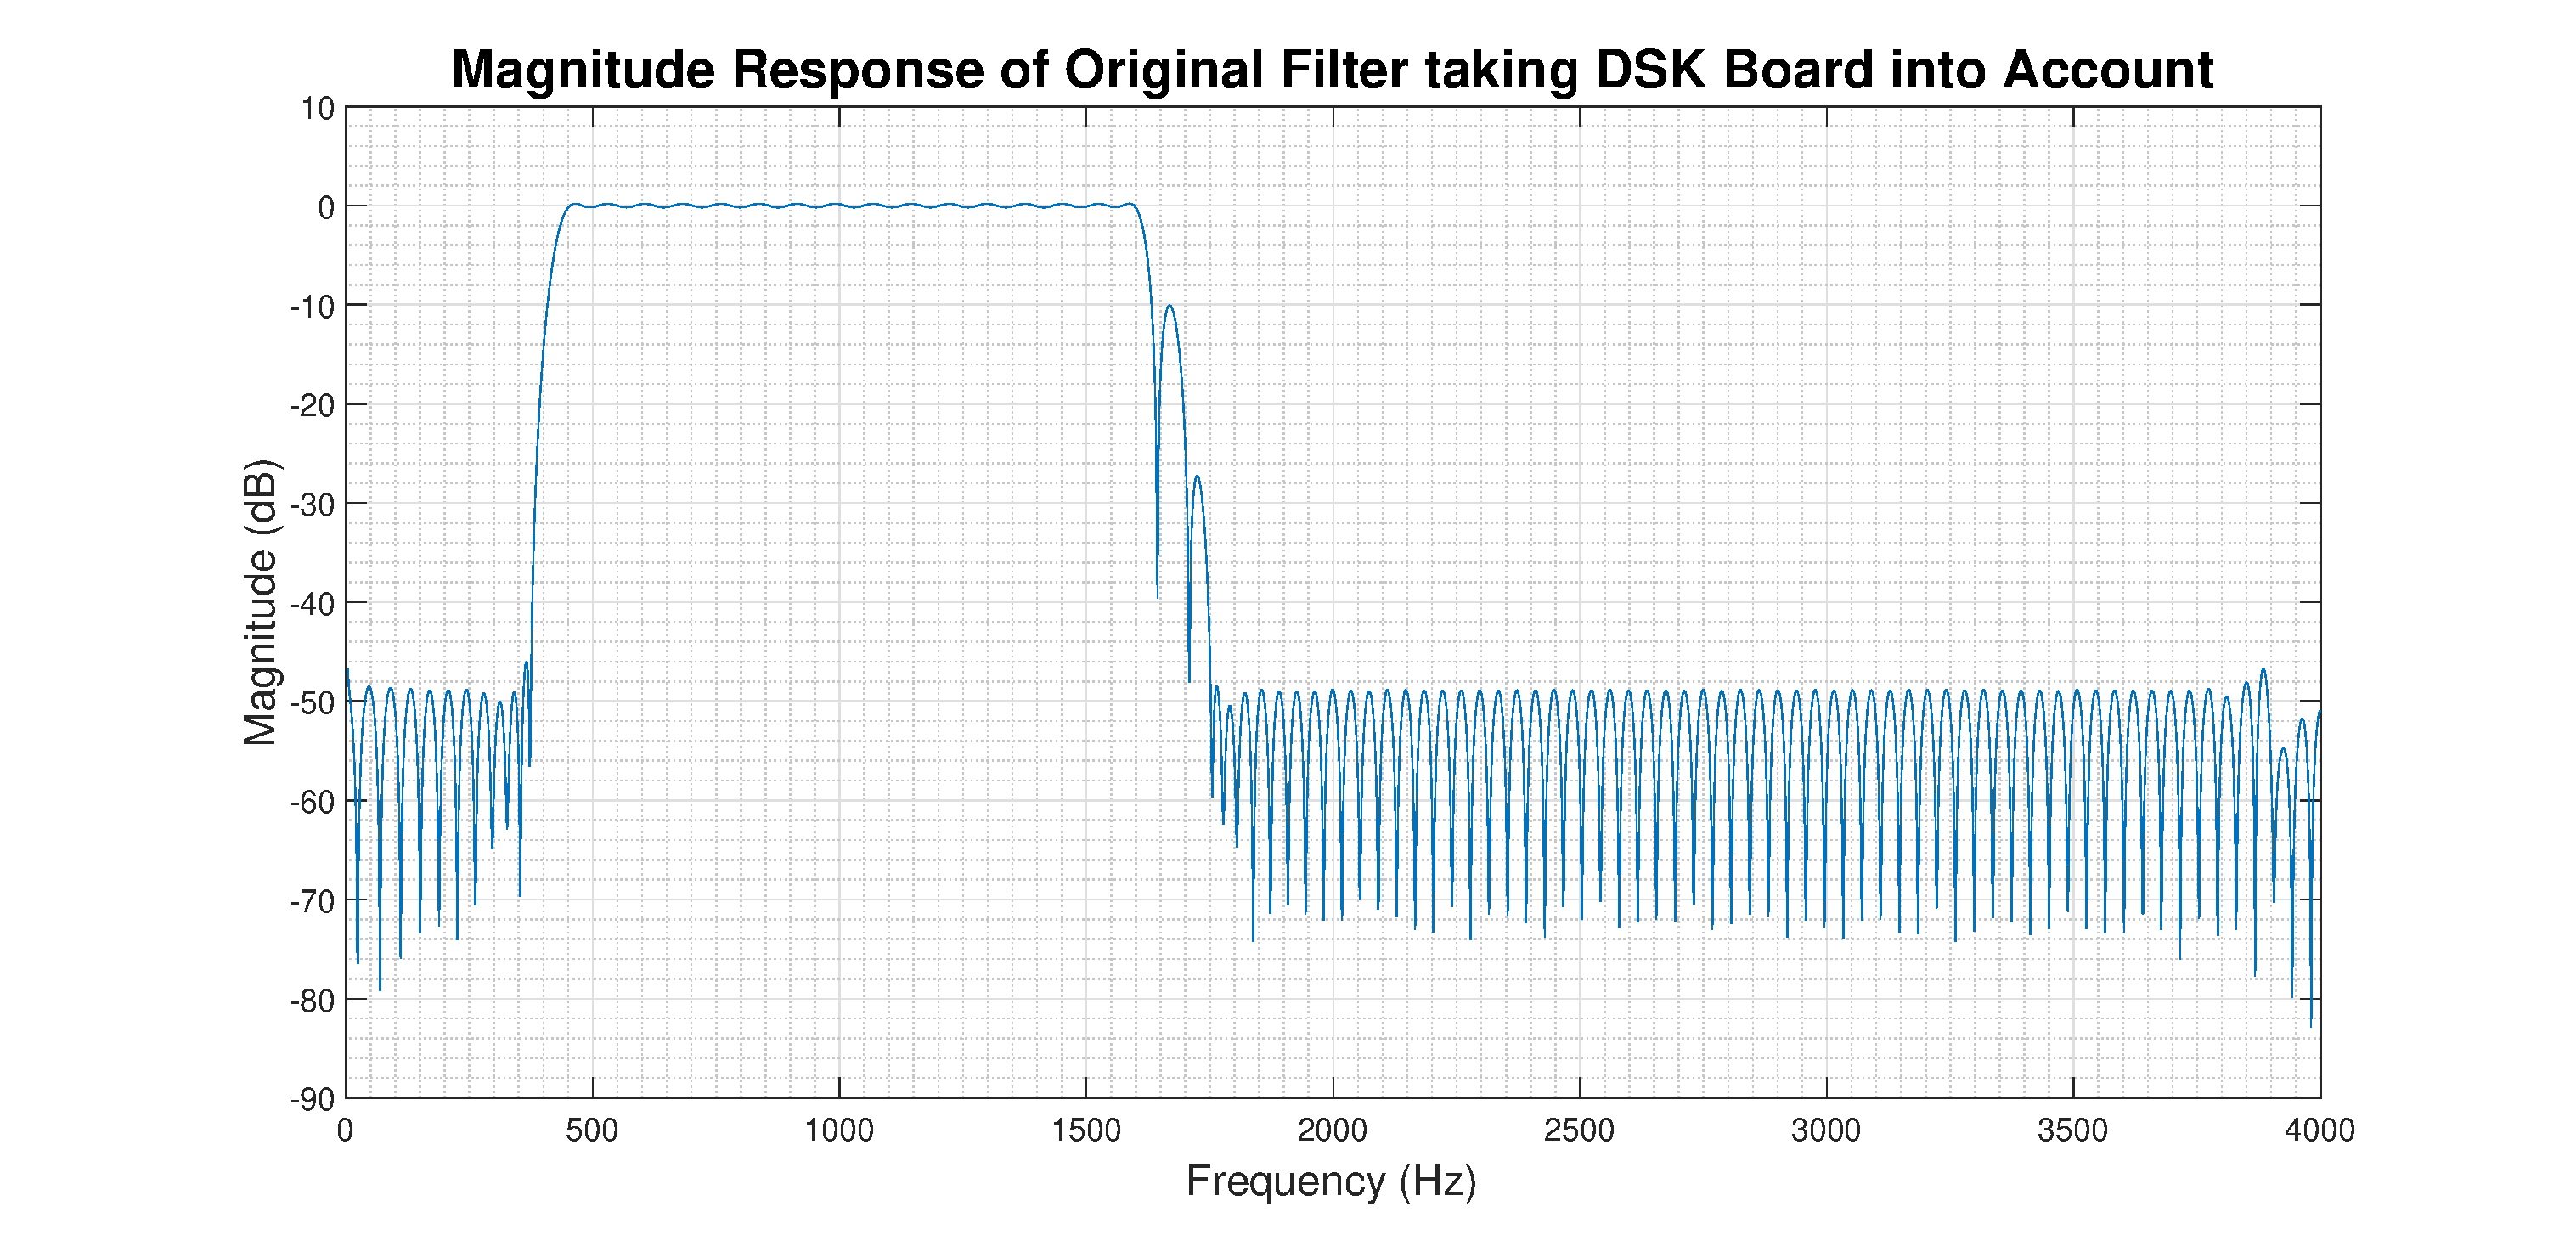
\includegraphics[width=0.49\textwidth]{dsk_mag_original_filter_after_subtracting}
    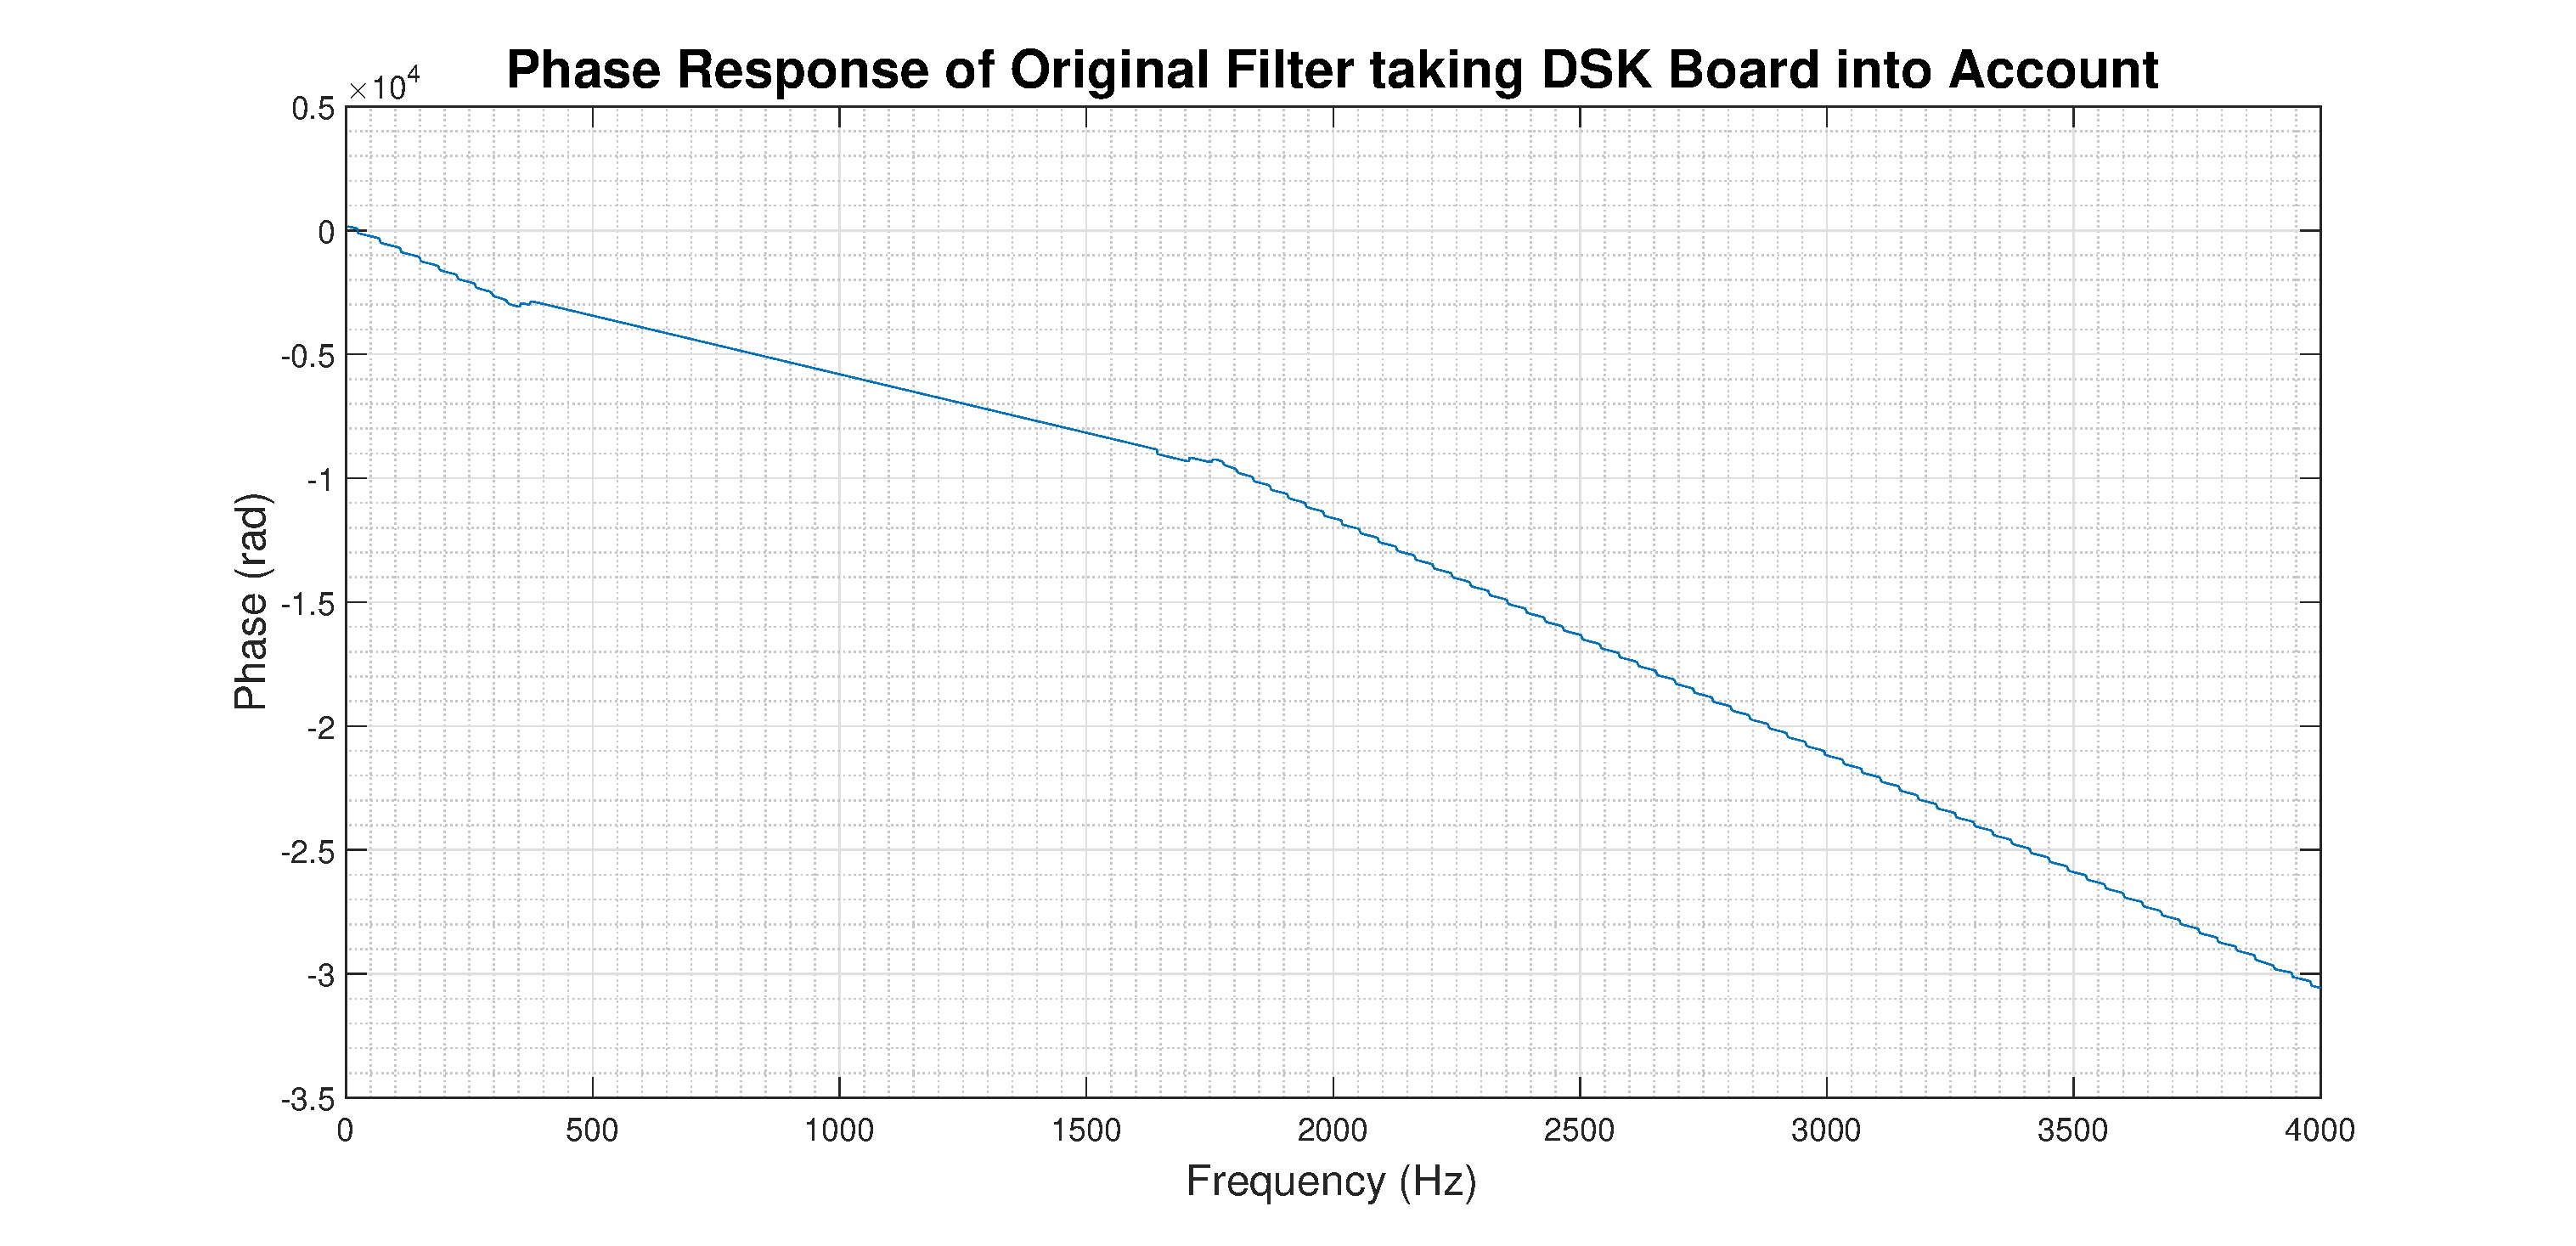
\includegraphics[width=0.49\textwidth]{dsk_phase_original_filter_after_subtracting}
    \caption{Frequency response of filter taking  $TMS320C6713 \ DSK$ board's inherent response into account}
    \label{fig:old_filter_subtracted}
\end{figure}

\newpage
\textbf{The filter designed in section \ref{sec:mat_design} meets all of the specifications on MATLAB, however when implemented on the $TMS320C6713 \ DSK$ board, it fails to satisfy the stop band attenuation\footnote{The phase response of the filter designed in section \ref{sec:mat_design} is not discussed in detail. The filter does not meet satisfy the specifications set out in laboratory 4 and thus a new filter is designed in the next section. Phase response of the new filter is presented.}. Figure \ref{fig:old_failed} shows that the stop band attenuation surpasses the limit of $-48dB$.}

\begin{figure}[H]
    \centering
    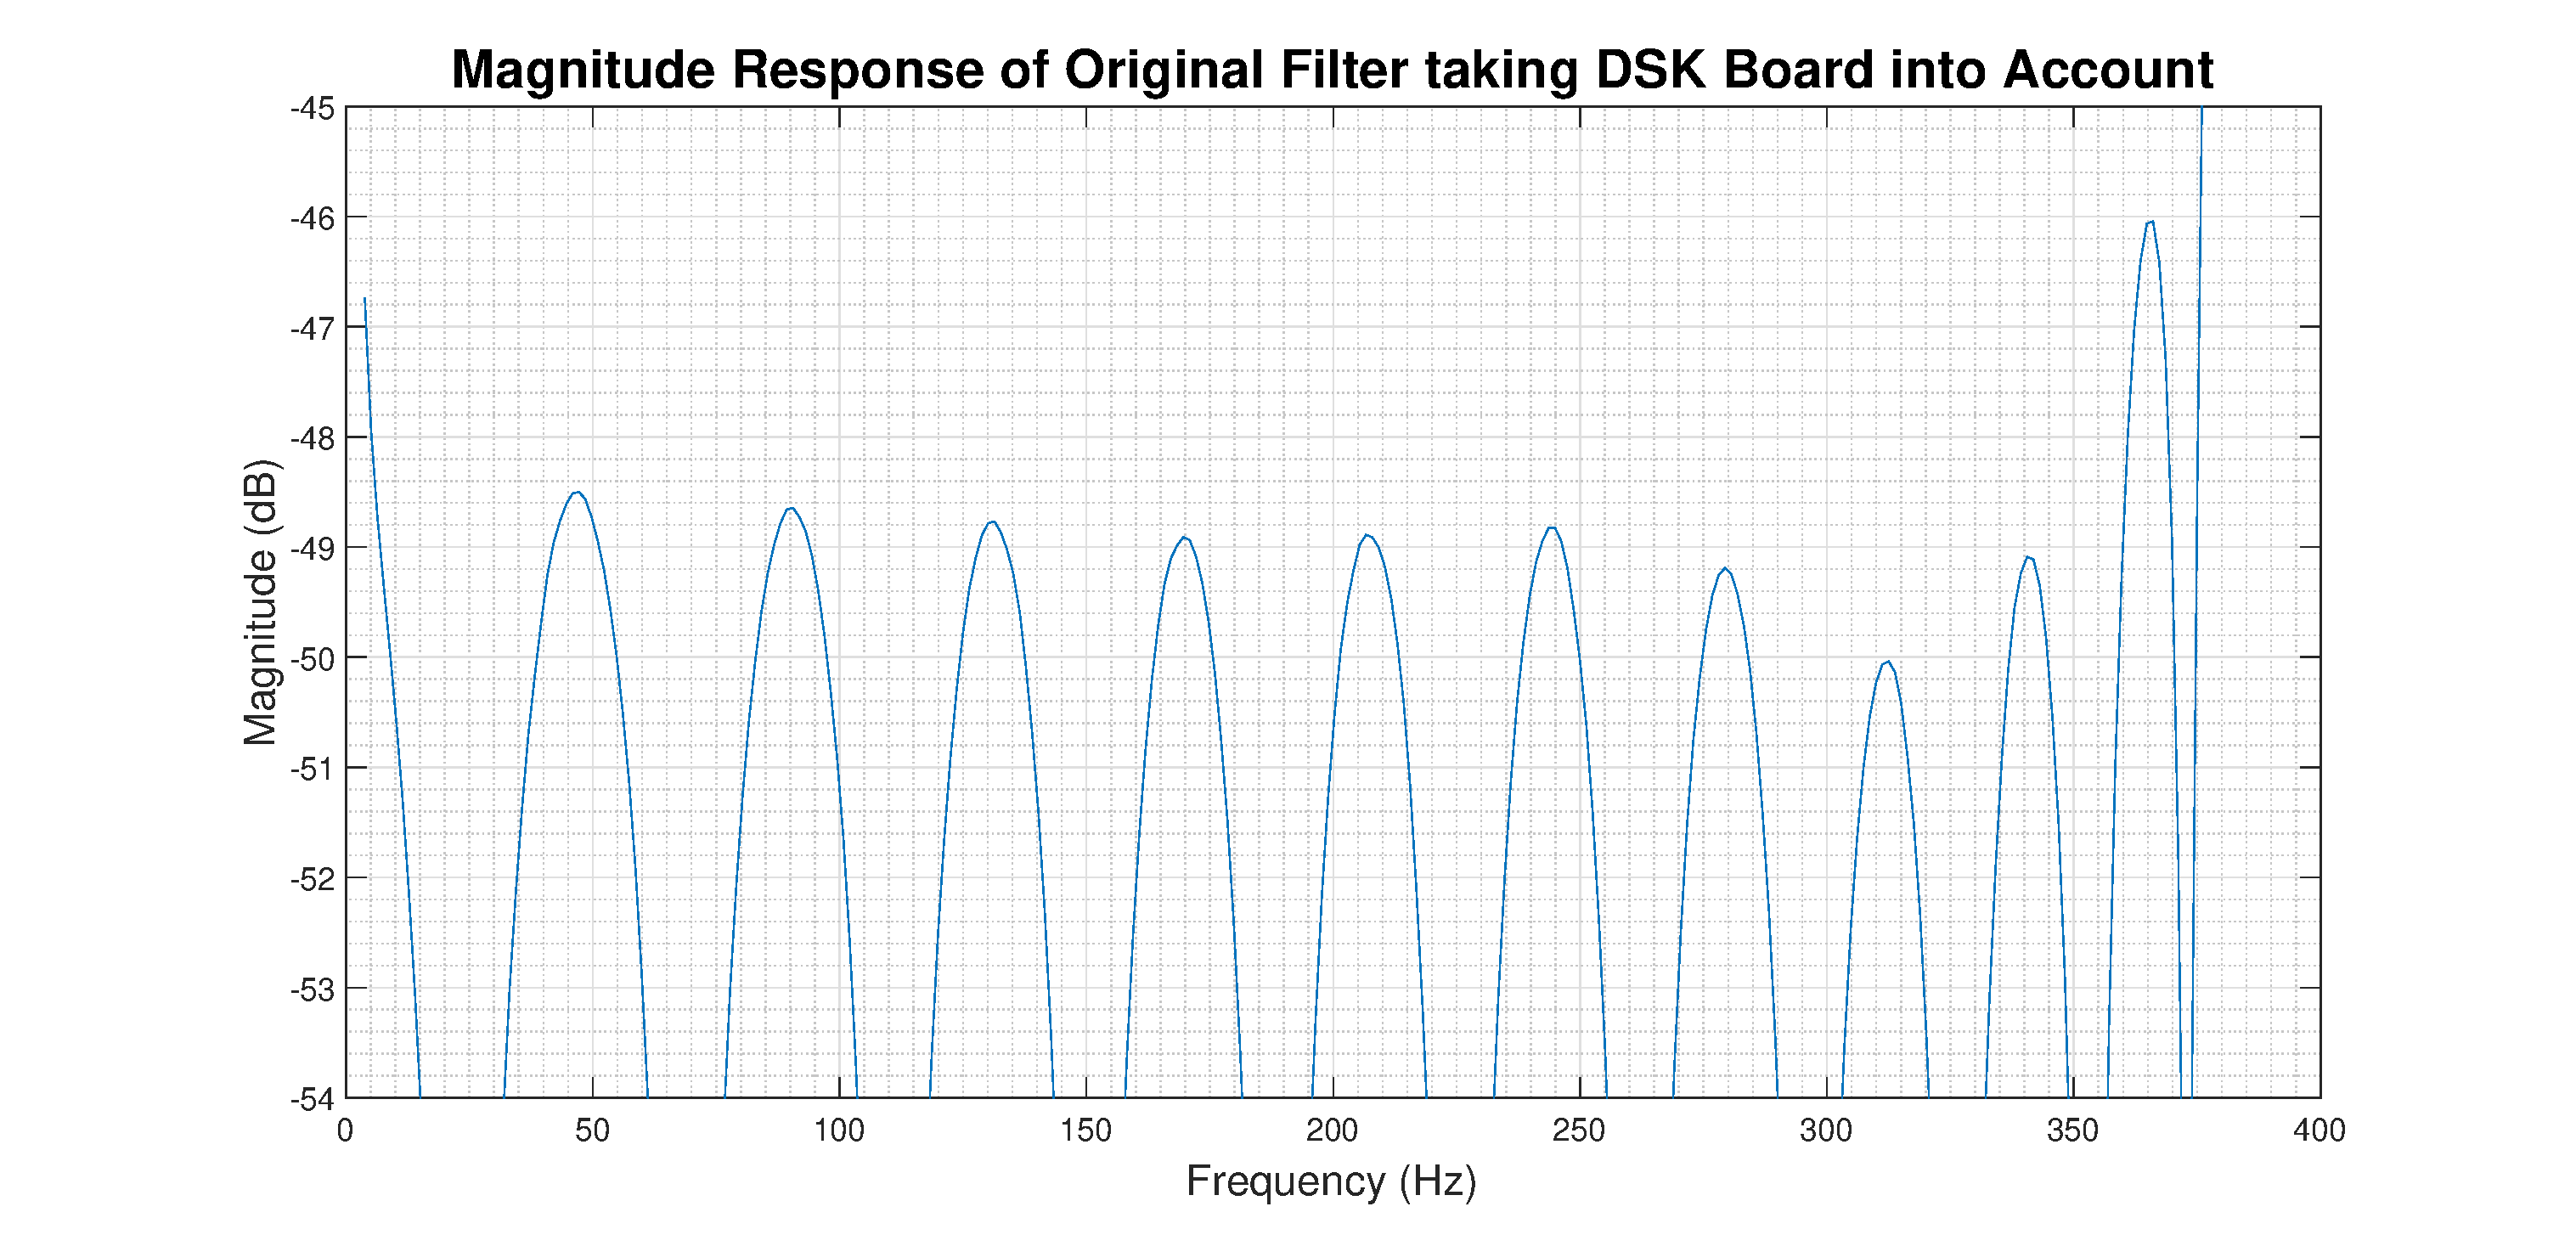
\includegraphics[width=0.65\textwidth]{dsk_mag_original_filter_after_subtracting_artefact}
    \caption{Filter does not meet specified stop band attenuation}
    \label{fig:old_failed}
\end{figure}

\subsection{Improved Filter Design}
To ensure that the filter meets all of the specifications, a new filter is designed on MATLAB. Listing \ref{lst:new_matlab} shows the MATLAB code used to generate the new filter. \textbf{The stop band attenuation and pass band ripple are over specified to $-52dB$ and $0.36dB$ respectively.} In addition, the transition band edges have been tweaked slightly. 

\begin{listing}[H]
\begin{minted}[fontsize=\scriptsize,linenos]{MATLAB}
rp = 0.36;                          % defines the passband ripple
rs = 52;                            % defines the stop band attenuation
F_sampling = 8000;                  % defines the sampling frequency
F_cutoff = [373 450 1600 1700];     % defines the cutoff frequencies
filter_amplitudes = [0 1 0];        % defines ideal gain of each band

% functiuon used to estimate variables need for firpm function
[N, Fo, Ao, W] = firpmord(  F_cutoff,...
                            filter_amplitudes,...
                            [10^(-rs/20) (10^(rp/20)-1)/(10^(rp/20)+1) 10^(-rs/20)],...
                            F_sampling);

                        
coefs = firpm(N+4, Fo, Ao, W);      % order of filter is increased by 4 to meet specifications

[h,w] = freqz(coefs, [1], 2^16);
\end{minted}
\caption{MATLAB code to generate coefficients for an improved FIR filter} 
\label{lst:new_matlab}
\end{listing}

\textbf{The improved filter requires $221$ coefficients instead of $211$ to be implemented.} Figure \ref{fig:new_filer} shows the magnitude response of the new filter. Note that this plot already takes into account the inherent frequency response of the $TMS320C6713 \ DSK$ board. \textbf{The plot also includes the theoretical frequency response and it is clear that the filter performs exactly as expected.}

\begin{figure}[H]
    \centering
    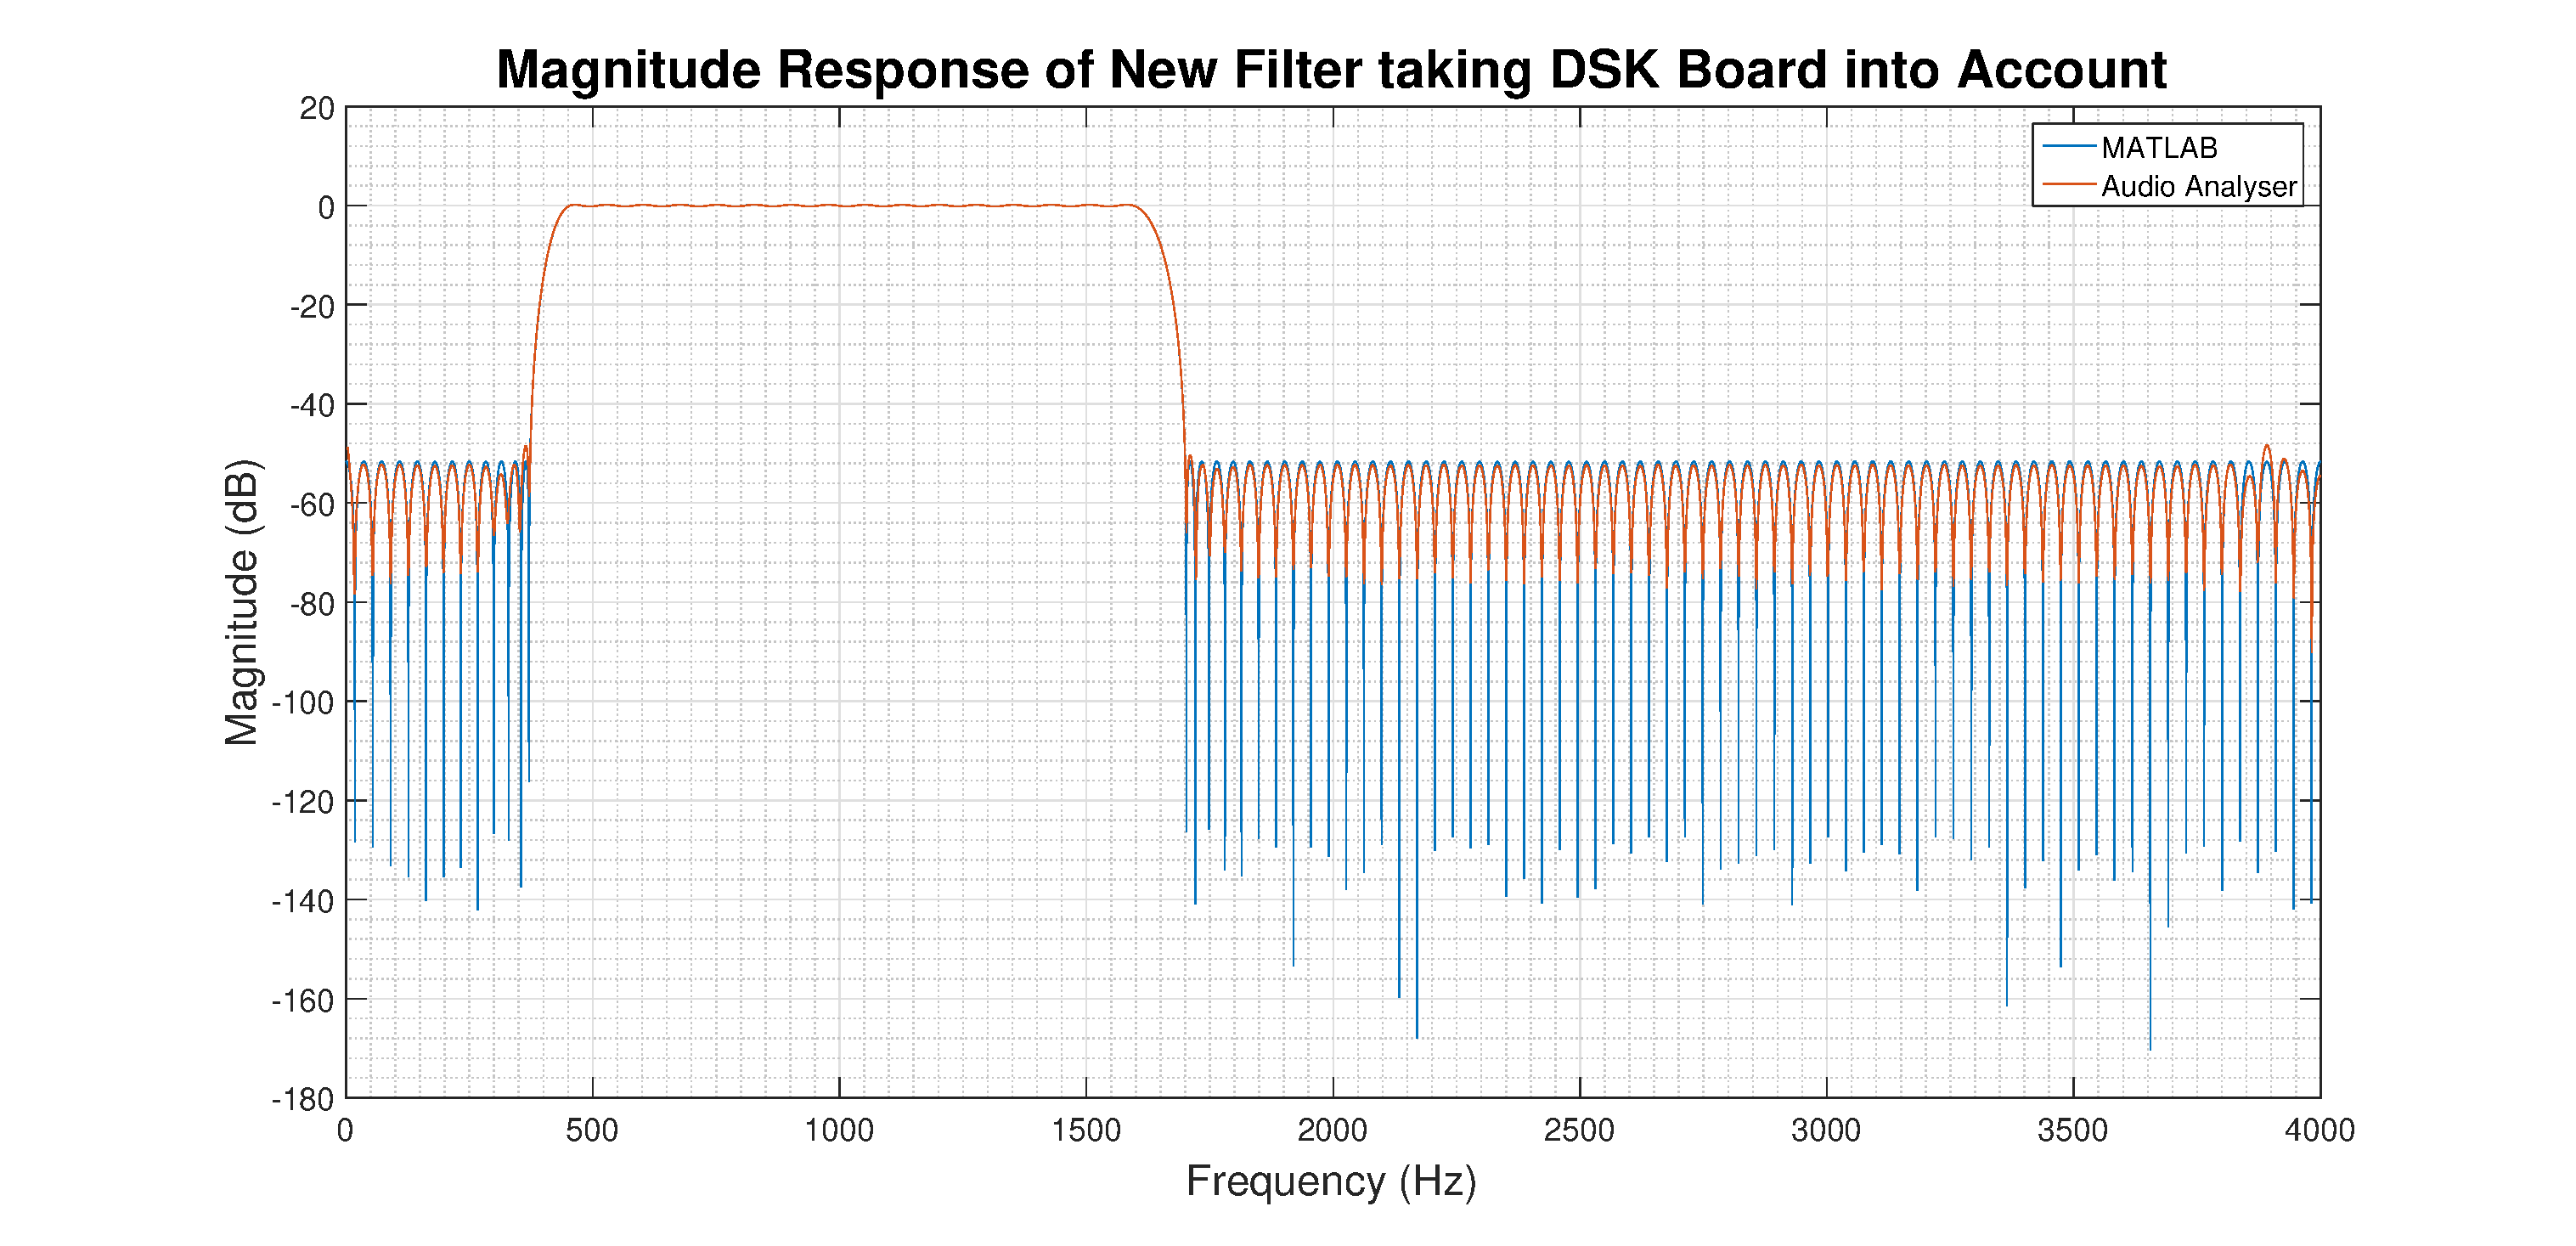
\includegraphics[width=0.55\textwidth]{dsk_mag_new_filter_after_subtracting}
    \caption{Magnitude response of improved filter}
    \label{fig:new_filer}
\end{figure}

Figure \ref{fig:new_filter_zoom} plots the frequency response of filter for specific frequencies. \textbf{The plot confirms that the magnitude spectrum of the improved filter satisfies all the specifications set out in laboratory 4.}

\begin{figure}[H]
    \centering
    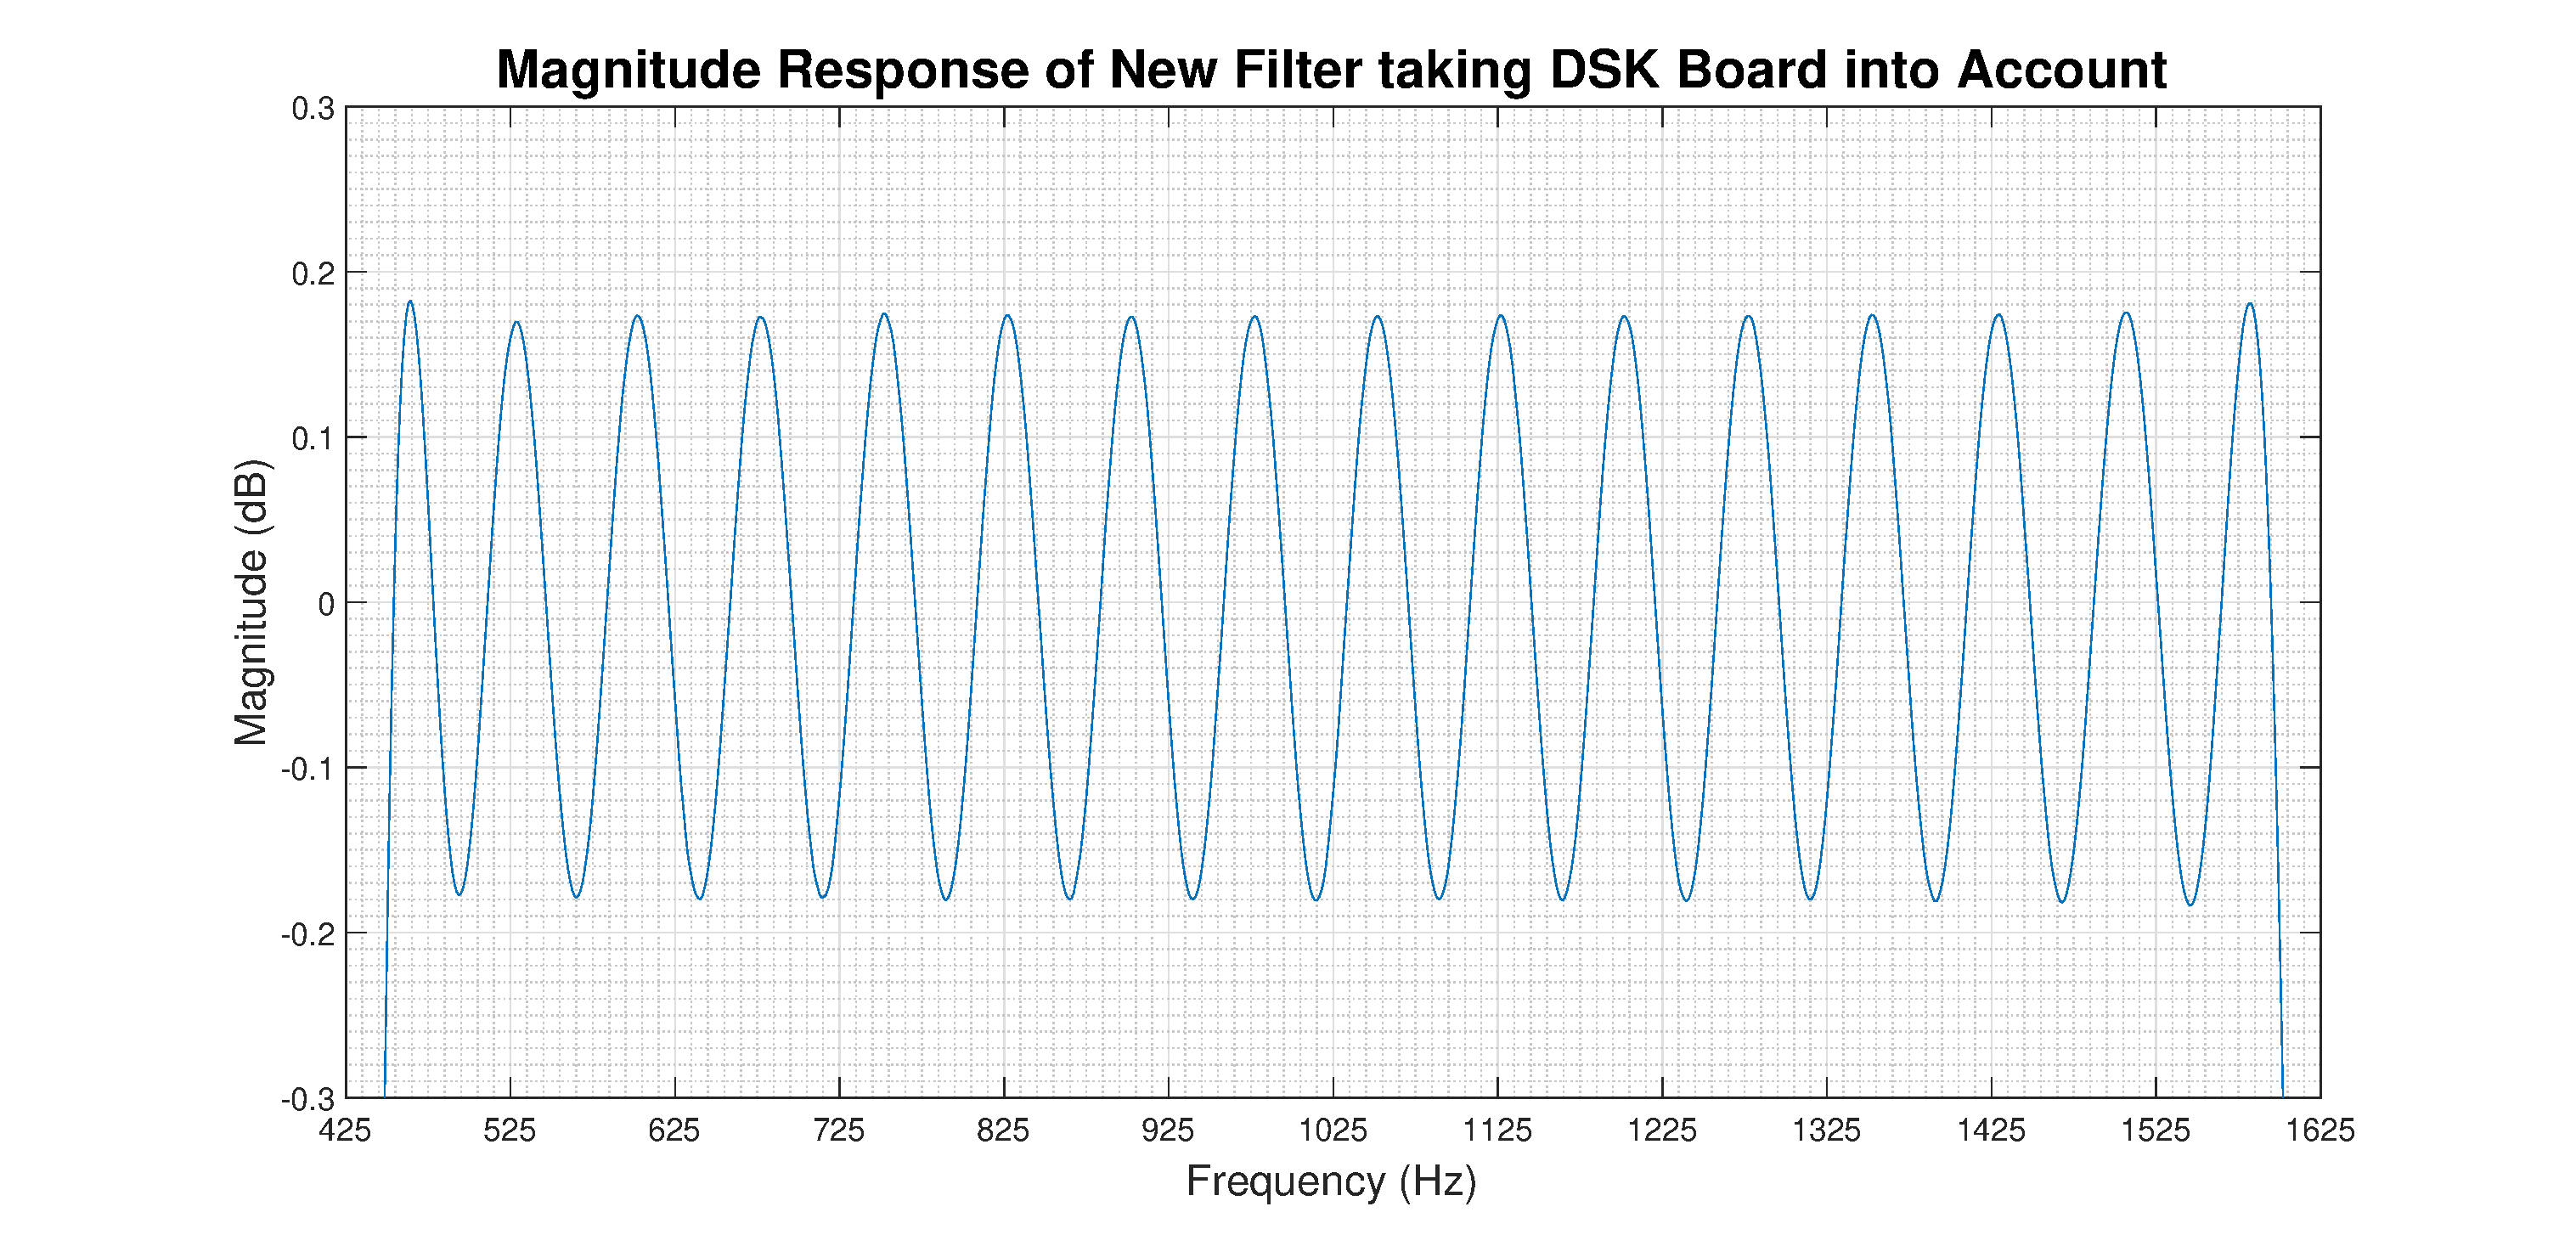
\includegraphics[width=0.8\textwidth]{dsk_mag_new_filter_after_subtracting_passband_zoom}
    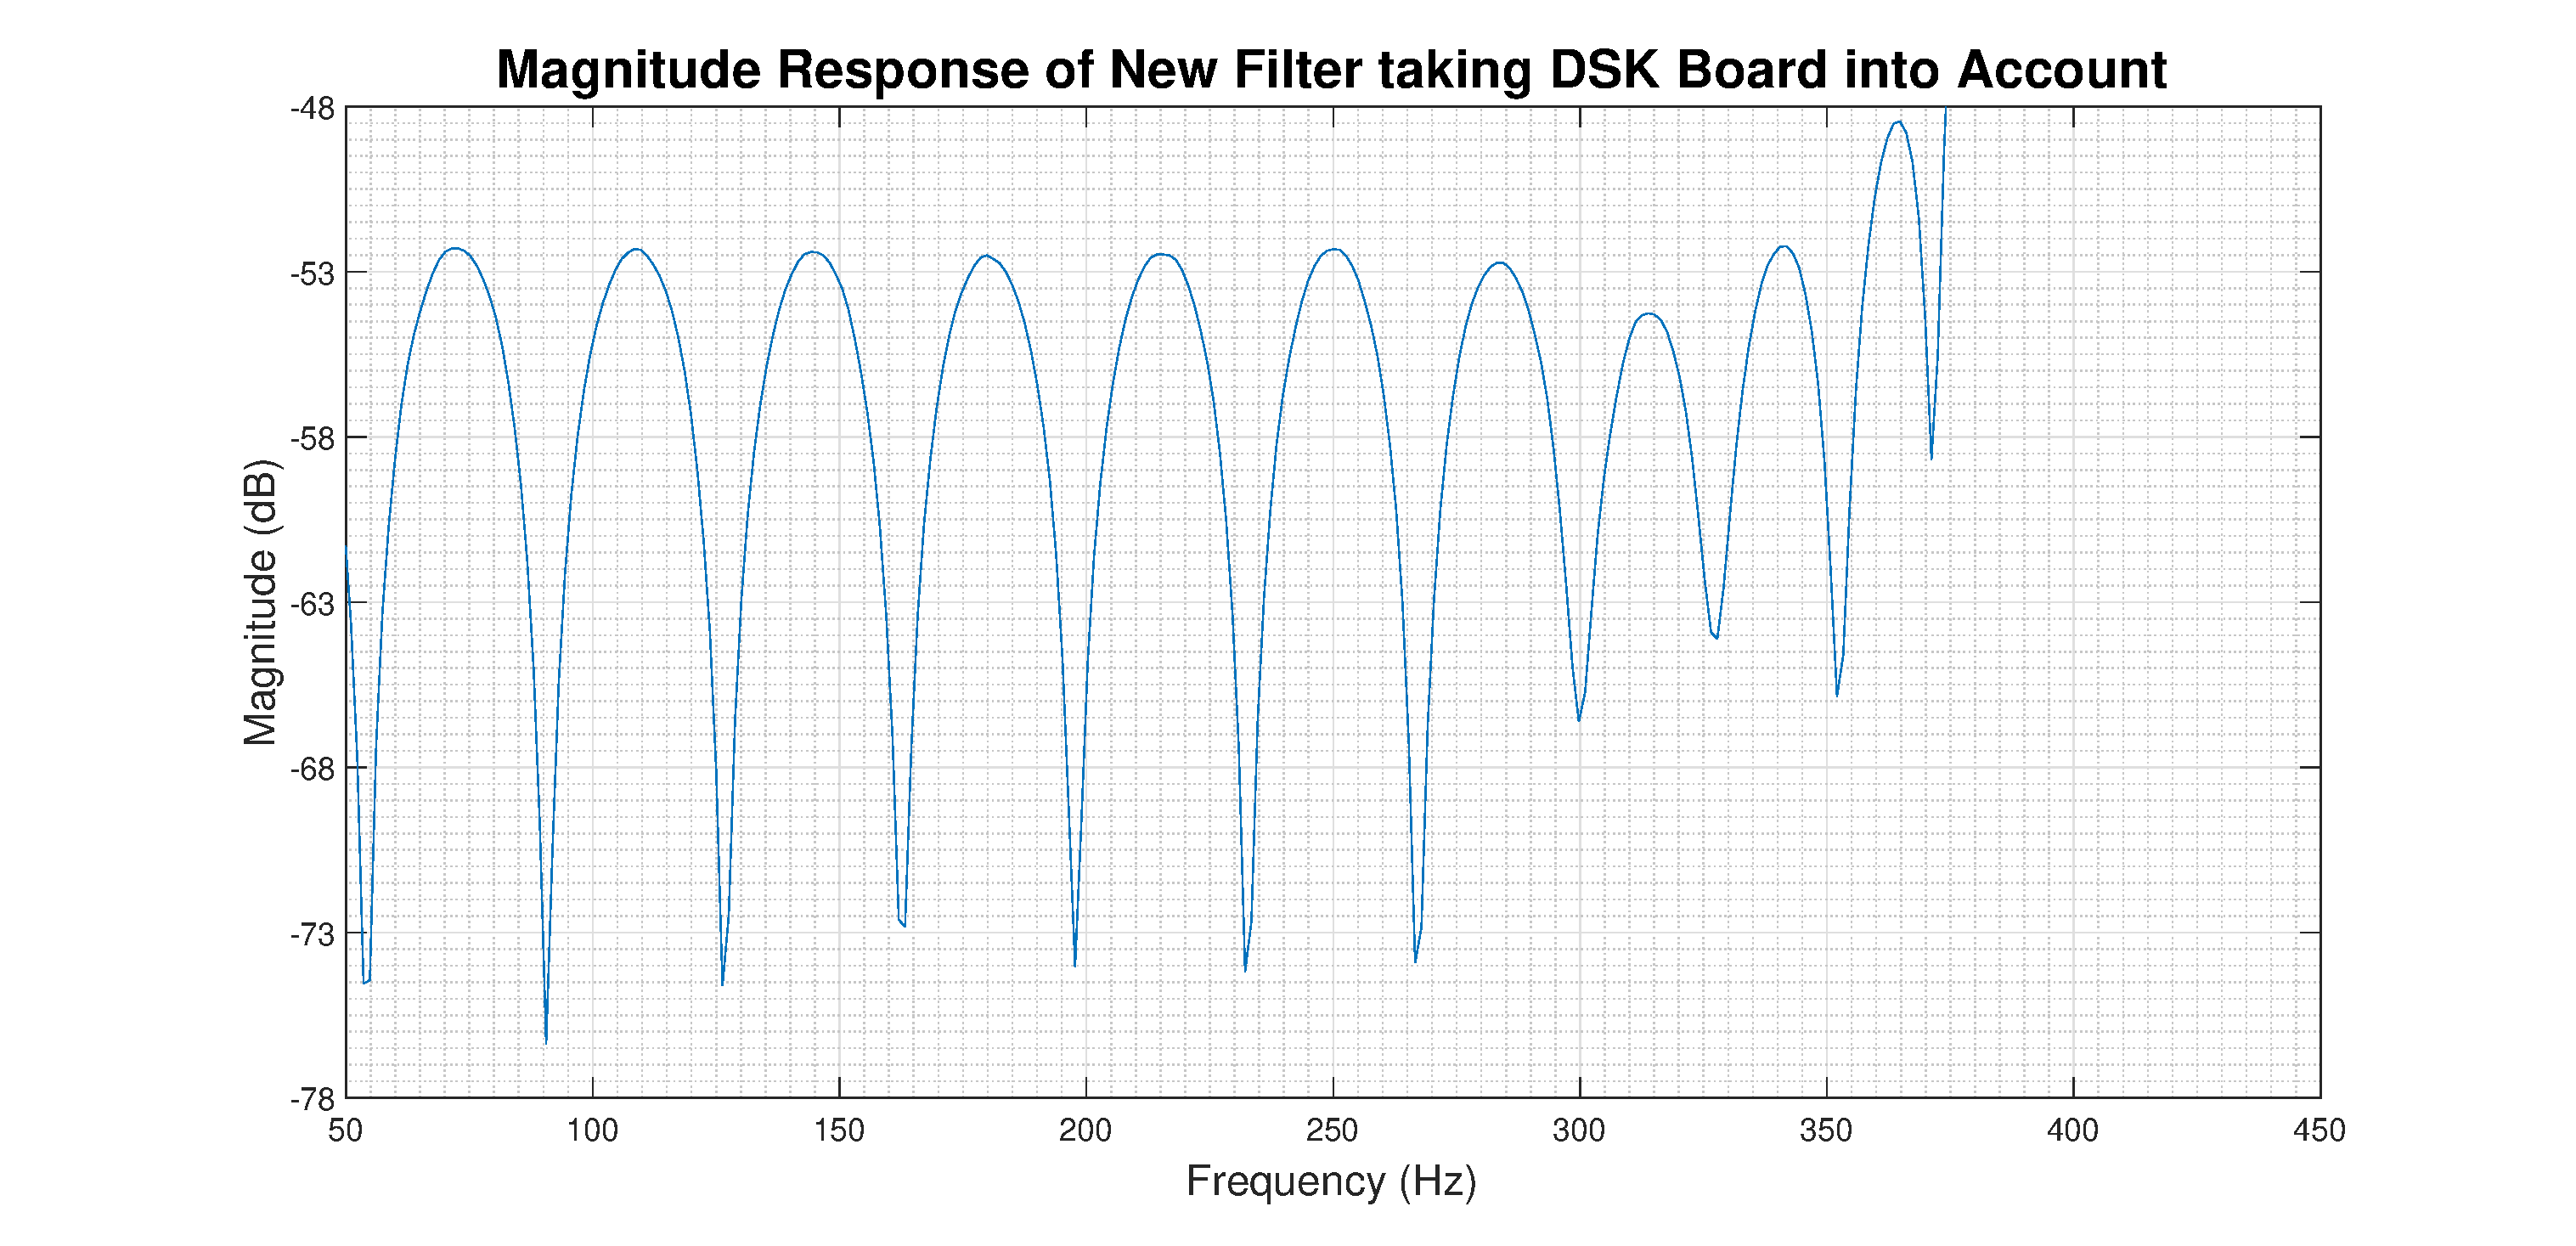
\includegraphics[width=0.8\textwidth]{dsk_mag_new_filter_after_subtracting_stopband_1_zoom}
    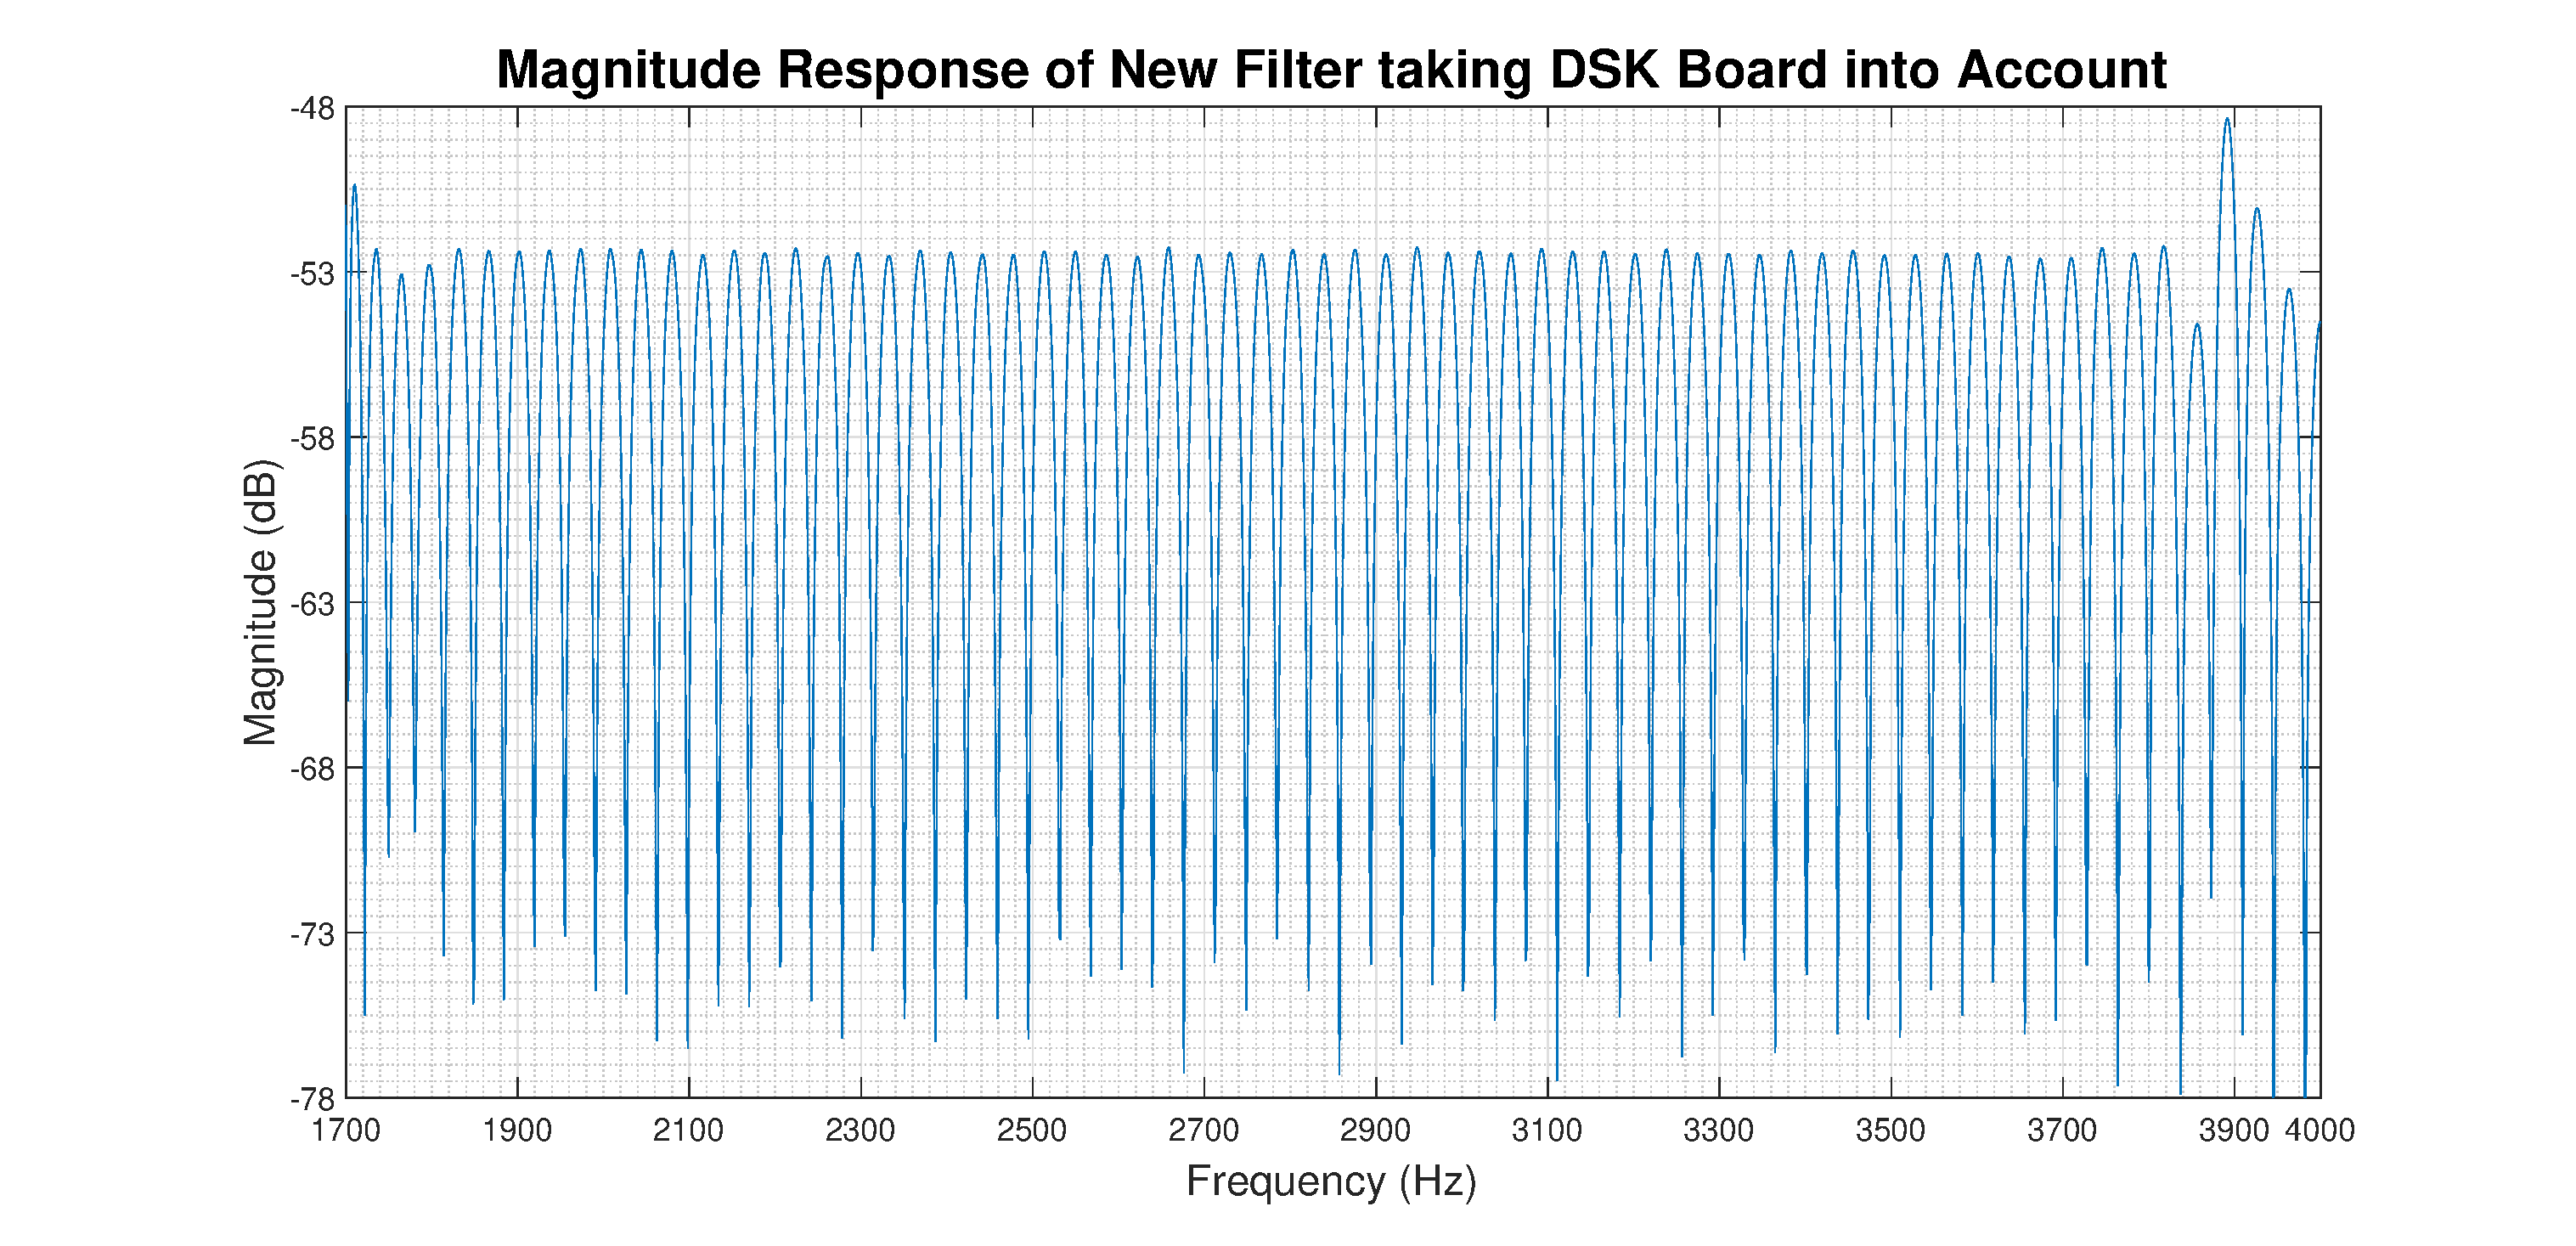
\includegraphics[width=0.8\textwidth]{dsk_mag_new_filter_after_subtracting_stopband_2_zoom}
    \caption{Magnitude response of improved filter}
    \label{fig:new_filter_zoom}
\end{figure}

\newpage
Next, the phase response of the improved filter is studied. Figure \ref{fig:new_filter_phase_for_calc} shows the phase response of the filter and confirms the fact that the phase in indeed linear in the pass band. 

\begin{figure}[H]
    \centering
    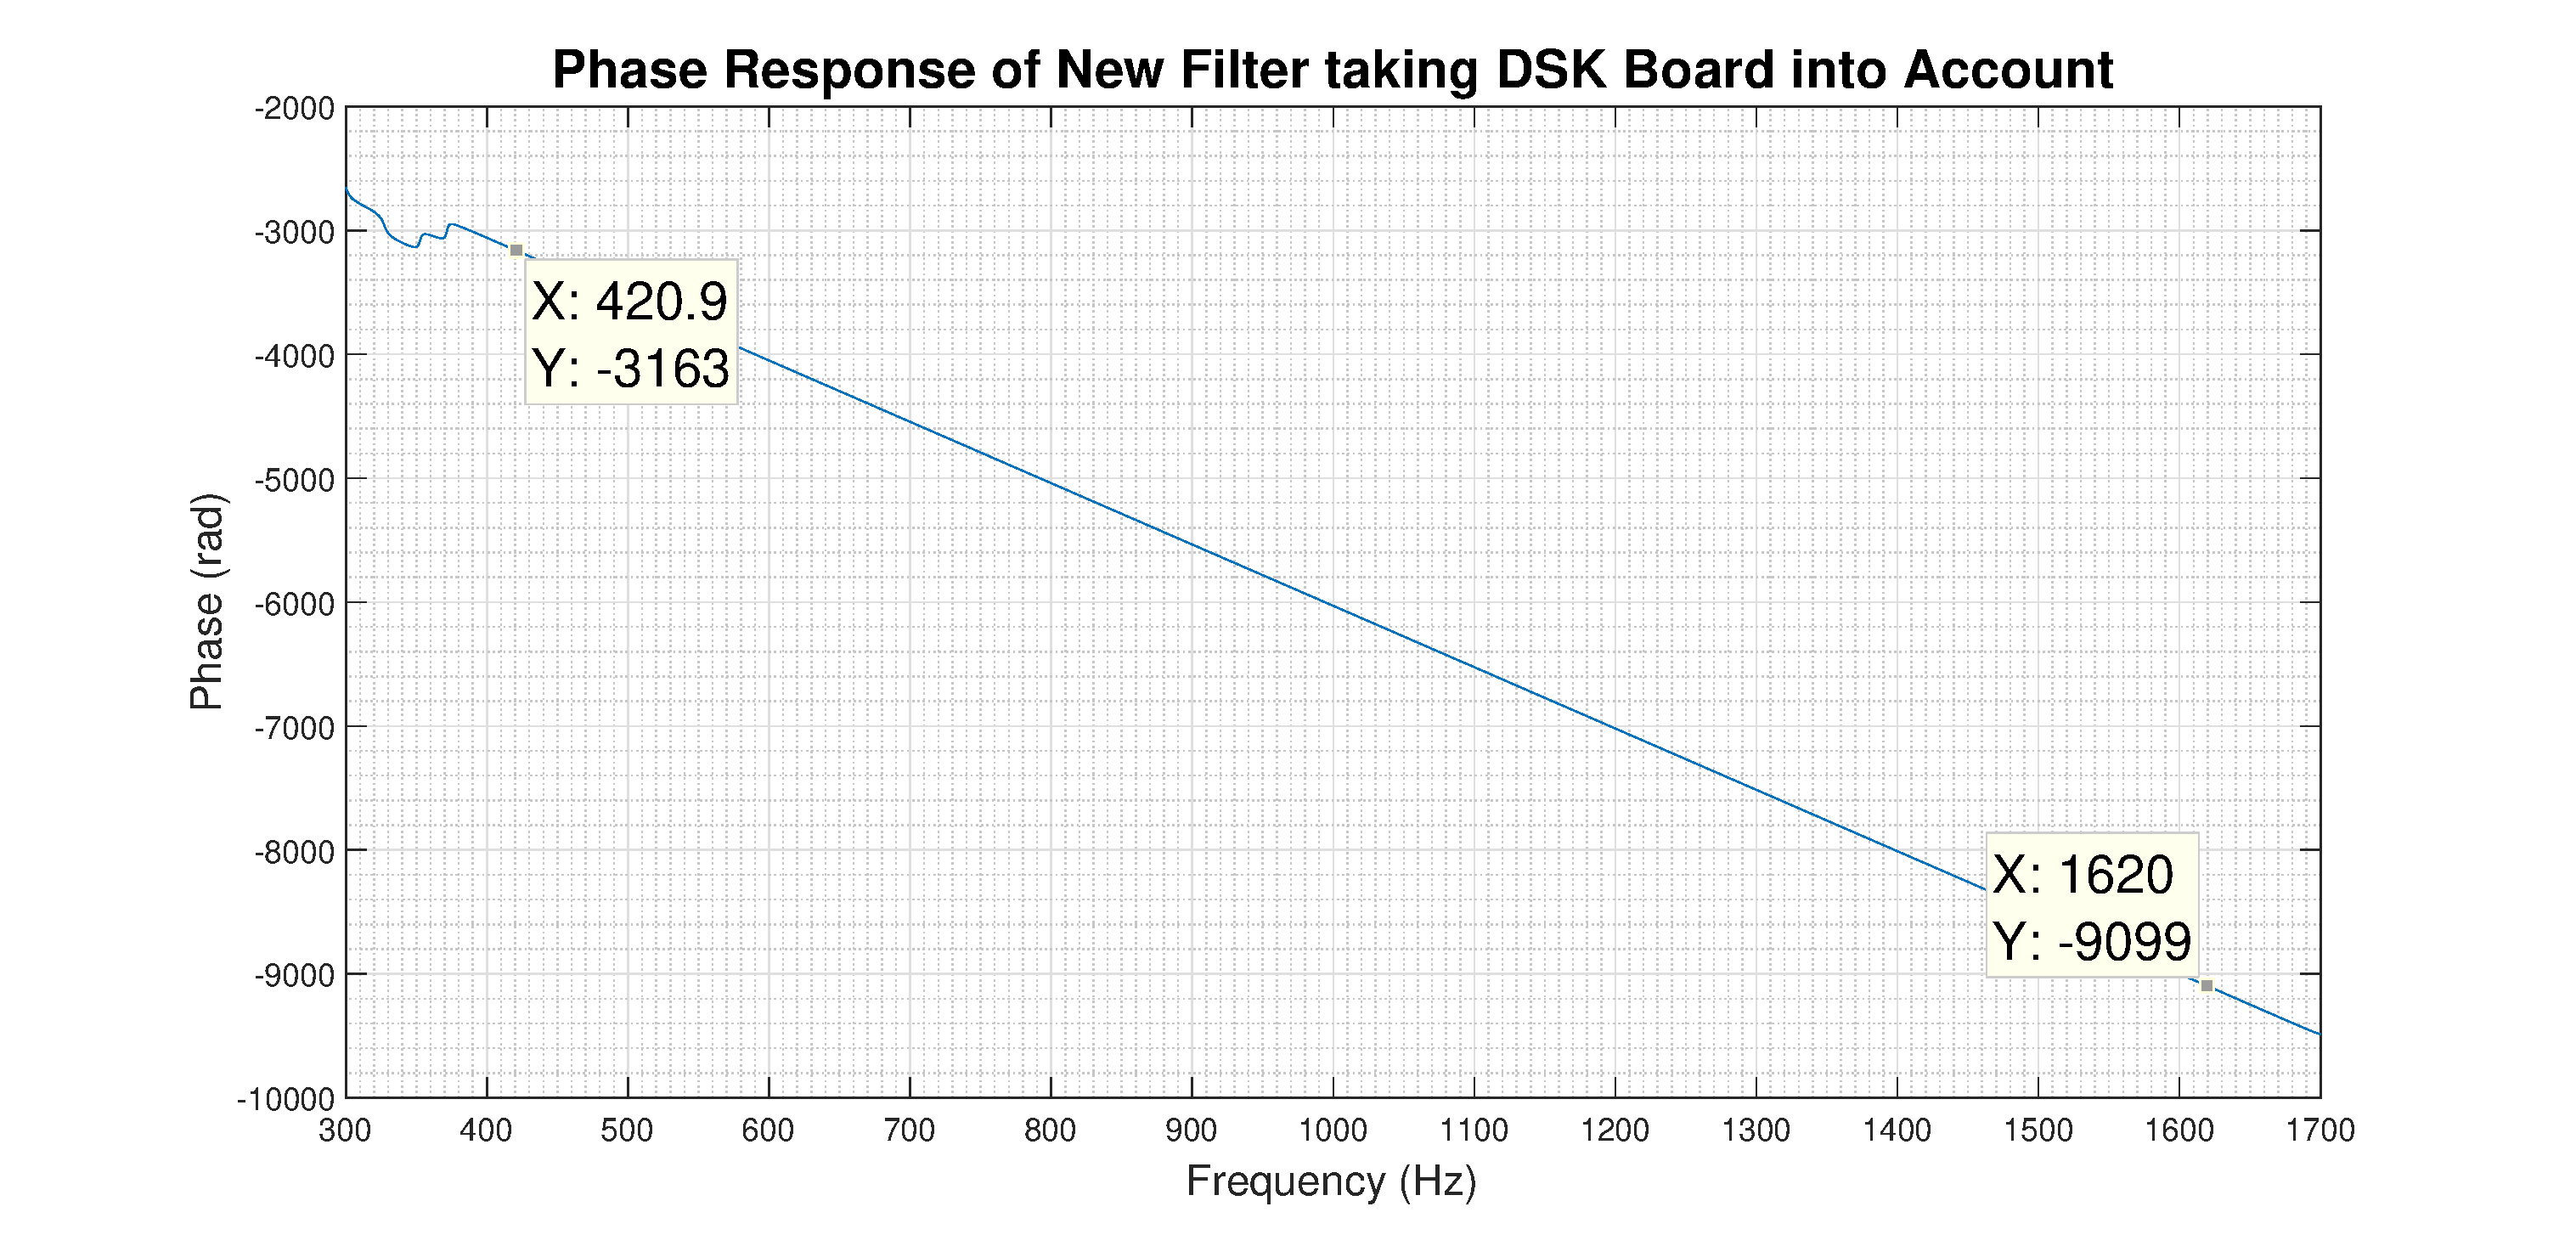
\includegraphics[width=0.80\textwidth]{dsk_phase_new_filter_after_subtracting}
    \caption{Phase response of improved filter}
    \label{fig:new_filter_phase_for_calc}
\end{figure}

Two data cursors are included in the plot. These are the points used to calculate the observed group delay in equation (\ref{eq:group_delay_new_filter_4pm}). 

\begin{equation}\label{eq:group_delay_new_filter_4pm}
    Group\:Delay\:(/s) = -\frac{(\phi_1 - \phi_2)(\tfrac{\pi}{180})}{(\omega_1-\omega_2)(2\pi)} t_s = -\frac{(-3163\cdot10^4 - -9099\cdot10^4)(\tfrac{\pi}{180})}{(420.9-1620)(2\pi)} \frac{1}{8000} = 17.2ms
\end{equation}

The theoretical group delay is calculated in equation (\ref{eq:theo_group_D}).

\begin{equation}\label{eq:theo_group_D}
    Group\:Delay\:(/s) = \frac{M-1}{2} t_s = \frac{221-1}{2} (1/8000) = 13.8ms
\end{equation}

The observed value is approximately equal to the theoretical value. \textbf{The improved filter performs as extremely well both in terms of its magnitude and phase response.}\\

Finally, {\tt circ\_FIR\_symmetric\_pointer} is tested with the new filter. The results obtained are listed in table \ref{tab:final_table}.

\begin{table}[H]
  \centering
    \begin{tabular}{|c|c|c|c|}
    \hline
    \multicolumn{4}{|c|}{New Filter: 221 Coefficients} \\
    \hline
    \multirow{Function} & \multicolumn{3}{c|}{Optimisation} \\
\cline{2-4}          & No Optimisation & Level 0 & Level 2 \\
    \hline
    {\tt circ\_FIR\_symmetric\_ptr} & 7546  & 5497  & \textbf{812} \\
    \hline
    \end{tabular}%
    \caption{Performance measure of {\tt circ\_FIR\_symmetric\_ptr} for new filter}
  \label{tab:final_table}%
\end{table}%

\section{Conclusion}
This report presented the theory behind FIR filters and the discussed generation of filters using the MATLAB functions {\tt firpmord} and {\tt firpm}. A detailed discussion about implementing FIR filters on the $TMS320C6713 \ DSK$ board is presented. \textbf{Compiler optimisations were considered; the function that is expected to be the fastest might not actually be the fastest once compiler optimisations are applied. More details about the type of structures that the compiler recognises and optimises can be found in the Texas Instrument TMS320C6000 Optimisation Compiler User Manual.} Lastly the frequency spectrum of the designed filter was observed. The designed filter did not meet all the specifications and thus a new filter was designed.\\ 

\textbf{The improved filter meet all specifications listed in laboratory 4. The filter was implemented in C and $812$ clock cycles were required for a sample to be read, the convolution sum to be computed and the output to be sent to the AIC23 audio codec. Without including the read or write operation, the filter only required $632$ clock cycles.} 

\newpage
\begin{thebibliography}{99}
\bibitem{ti_comp} 
Instruments, T. (july 2012). TMS320C600 Optimizing Compiler. Retrieved from \url{http://www.ti.com/lit/ug/spru187u/spru187u.pdf}
\end{thebibliography}


\end{document}


